\documentclass[11pt]{amsart}
% Shared preamble of main.tex and supplement.tex. Load after the document class.
\usepackage{amsmath,amssymb,amsthm,mathtools}
\allowdisplaybreaks[1]
\usepackage[margin=1.1in]{geometry}
\setlength{\emergencystretch}{1em}
\usepackage{booktabs,longtable}
\usepackage{xr-hyper}
\usepackage[hidelinks]{hyperref}
\usepackage{refcount}
\usepackage{enumitem}

% ---------------------------------------------------------------- theorem environments
\newtheorem{theorem}{Theorem}[section]
\newtheorem{proposition}[theorem]{Proposition}
\newtheorem{lemma}[theorem]{Lemma}
\newtheorem{corollary}[theorem]{Corollary}
% Lettered results A--G of the introduction.
\newtheorem{maintheorem}{Theorem}
\newtheorem{mainproposition}[maintheorem]{Proposition}
\newtheorem{maincorollary}[maintheorem]{Corollary}
\renewcommand{\themaintheorem}{\Alph{maintheorem}}
\theoremstyle{definition}
\newtheorem{definition}[theorem]{Definition}
\newtheorem{construction}[theorem]{Construction}
\theoremstyle{remark}
\newtheorem{remark}[theorem]{Remark}

% ---------------------------------------------------------------- notation
\newcommand{\R}{\mathbb{R}}
\newcommand{\C}{\mathbb{C}}
\newcommand{\Z}{\mathbb{Z}}
\newcommand{\Q}{\mathbb{Q}}
\newcommand{\N}{\mathbb{N}}
\newcommand{\CP}{\mathbb{CP}}
\newcommand{\eps}{\varepsilon}
\newcommand{\Rcal}{\mathcal{R}}
\newcommand{\Hb}{H_{\mathrm b}}            % base area profile
\newcommand{\Pb}{P_{\mathrm b}}            % unused area
\newcommand{\Bo}{B^{\circ}}                % open capacity ball
\newcommand{\EB}{\mathbb{B}}               % Euclidean ball (radius)
\newcommand{\Pack}{\mathrm{Pack}}          % packing specification
\newcommand{\Hfin}{H_{\mathrm{fin}}}
\newcommand{\defdesc}{\operatorname{the}}   % definite description (never \the, a TeX primitive)
\DeclareMathOperator{\vol}{vol}

% ---------------------------------------------------------------- Lean / blueprint annotations
% Unqualified \lean{...} records references without a claim of complete coverage.
% Optional [full] / [needed] classify coverage in the PDF and generated paper index.
% These are editorial scope annotations, not a machine check of paper/Lean equivalence.
\newcommand{\leancoveragefull}{full statement verified}
\newcommand{\leancoverageneeded}{needed consequence verified}
\newcommand{\lean}[2][]{\if\relax\detokenize{#1}\relax\else
  \ifcsname leancoverage#1\endcsname\else
    \PackageError{paper}{Unknown Lean coverage `#1'}{Use full or needed.}\fi
  \par\nobreak\noindent{\footnotesize\upshape[Lean: \csname leancoverage#1\endcsname.]\par}\nobreak
  \fi\ignorespaces}
% Main-result counterparts agree up to the presentation differences in Section~\ref{sec:ver}.
\newcommand{\leanmark}[1]{\par\nobreak\noindent
  {\footnotesize\upshape\raggedright[Lean: full statement verified; \texttt{#1}]\par}\nobreak}
\newcommand{\uses}[1]{}
\newcommand{\proves}[1]{}

% ---------------------------------------------------------------- cross-document references
% Numbers of the other document carry a prefix: S for the supplement, M for the main text.
% In the main text: \Sref{Lemma}{lem:shd-foo} -> "Lemma S6.3"; \Ssec{sec:shd} -> "\S S6".
% In the supplement: \Mref{Lemma}{lem:eff-gronwall} -> "Lemma M7.1"; the lettered results of
% the main text keep their letters: \Mref{Theorem}{thm:main} -> "Theorem C".
% The second argument is the label WITHOUT the S-/M- prefix.
\makeatletter
\DeclareRobustCommand{\Mprefix}[1]{\edef\@Mref{\getrefnumber{M-#1}}\expandafter\@Mprefix\@Mref\@nil}
\def\@Mprefix#1#2\@nil{\ifnum`#1<`A M\fi}
\makeatother
\newcommand{\Snum}[1]{\href[page=\getpagerefnumber{S-#1}]{supplement.pdf}{S\ref*{S-#1}}}
\newcommand{\Mnum}[1]{\href[page=\getpagerefnumber{M-#1}]{main.pdf}{\Mprefix{#1}\ref*{M-#1}}}
\newcommand{\Sref}[2]{#1~\Snum{#2}}
\newcommand{\Ssec}[1]{\S\Snum{#1}}
\newcommand{\Mref}[2]{#1~\Mnum{#2}}
\newcommand{\Msec}[1]{\S\Mnum{#1}}

\hypersetup{
  pdftitle={Explicit Hamiltonian ball packings in every dimension},
  pdfauthor={Liang Song},
  pdfsubject={Explicit symplectic ball packings and Lean 4 formal verification},
  pdfkeywords={symplectic geometry, Hamiltonian dynamics, ball packing, Lean 4},
  pdflang={en-US}
}
\usepackage{tikz}
\usepackage{array}
\newcolumntype{L}[1]{>{\raggedright\arraybackslash}p{#1}}
\externaldocument[S-]{build/supplement}[supplement.pdf]

\title[Explicit Hamiltonian ball packings]{Explicit Hamiltonian ball packings in every dimension}
\author{Liang Song}
\email{sl12160010@gmail.com}
\thanks{Final version 1.0.0, 29 October 2026. DOI:
\href{https://doi.org/10.5281/zenodo.23756576}{10.5281/zenodo.23756576}.}
\date{}

\begin{document}
\begin{abstract}
Biran's packing stability theorem gives nearly full packings of the four-ball by any $k\ge9$ equal balls. We
construct the motion. For every $k\ge10$ and $\eps\in(0,1)$, one construction defines a smooth compactly
supported Hamiltonian $H_{k,\eps}$ on $\R\times\R^4$ whose time-one map carries the closed unit balls centred at
$(3i-3,0,0,0)$ into the ball of radius $R=(k/(1-\eps/4))^{1/4}$, filling the fraction $1-\eps/4$. This gives a
mathematical solution to the construction problem posed by Epoch AI. The two main ingredients are a linear
comparison function for which the increasing rearrangement of the profile defect is exactly linear, in place of a
contraction fixed point, and a return from the Fermat cubic disc-bundle model to the ball, in which a cube-root symmetry proves
avoidance of the line at infinity. The construction develops the twisted disc-bundle mechanism of a 2026 preprint
of OpenAI and proves four-ball packing stability without $J$-holomorphic curves or Seiberg--Witten theory. In
dimension $2n\ge6$ it realises every packing allowed by the volume and two-ball inequalities, and in dimension
four every packing with $\sum_i c_i^2<C^2$ and $3c_i<C$. We also prove robustness under perturbation with an explicit
margin and give a terminating algorithm whose output is a rational polynomial times a fixed cutoff. The main theorems are
verified in Lean~4.
\end{abstract}
\maketitle

\section{Introduction}\label{sec:intro}

\subsection{The problem}\label{sec:intro-problem}

Points of $\R^{2n}=\C^n$ are $z=(z_1,\dots,z_n)$, $z_j=x_j+iy_j$, the symplectic form is
$\omega_0=\sum_jdx_j\wedge dy_j$, and the Hamiltonian vector field of a function $H(t,z)$ is defined by
$\iota_{X_H}\omega_0=dH$, i.e.\ $X_H=(\partial_{y_1}H,\dots,\partial_{y_n}H,-\partial_{x_1}H,\dots,
-\partial_{x_n}H)$ in the coordinates $(x,y)$. An integral curve of $X_H$ is a differentiable
$\gamma$ with $\gamma'(t)=X_H(t,\gamma(t))$, and $\phi^t_H$ denotes the flow of $X_H$ from time $0$ to
time $t$. We write $B(c)$ for the closed ball of capacity $c$, that is $\{\pi|z|^2\le c\}$, $\Bo(c)$ for its interior,
and $B(s,c)=s+B(c)$ for $s\in\R^{2n}$.

A \emph{symplectic packing} of a ball by finitely many balls is a family of symplectic embeddings of the balls into
the ball with pairwise disjoint images. Since $\vol B(c)=c^n/n!$, balls of capacities $c_1,\dots,c_k$ can be packed
into $\Bo(C)$ only if $\sum_ic_i^n<C^n$, and Gromov's two-ball theorem \cite{Gromov1985} gives the second obstruction
$c_i+c_j<C$ for $i\ne j$. In dimension four there are further obstructions: five balls of capacity $\frac{11}{25}$
satisfy both inequalities, but the fifth ECH capacity of their union is at least $\frac{11}5$, and that of $\Bo(1)$ is
$2$ \cite{Hutchings2011}.

In dimension four the existence question is settled. Biran \cite{Biran1997} showed that for every $k\ge9$ and every $c$
with $kc^2<C^2$, $k$ balls of capacity $c$ embed in $\Bo(C)$, and the work of McDuff--Polterovich, McDuff, Li--Liu and
Li--Li \cite{McDuffPolterovich1994,McDuff1998,LiLiu2001,LiLi2002} reduces every four-dimensional ball packing problem to
a list of inequalities indexed by exceptional classes. These proofs use $J$-holomorphic curves and, through Taubes'
theorem and inflation on blow-ups of $\CP^2$, Seiberg--Witten theory. They show that embeddings exist; they do not
produce a Hamiltonian that moves given balls into the target. Explicit full packings for square $k$, and several other constructive methods, are discussed in
\S\ref{sec:intro-prior}. Here the goal is one Hamiltonian construction for every $k\ge10$ and every positive error.

Epoch AI \cite{Epoch} asked for such a motion: for every integer $k\ge10$ and every $\eps\in(0,1)$, an algorithm
that, on input $(k,\eps)$, outputs an explicit smooth time-dependent Hamiltonian $H(t,z)$ on $\R^4$ whose time-one map sends the closed unit
balls centred at $(3i-3,0,0,0)$, $1\le i\le k$, into a closed ball $B^4(R)$ of Euclidean radius $R$ centred at the
origin, with $k/R^4>1-\eps$. Since the flow preserves volume, $k/R^4$ is the fraction of $B^4(R)$ filled by the
images. The construction below supplies one Hamiltonian for each $(k,\eps)$, defined by the same formulas
for all of them; Theorem~\ref{thm:eff-algorithm} supplies a uniform algorithm with finite output.
Remark~\ref{rem:eff-epoch-interface} relates these results to Epoch's program submission format.

\subsection{The four-dimensional theorem}\label{sec:intro-contribution}

For admissible data (Definition~\ref{def:intro-admissible}) we define in \S\ref{sec:ham} one Hamiltonian
$H[n,k,C,c,s]$ (Definition~\ref{def:ham-H-final}), by a construction that is the same for all data. The first theorem is its
four-dimensional instance for the data of the Epoch question.

\begin{maintheorem}[Equal balls in the four-ball]\label{thm:intro-4d}
\uses{def:ham-H-final, def:intro-spec, prop:cmp-linear, thm:main}
Let $k\ge10$ be an integer and $\eps\in(0,1)$. Put
\[
 R=\left(\frac{k}{1-\eps/4}\right)^{1/4},\qquad C=\pi R^2,\qquad s_i=(3i-3,0,0,0)\in\R^4\quad(1\le i\le k),
\]
and $H_{k,\eps}=H[2,k,C,(\pi,\dots,\pi),(s_1,\dots,s_k)]$. Then $H_{k,\eps}$ is $C^\infty$ on $\R\times\R^4$, vanishes
for $t\notin(0,1)$ and outside $\R\times\mathcal S$ for an explicit compact set $\mathcal S$, and satisfies
$\Pack(2,k,C,(\pi,\dots,\pi),s)$ (Definition~\ref{def:intro-spec}): its flow is global, and its time-one map sends each
closed unit ball $B(s_i,\pi)$ into $\Bo(\pi R^2)$, the open Euclidean ball of radius $R$ about the origin, with pairwise
disjoint images. Moreover $k/R^4=1-\eps/4>1-\eps$.
\leanmark{four\_dim\_theorem, main\_time\_support, main\_support\_radius, flow\_images\_disjoint}
\end{maintheorem}

\begin{proof}
The centres are at distance at least $3$, so the closed unit balls are disjoint. Since $R^4=k/(1-\eps/4)>k\ge10$, we
have $k\pi^2<\pi^2R^4=C^2$ and $3\pi<\pi R^2=C$, so $(2,k,C,(\pi,\dots,\pi))$ is admissible and
Theorem~\ref{thm:main}(i) below applies. For these data the normalised capacity $\rho=\pi/C=R^{-2}$ satisfies
$\rho\sqrt k=\sqrt{1-\eps/4}>\sqrt3/2>\frac34$, which selects the linear comparison datum of
Proposition~\ref{prop:cmp-linear} in \Sref{Construction}{cons:ham-branch}.
\end{proof}

The theorem leaves an explicit margin. The images lie in the closed ball of radius $R$, while the density requirement
$k/R'^4>1-\eps$ is already met by $R'=(k/(1-\eps/2))^{1/4}>R$. The following estimate converts this margin, a closed
formula in $(k,\eps)$, into a tolerance on the vector field.

\begin{mainproposition}[Robustness]\label{thm:intro-stability}
Let $k\ge10$, $\eps\in(0,1)$, and let $R<R'$ be as above. Let $\widehat H$ be a smooth function on $\R\times\R^4$
vanishing outside $\R\times K$ for a compact set $K$. Suppose that, for $t\in[0,1]$, the field $X_{\widehat H}(t,\cdot)$
is $L$-Lipschitz for some $L\ge0$ and $|X_{\widehat H}-X_{H_{k,\eps}}|\le\eta$ on $\R^4$, where $\eta e^L\le R'-R$. Then the time-one map
of $\widehat H$ sends each closed unit ball $B(s_i,\pi)$ into the closed ball of radius $R'$ about the origin, and
$k/R'^4=1-\eps/2>1-\eps$.
\leanmark{four\_dim\_stability}
\end{mainproposition}

\begin{proof}
Let $\gamma$ and $\hat\gamma$ be integral curves of $X_{H_{k,\eps}}$ and $X_{\widehat H}$ starting at the same point of
$B(s_i,\pi)$. Then $|\hat\gamma(1)-\gamma(1)|\le\eta(e^L-1)/L\le\eta e^L$ by Gr\"onwall's inequality
(Lemma~\ref{lem:eff-gronwall}, with the Lipschitz bound on $X_{\widehat H}$), and $|\gamma(1)|\le R$ by
Theorem~\ref{thm:intro-4d}. For $L=0$ the Gr\"onwall bound is $\eta$.
\end{proof}

Thus every smooth compactly supported approximation with vector-field error at most $(R'-R)e^{-L}$ still meets the
Epoch requirement, with images in the ball of radius $R'$; the geometric margin $R'-R$ depends only on $(k,\eps)$. Theorem~\ref{thm:eff-algorithm} gives one
algorithm which, on input $k$ and a name of $\eps$, halts with $B\in\N$ and $P\in\Q[t,z]$ such that $\beta_B\cdot P$, a
rational polynomial times a fixed smooth cutoff, satisfies the same packing specification. Each output is certified by
a finite rational test, and the construction shows that the search terminates.

The packings of Theorem~\ref{thm:intro-4d} exist by Biran's theorem. The proof here works with explicit maps, forms and
flows only and uses none of the existence results quoted above. Through Corollary~\ref{thm:main-equal} it gives a proof
of Biran's packing stability for $B^4$ without $J$-holomorphic curves or Seiberg--Witten theory, which the earlier
proofs \cite{Biran1997,Biran1999,BuseHind2013,BuseHindOpshtein2016} use, directly or through the results they cite.

\subsection{The mechanism}\label{sec:intro-mechanism}

The construction follows a mechanism due to the OpenAI preprint \cite{OpenAI2026}. We describe it in dimension four, where the picture is
classical. Give $\CP^2$ the Fubini--Study form for which a line has area $1$, so that $\vol\CP^2=\frac12$ and the
complement of a line is $\Bo(1)$. Let $E\subset\CP^2$ be a smooth cubic, of area $3$. Biran \cite{Biran2001} showed
that the complement of an isotropic skeleton in $\CP^2$ is symplectomorphic to a disc bundle over $E$: the normal
bundle, of degree $E\cdot E=9$, with fibre discs of capacity $\frac13$. With fibre moment $p=\pi|w|^2$, the base area
of the circle bundle at level $p$ is
\[
 A(p)=3-9p=3(1-3p)\qquad(0\le p<\tfrac13),\qquad \int_0^{1/3}A(p)\,dp=\frac12=\vol\CP^2 .
\]
The cubic is the first smooth plane curve with the topology needed by this handle construction. Its closed base
must carry a closed one-form $\beta$ with nonzero period around the handle. A line or conic has genus zero, so
$H^1(S^2;\R)=0$ rules out such a form; a cubic has genus one. Thus the fibre bound $\frac13$, and hence $3c_i<C$,
reflects the choice of the smallest-degree smooth plane curve supporting this mechanism.

A ball $B(a)\subset\C\times\C$, sliced by the moment $p$ of its second coordinate, is a family of discs of capacity
$a-p$ for $p\le a$; its slice profile is $(a-p)_+$, and $\int_0^\infty(a-p)_+\,dp=a^2/2=\vol B(a)$. Placing balls
fibrewise in the bundle requires $a<\frac13$: this is the source of the condition $3c_i<C$. If
$\sum_i(a_i-p)_+\le A(p)$ for every $p$, the base discs can be placed side by side over $E$. For nine balls of
capacity $\frac13$ this holds with equality. For $k\ge10$ balls of capacity close to $1/\sqrt k$ the integrated
inequality $\sum_ia_i^2/2<\frac12$ holds, but at $p=0$ one needs $\sum_ia_i\le3$, which fails: the difference
$A(p)-\sum_i(a_i-p)_+$ has positive integral and is negative near $p=0$ (Figure~\ref{fig:intro-profile}).

\begin{figure}[ht]
\centering
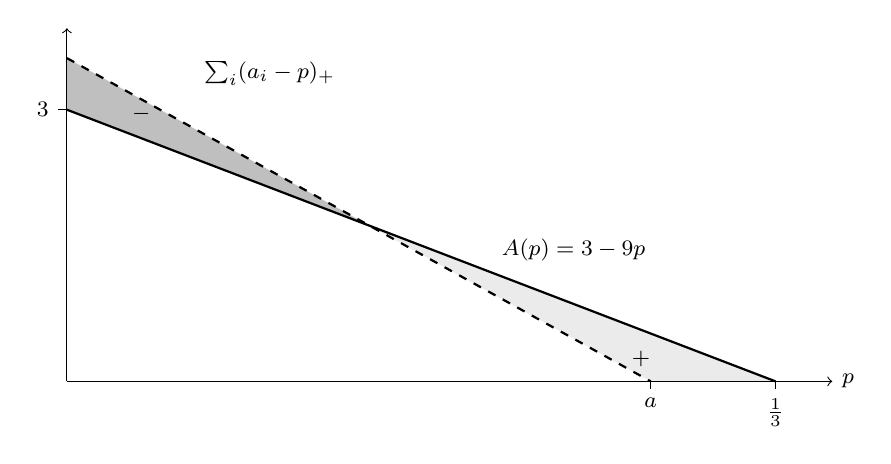
\begin{tikzpicture}[x=27cm,y=1.15cm,font=\footnotesize]
 % deficit and surplus regions for k=13, a=0.99/sqrt(13)=0.2746, h=0.33
 \fill[black!25] (0,3) -- (0,3.570) -- (0.1424,1.718) -- cycle;
 \fill[black!8] (0.1424,1.718) -- (0.2746,0) -- (0.33,0) -- (0.33,0.03) -- cycle;
 \draw[->] (0,0) -- (0.36,0) node[right] {$p$};
 \draw[->] (0,0) -- (0,3.9);
 \draw[thick] (0,3) -- (0.3333,0);
 \draw[thick,dashed] (0,3.570) -- (0.2746,0);
 \draw (0.3333,0) -- (0.3333,-0.08) node[below] {$\tfrac13$};
 \draw (0.2746,0) -- (0.2746,-0.08) node[below] {$a$};
 \draw (0,3) -- (-0.004,3) node[left] {$3$};
 \node[right] at (0.06,3.4) {$\sum_i(a_i-p)_+$};
 \node[right] at (0.2,1.45) {$A(p)=3-9p$};
 \node at (0.035,2.95) {$-$};
 \node at (0.27,0.25) {$+$};
\end{tikzpicture}
\caption{The area profile $A$ of the cubic model (solid) and the slice profile of $13$ balls of capacity
$a=0.99/\sqrt{13}$ (dashed). The deficit (dark) is smaller than the surplus (light), since
$\int_0^h(A-\sum_i(a_i-p)_+)\,dp=\frac12(1-13a^2-(1-3h)^2)>0$ for $h=0.33$, but stacking needs $A\ge\sum_i(a_i-p)_+$
pointwise. The twist moves area from the surplus to the deficit.}
\label{fig:intro-profile}
\end{figure}

The construction of \cite{OpenAI2026} pays the deficit with the surplus by twisting the bundle. Across an
annulus in the base, the fibre over one boundary circle is identified with the fibre over the other by an
area-preserving map $q$ of the fibre disc instead of the identity. Paired with a function $K$ of the moment, the
twist changes the base area available above a fibre point $w$ from $A(p(w))$ to
$A(p(w))+K(p(q^{-1}w))-K(p(w))$ (equation~\eqref{eq:mech-available}). Since $q$ preserves the fibre area, this
redistributes area between moment levels without changing the total. The balls fit if, for some $\gamma>0$ and
$P=A-\sum_i(a_i-p)_+$,
\[
 (K-P)\bigl(p(q(w))\bigr)\le K\bigl(p(w)\bigr)-\gamma\qquad\text{for every fibre point }w.
\]
This forces $\int P>0$. Conversely, for concave $P$ with positive mean that is positive outside a core,
\cite{OpenAI2026} obtains $K$ as the fixed point of a contraction built from increasing rearrangements, realises the
rearrangements by isotopies, and turns the inequality into embeddings by Moser's method and a transfer to the target.
For $k\ge10$ equal balls with $\frac34<\rho\sqrt k<1$ a linear $K$ suffices: $K-P$ is, up
to a constant, a tent whose increasing rearrangement is linear, and the inequality becomes an identity up to the error
of one planar map (Proposition~\ref{prop:cmp-linear}).

\subsection{The main steps}\label{sec:intro-steps}

The four-dimensional contribution consists of four constructions, listed in Table~\ref{tab:intro-steps}: the linear
comparison identity, which removes the fixed-point step for the Epoch family; an explicit planar rearrangement; a
symmetry-controlled return from the Fermat cubic model, written in explicit cover coordinates, to the affine ball;
and one global motion from the prescribed source balls. We first give the construction chain for
Theorem~\ref{thm:intro-4d}.

\emph{The construction chain.} After the dilation by $1/\sqrt C$ the target is $\Bo(1)$ and each ball has capacity $\rho$.
Put $\eta_\star=1-\sqrt{1-\eps/4}$, $t_0=1-\eta_\star/2$, $a=t_0/\sqrt k$, $h=t_0/3$ and $g=3\eta_\star/2$. Then $H_{k,\eps}$ is
obtained in five steps, each determined by the data and by the previous steps.
\begin{enumerate}[label=(\arabic*)]
\item \emph{Model.} The cubic disc-bundle model associated with Biran's decomposition, written on the cover $\R^2\times\C$ of the Fermat torus with the
 explicit form $\Omega_0$ of \S\ref{sec:mdl-cub}, cut at fibre moment $p\le h$.
\item \emph{Comparison.} The linear function $K(p)=(3\sqrt k-9)p$ and the fibre isotopy $(q_t)$ of
 \Sref{Theorem}{thm:pll-inner}, generated by an explicit planar Hamiltonian; its endpoint carries the centred disc of
 area $I$ into the sublevel set $\{\Lambda\circ p\le I+4e_q\}$ of the tent $\Lambda$ of \S\ref{sec:cmp-linear}, with $e_q$ as there. The
 comparison gap is $\frac{31}{32}g$ (Proposition~\ref{prop:cmp-linear}).
\item \emph{Handle.} Over an annulus $\mathcal A$ in the base, the bundle chart $\chi_{\mathcal A}$ and the twist
 $\mathcal D$, which applies $q_{f(s)}$ to the fibre over the handle coordinate $s$ for a fixed clock $f$; the Moser map
 $\Phi$, the time-one map of three explicit fields; the layer maps $E_i$, given by an explicit strip map and unique
 roots (\S\ref{sec:hdl}, Remark~\ref{rem:hdl-four}).
\item \emph{Return.} The map $\mathcal T=b_{\rm ball}\circ\psi_1^{-1}\circ\mathrm{pr}\circ\tau_1\circ\iota\circ\mathsf N$
 from the model into $\Bo(1)$: it carries the model into $\CP^2$ minus the line $\{Z_0=0\}$, which the ball chart
 $b_{\rm ball}$ identifies with $\Bo(1)$; $\tau_1$ and $\psi_1$ are time-one maps of explicit ordinary differential
 equations (\Ssec{sec:rtc}). The embeddings are
 \[
  f_i(u)=\sqrt C\,\bigl(\mathcal T\circ\Phi^{-1}\circ\chi_{\mathcal A}\circ\mathcal D^{-1}\circ E_i\bigr)(u/\sqrt C)
 \]
 (\Sref{Remark}{rem:cub-lean}).
\item \emph{Motion.} One isotopy $F_{i,t}$ from the translations $u\mapsto s_i+u$ to the $f_i$, with disjoint images at all
 times (Proposition~\ref{prop:ham-isotopy}), and $H_{k,\eps}$, the pushforward along it of a radial primitive computed in
 the source balls (Definition~\ref{def:ham-H}).
\end{enumerate}
The parameters $t_0$, $a$, $h$, $g$, the slope of $K$ and the height $d_n=\frac13-\frac{\eta_\star}{12}$ used by the return are
closed-form expressions in $\sqrt k$ and $\eps$ (\Sref{Remark}{rem:rtc-equal}); the maps are formulas, integrals,
time-one maps of explicit vector fields, inverses of explicit injective maps and extrema over explicit compact sets.

Table~\ref{tab:intro-steps} lists the four constructions with the statements that resolve them. The handle step (3)
follows \cite{OpenAI2026} with explicit fields once the comparison datum is given.

\begin{table}[ht]
\centering\footnotesize
\renewcommand{\arraystretch}{1.15}
\begin{tabular}{@{}L{0.15\textwidth}L{0.53\textwidth}L{0.26\textwidth}@{}}
\toprule
Step & What is needed, and the difficulty & Core statement\\
\midrule
comparison & a finite datum $(K,q)$ with a quantitative gap in place of the fixed point of a contraction; for equal balls
 in dimension four, a linear $K$ for which the comparison is an identity up to the planar error &
 Prop.~\ref{prop:cmp-linear}; Thm.~\ref{thm:cmp-main}\\
planar rearrangement & an area-preserving disc map carrying round discs into prescribed sublevel sets: a convex potential whose
 sublevel areas follow the increasing rearrangement, made quadratic near its minimum; a Morse chart with rotation and area normalisation; a Hamiltonian
 path on the whole disc, the identity near the boundary, ending at this map on a core &
 Thm.~\ref{thm:cmp-realisation}; \Sref{Thms.}{thm:pln-inner}, \Snum{thm:pln-isotopy}, \Snum{thm:pll-inner}\\
return to the ball & explicit coordinates on the cover of the Fermat cubic and explicit transport and return fields
 carrying the model form to the Fubini--Study form; proof that the images avoid the line at infinity $\{Z_0=0\}$, and
 are injective modulo deck maps, with a compact margin inside $\Bo(1)$ &
 Thm.~\ref{thm:mdl-cub}; \Sref{Thm.}{thm:rtc-transfer}, \Sref{Prop.}{prop:rtc-avoid}\\
from the given balls & one isotopy from the prescribed balls to the model embeddings keeping the closed balls disjoint
 at all times (a route ordered by ranks, a path in $\operatorname{Sp}(2n)$, a shape stage, a common dilation), and
 a global Hamiltonian generating it on the balls &
 Props.~\ref{prop:ham-isotopy}, \ref{prop:ham-end}; \Sref{Prop.}{prop:iso-common}\\
\bottomrule
\end{tabular}
\caption{The main steps of the construction and the statements that resolve them.}
\label{tab:intro-steps}
\end{table}

The linear comparison identity and the symmetry argument for the return are the two simplifications particular
to the four-dimensional construction. Together with the planar rearrangement and the common isotopy, they turn
the disc-bundle mechanism into an explicit motion of the given balls. The parameters are fixed uniformly in the
data, and the margins pass quantitatively from step to step: the comparison gap
$\frac{31}{32}g$ pays for the planar error and for the excess of the handle caps over the ball profiles, the return
leaves a compact margin inside $\Bo(1)$, and the isotopy uses explicit radii between the closed balls and the domains of
the embeddings. Each map is defined on the whole domain on which the next one uses it: the planar isotopy on the
whole disc, the Moser flows on the whole model, the Hamiltonian on $\R\times\R^{2n}$.

\subsection{All dimensions and unequal balls}\label{sec:intro-results}

In dimension $2n\ge6$ the volume and two-ball inequalities are the only obstructions to packing a ball by balls: this
is Conjecture~A of Siegel and Yao \cite{SiegelYao2025}, proved in a 2026 preprint of OpenAI \cite{OpenAI2026}.
The construction of Theorem~\ref{thm:intro-4d} extends to these problems and to unequal balls in
dimension four.

\begin{definition}[Packing specification]\label{def:intro-spec}
\lean{SymplecticPacking.Problem.PackingSpec}
Let $n\ge1$, $k\ge0$, $C>0$, $c=(c_1,\dots,c_k)\in(0,\infty)^k$ and $s=(s_1,\dots,s_k)\in(\R^{2n})^k$. A
function $H\colon\R\times\R^{2n}\to\R$ satisfies $\Pack(n,k,C,c,s)$ if
\begin{enumerate}[label=(\alph*)]
\item $H$ is $C^\infty$, and there is a compact set $\mathcal S\subset\R^{2n}$ with $H(t,z)=0$ for all
 $t\in\R$ and all $z\notin\mathcal S$;
\item for every $i$ and every $z\in B(s_i,c_i)$ there is an integral curve $\gamma\colon\R\to\R^{2n}$ of
 $X_H$ with $\gamma(0)=z$, and every integral curve $\gamma\colon[0,1]\to\R^{2n}$ of $X_H$ with
 $\gamma(0)=z$ satisfies $\gamma(1)\in\Bo(C)$.
\end{enumerate}
\leanmark{Problem.PackingSpec}
\end{definition}

For $H$ satisfying (a) the flow $\phi^t_H$ is global and consists of symplectic diffeomorphisms, and
(b) says $\phi^1_H(B(s_i,c_i))\subset\Bo(C)$ for every $i$.

\begin{definition}[Admissible data]\label{def:intro-admissible}
\lean{SymplecticPacking.Problem.Admissible}
Let $n\ge2$, $k\ge1$, $C>0$ and $c\in(0,\infty)^k$. The data $(n,k,C,c)$ are \emph{admissible} if
\begin{align*}
 n\ge3:&\qquad \textstyle\sum_ic_i^n<C^n\quad\text{and}\quad c_i+c_j<C\ \text{ for all } i\ne j;\\
 n=2:&\qquad \textstyle\sum_ic_i^2<C^2\quad\text{and}\quad 3c_i<C\ \text{ for all } i.
\end{align*}
\leanmark{Problem.Admissible}
\end{definition}

For $n\ge3$ admissibility is exactly the pair of necessary conditions above. For $n=2$ the condition
$3c_i<C$ is stronger than the two-ball inequality; admissible data include $k\ge9$ equal balls with
$kc^2<C^2$ and the unequal capacity vectors of Corollary~\ref{thm:main-cone4}. This is a sufficient small-capacity
range, for any $k\ge1$, rather than the full four-dimensional packing criterion.

\begin{maintheorem}\label{thm:main}
\uses{def:intro-spec, def:intro-admissible, def:intro-levels, def:ham-H-final, thm:eff-algorithm}
Let $n\ge2$, $k\ge1$, $C>0$, $c_1,\dots,c_k>0$ and $s_1,\dots,s_k\in\R^{2n}$ be such that the closed balls
$B(s_i,c_i)$ are pairwise disjoint and $(n,k,C,c)$ is admissible. Then:
\begin{enumerate}[label=(\roman*)]
\item the function $H=H[n,k,C,c,s]$ of Definition~\ref{def:ham-H-final} is $C^\infty$ on $\R\times\R^{2n}$,
 vanishes outside $\R\times\mathcal S$ for an explicit compact set $\mathcal S$ and for $t\notin(0,1)$, and
 satisfies $\Pack(n,k,C,c,s)$; in particular $\phi^1_H$ maps each $B(s_i,c_i)$ into $\Bo(C)$, and the
 images are pairwise disjoint;
 \leanmark{main\_theorem, main\_time\_support, main\_support\_radius, flow\_images\_disjoint}
\item \textup{(L1)} the definition of $H[n,k,C,c,s]$ is the same for all such data and uses only the
 operations of level~L1 in Definition~\ref{def:intro-levels};
\item \textup{(L2, L3)} there is one oracle algorithm which, given $n$, $k$ and names of the real inputs
 $C,c_1,\dots,c_k,s_1,\dots,s_k$ (a rational number is named by its constant sequence), halts on all such data and
 outputs an integer $B$ and a polynomial $P\in\Q[t,z]$ such that $\Hfin=\beta_B\cdot P$ satisfies
 $\Pack(n,k,C,c,s)$. The output may depend on the names; for computable inputs, given by computable names, it is an
 ordinary algorithm.
 \leanmark{original\_name\_algorithm}
\end{enumerate}
\end{maintheorem}

Parts (i) and (ii) are proved in \S\ref{sec:ham-proof-main}, part (iii) is
Theorem~\ref{thm:eff-algorithm}. Part~(ii) is a statement about the definition: Table~\ref{tab:ham-explicit}
lists, for each ingredient of $H[n,k,C,c,s]$, the operation of Definition~\ref{def:intro-levels} that produces
it; none of them is a search over Hamiltonians, maps or packings.

For $2n\ge6$ the fibre of the model is $\C^{n-1}$ and the base a compact piece of an affine curve, the diagonal
curve $y_j^2=t^2-j$ for capacities below $\frac12$; the two-ball inequality allows at most one ball of capacity at
least $\frac12$, which is reserved while the others are packed in a model of its complement
(Table~\ref{tab:mech-models}). The comparison datum is the finite rational iterate of Theorem~\ref{thm:cmp-main}.
In dimension four, inputs other than those of Theorem~\ref{thm:intro-4d}, including $k=9$ and unequal capacities, use
the scalar comparator of \Ssec{sec:scalar-cmp}; the handle construction for $n=2$ is summarised in Remark~\ref{rem:hdl-four} and carried out in
\Ssec{sec:shd-four}.

The packings of Theorem~\ref{thm:main} also exist by known results. For $n\ge3$ this is \cite{OpenAI2026}. For $n=2$, by \cite{McDuffPolterovich1994,McDuff1998,LiLiu2001,LiLi2002}, closed balls
of capacities $c_i$ embed in $\Bo(C)$ if $\sum_ic_i^2<C^2$ and $\sum_im_ic_i<dC$ for every exceptional class
$(d;m_1,\dots,m_k)$ with $d\ge1$; such a class has $m_i\ge0$ and $\sum_im_i=3d-1$, so $3c_i<C$ gives
$\sum_im_ic_i<(3d-1)C/3<dC$. The threshold $k\ge9$ of Corollary~\ref{thm:main-equal} is Biran's \cite{Biran1997}.

\begin{maincorollary}[The Siegel--Yao criterion by explicit flows]\label{thm:main-sy}
Let $n\ge3$, $k\ge1$, $C>0$ and $c_i>0$, and let $B(s_i,c_i)\subset\R^{2n}$, $1\le i\le k$, be pairwise disjoint closed balls.
There is a symplectic embedding of a neighbourhood of $\bigsqcup_iB(s_i,c_i)$ into $\Bo(C)$ if and only if
$\sum_ic_i^n<C^n$ and $c_i+c_j<C$ for all $i\ne j$. In that case $\phi^1_H$ with $H=H[n,k,C,c,s]$ is such
an embedding.
\leanmark{neighbourhood\_criterion, flow\_neighbourhood\_embedding}
\end{maincorollary}

Necessity follows from volume and from Gromov's two-ball theorem, whose proof uses $J$-holomorphic lines.
Sufficiency is the main theorem of \cite{OpenAI2026}; Corollary~\ref{thm:main-sy} reproves it by explicit flows,
without $J$-holomorphic curves, and realises every such packing by the time-one map of an explicit Hamiltonian.

\begin{maincorollary}[Equal balls]\label{thm:main-equal}
Let $n\ge2$, $\eps\in(0,1)$, and $k\ge2^n$ if $n\ge3$, $k\ge9$ if $n=2$. Let $c>0$, let $s_1,\dots,s_k$ be
centres with $B(s_i,c)$ pairwise disjoint, and let $C>0$ with $kc^n<C^n<kc^n/(1-\eps)$. Then
$H[n,k,C,(c,\dots,c),s]$ satisfies $\Pack(n,k,C,(c,\dots,c),s)$, and $kc^n/C^n>1-\eps$.
\leanmark{equal\_balls}
\end{maincorollary}

Since $\phi^1_H$ preserves volume and the images are disjoint, they fill the fraction $kc^n/C^n$ of the volume of
$B(C)$. For $n\ge3$ and $k\ge2$ the bound $k\ge2^n$ is forced by the two-ball inequality, since $2\le k<2^n$ equal
balls fill at most $k/2^n$ of a ball. For $n=2$ the bound $k\ge9$ comes from the condition $3c<C$; for $k\le8$ full packings
do not exist except for $k=1,4$ \cite{McDuffPolterovich1994}.

\begin{maincorollary}[The Epoch data]\label{thm:main-epoch}
Let $k\ge9$ be an integer, $\eps\in(0,1)$, $s_i=(3i-3,0,0,0)\in\R^4$, $R=(k/(1-\eps/2))^{1/4}$ and $C=\pi R^2$. Then
$H=H[2,k,C,(\pi,\dots,\pi),s]$ satisfies $\Pack(2,k,C,(\pi,\dots,\pi),s)$: its time-one map sends each closed unit ball
$B(s_i,\pi)$ into $\Bo(\pi R^2)$, the open Euclidean ball of radius $R$ about the origin, and $k/R^4=1-\eps/2>1-\eps$.
\leanmark{epoch\_packing, epoch\_theorem\_ten}
\end{maincorollary}

Theorem~\ref{thm:intro-4d} is the case $k\ge10$ of Corollary~\ref{thm:main-epoch} at $\eps/2$. At density
$1-\eps/2$ the linear comparison datum applies for $k\ge10$ and $\eps<\frac78$; the remaining cases use the scalar
comparator. The corollary is the form used by the Epoch machine of Theorem~\ref{thm:eff-algorithm}: on input $k$ and a name of $\eps$ it outputs $(B,P)$
such that $\beta_B\cdot P$ satisfies the same specification.

\begin{maincorollary}[A cone of unequal balls in dimension four]\label{thm:main-cone4}
Let $k\ge1$ and $c_1,\dots,c_k>0$ with $\max_ic_i\le\frac13\big(\sum_ic_i^2\big)^{1/2}$, let $\eps\in(0,1)$ and
$C_\eps=\big(\sum_ic_i^2/(1-\eps/2)\big)^{1/2}$. For all centres $s_i$ with $B(s_i,c_i)$ pairwise disjoint,
$H[2,k,C_\eps,c,s]$ satisfies $\Pack(2,k,C_\eps,c,s)$, and $\sum_ic_i^2/C_\eps^2=1-\eps/2$; the images fill the fraction
$1-\eps/2$ of the volume of $B(C_\eps)$.
\leanmark{unequal\_cone}
\end{maincorollary}

\begin{proof}[Proofs of Corollaries~\ref{thm:main-sy}--\ref{thm:main-cone4}]
The sufficiency statements follow from Theorem~\ref{thm:main} after checking admissibility; the necessity in
Corollary~\ref{thm:main-sy} uses the classical obstructions. See \S\ref{sec:ham-proof-main}.
\end{proof}

\subsection{Explicitness and the finite output}\label{sec:intro-explicitness}

The Hamiltonians of Theorems~\ref{thm:intro-4d} and~\ref{thm:main} are explicit in the following graded sense.

\begin{definition}[Levels of explicitness]\label{def:intro-levels}
\begin{enumerate}[label=(L\arabic*)]
\item An \emph{explicit definitional construction} is a definition built from rational constants and the
 input by arithmetic and elementary functions, integrals over compact domains, limits of series with an
 explicit rate of convergence, maxima and minima of continuous functions over explicit compact sets,
 unique solutions of explicit ordinary differential equations, inverses of explicit injective maps,
 unique roots of explicit equations, case distinctions on propositions about the input and about the arguments of
 the function being defined, and least
 elements of searches over a fixed enumeration of finitely described objects (integers, rationals, and
 tuples of these and of rational polynomials) whose validity is decided by finitely many explicit
 inequalities; definite descriptions are used only after unique existence has been proved
 (Definition~\ref{def:intro-the}).
\item The \emph{finite form} is $\Hfin=\beta_B\cdot P$ with $B\in\N$ and $P\in\Q[t,z]$, where
 $\beta_B(z)=\prod_{l=1}^{2n}\beta(\zeta_l/B)$ for the real coordinates $\zeta_1,\dots,\zeta_{2n}$ of $z$,
 and $\beta(x)=1-S\big((x^2-\frac14)/\frac5{16}\big)$ with the flat step $S$ of
 \Sref{Definition}{def:pre-flat}; thus $\beta\colon\R\to[0,1]$ is smooth, equal to $1$ on
 $[-\frac12,\frac12]$ and to $0$ outside $(-\frac34,\frac34)$.
\item \emph{Computability} means that one oracle algorithm, given names of the input (a rational input is named by
 its constant sequence), halts on every admissible input and outputs some $(B,P)$ as in (L2) for which $\Hfin$
 satisfies the packing specification. The output may depend on the names and not only on the numbers they name;
 this is necessary, as explained below.
\end{enumerate}
\end{definition}

\begin{definition}[Definite description]\label{def:intro-the}
\lean{SymplecticPacking.Explicit.the}
For a property $\mathcal P$ of elements of a set $X$ and a proof $h$ that exactly one $x\in X$ satisfies
$\mathcal P(x)$, $\defdesc(h)$ denotes that element. Phrases such as ``the unique $u$ with $F(u)=y$''
denote this operation.
\end{definition}

Level L1 describes the operations defining the geometric Hamiltonian; a metaprogram checks their formal
counterparts (\S\ref{sec:ver}). Theorems~\ref{thm:intro-4d} and~\ref{thm:main}(i),(ii) specify this Hamiltonian
through the model, comparison, return and isotopy maps, and prove directly that it packs. ``Explicit'' refers to
the operations defining the maps; computation from names of the real input is the subject of level L3.

Level L3 is of a different kind. The algorithm of \S\ref{sec:eff} accepts the first rational polynomial whose Euler
trajectories from a finite grid, with an error bound valid on $[0,1]$, stay where the cutoff equals one and end inside
the target; every accepted output is correct by a soundness theorem. Termination is proved with $H[n,k,C,c,s]$, but any
packing Hamiltonian with a positive margin would do. The statements marked [Lean:~\dots], including
Theorems~\ref{thm:intro-4d}, \ref{thm:main} and~\ref{thm:eff-algorithm}, are verified in Lean~4 (\S\ref{sec:ver}).

The dependence on names in L3 is necessary for finite output. A computable single-valued map to the discrete set
of polynomial codes is continuous, hence constant on $\eps\in(0,1)$ for fixed $k$. But the images of $k\ge2$
disjoint closed balls under any fixed Hamiltonian diffeomorphism form a disconnected compact set. In their
smallest enclosing ball the complement contains a nonempty open set, so their density is strictly below one.
That fixed output therefore fails the requirement for sufficiently small $\eps$.

\subsection{Relation to previous work}\label{sec:intro-prior}

McDuff and Polterovich \cite{McDuffPolterovich1994} related packings of $B^4$ by $k$ balls to the blow-up of
$\CP^2$ at $k$ points and determined the maximal packing densities of $B^4$ by at most nine equal balls; with
\cite{McDuff1991} this reduces four-dimensional ball packing to the existence of symplectic forms on blow-ups.
Biran \cite{Biran1999} extended packing stability to closed symplectic four-manifolds with rational
cohomology class. Buse and Hind \cite{BuseHind2011,BuseHind2013} proved packing stability for balls and for closed
symplectic manifolds with rational class in higher dimensions, and Buse, Hind and Opshtein
\cite{BuseHindOpshtein2016} proved it for all closed symplectic four-manifolds, removing the rationality
assumption. Edtmair \cite{Edtmair2025} proved packing stability for every compact connected symplectic four-manifold
with smooth boundary, by filling its volume with a single ellipsoid, and related packing stability in the presence of
boundary to the algebraic structure of Hamiltonian diffeomorphism groups; Cristofaro-Gardiner and Hind
\cite{CristofaroGardinerHind2023} showed that it fails for some bounded open domains in $\R^4$. These are existence
theorems for embeddings of a manifold; the present paper fixes the domain (the four-ball), the number $k$ and the
initial positions, and controls one specific Hamiltonian, its support, its margin and its dependence on $(k,\eps)$.
Constructive methods in dimension four include almost toric fibrations \cite{Symington2003} and the toric mutations
with which Casals and Vianna \cite{CasalsVianna2020} produced volume-filling ellipsoid embeddings along the known
staircases. Their input is an almost-toric base and a mutation sequence; our input is $(k,\eps)$ and the prescribed
source balls, and our output is one Hamiltonian generating their motion.
Siegel and Yao \cite{SiegelYao2025} stated Conjecture~A and proved that taking the product with a closed surface
does not change the answer to a four-dimensional ball packing problem, and a stabilised two-ball theorem in every
dimension.

Explicit constructions go back to Traynor \cite{Traynor1995}, who built packings from toric pictures and
explicit area-preserving maps of the plane, including full packings of $B^4$ by $d^2$ and of $B^{2n}$ by $d^n$
equal balls; further explicit constructions, including symplectic folding and wrapping, and a survey of
the case $k\le9$ are in \cite{SchlenkHand,SchlenkBook,Schlenk2018}. Wieck's tunnelling constructions
\cite{Wieck2009} include maximal seven- and eight-ball packings of $B^4$.
Opshtein \cite[Theorem 4(ii), \S5.4]{Opshtein2011} constructs ball packings from symplectic curves with prescribed
singularities, including explicit six-, seven- and eight-ball examples. His singular-polarisation theorem
\cite[Theorem 3]{Opshtein2013} constructs full ellipsoid packings from a supplied polarisation and its component areas.
These results provide constructive geometric tools; here the comparison data, model maps and common Hamiltonian
are fixed uniformly for every $k\ge10$ and $\eps\in(0,1)$. The common Hamiltonian also specifies the motion from the prescribed source balls.
Biran's decomposition of $\CP^2$ along a cubic \cite{Biran2001} supplies our four-dimensional model;
Witt Nyström \cite{WittNystrom2024} embedded large neighbourhoods of zero sections of normal bundles into Kähler manifolds.

Our construction follows the mechanism of \cite{OpenAI2026} and its division into three cases for
$2n\ge6$. The explicit replacements of its existential steps are those of Table~\ref{tab:intro-steps}, together with
the explicit models of \S\ref{sec:mdl} and the compilation of \S\ref{sec:eff}. For $2n\ge6$, Theorem~\ref{thm:main}
with Corollary~\ref{thm:main-sy} gives a second proof of the sufficiency theorem of \cite{OpenAI2026}. It builds on
that work: it uses the rearrangement contraction of \cite[\S2]{OpenAI2026}, and the formal proof uses lemmas of the
Lean library accompanying \cite{OpenAI2026}, whose proofs the kernel checks along with the new construction. The
packing existence theorem of that preprint is not an input.

\subsection{Conventions}\label{sec:intro-conventions}

Besides the notation of \S\ref{sec:intro-problem}, we use the following. The dilation $z\mapsto\lambda z$
multiplies $\omega_0$ and capacities by $\lambda^2$; conjugation by it normalises the target capacity
to $1$. In fibre coordinates $w_j$ the moments are $p_j=\pi|w_j|^2$ and the angles are
$\theta_j=\arg w_j/2\pi\in\R/\Z$, so that the fibre form is $\omega_V=\sum_jdp_j\wedge d\theta_j$. Fibre
Hamiltonians $Q$ follow the sign of \cite{OpenAI2026}, $\iota_{X_Q}\omega_V=-dQ$, opposite to the global
one. In affine coordinates we use $\omega_{\rm FS}=dd^c\log(1+|z|^2)$ with
$d^c=i(\bar\partial-\partial)/(4\pi)$; the map
$z\mapsto z/\sqrt{\pi(1+|z|^2)}$ identifies this chart symplectically with $\Bo(1)$.

\subsection{Organisation}\label{sec:intro-organisation}

Section~\ref{sec:mech} states the three inputs of the mechanism (model, comparison datum, transfer) and the
packing theorem in a toric model. Section~\ref{sec:cmp} constructs comparison data, Section~\ref{sec:hdl} proves the
packing theorem over a handle, and Section~\ref{sec:mdl} states the packing theorems of the four models, proved in
\Ssec{sec:cub}, \Ssec{sec:qdr} and \Ssec{sec:lrg}. Section~\ref{sec:ham} joins the
embeddings to the prescribed balls by a common isotopy, defines $H[n,k,C,c,s]$ and proves
Theorem~\ref{thm:main}(i),(ii) and the corollaries. Section~\ref{sec:eff} proves Theorem~\ref{thm:main}(iii), and
Section~\ref{sec:ver} describes the formal verification. The supplement contains the complete proofs of the
statements that the main text proves only in outline; each such statement points to the place of its proof. Numbers
with the prefix S, as in \Ssec{sec:scalar-cmp}, refer to the supplement.

\section{The mechanism}\label{sec:mech}

The construction follows the handle-packing scheme of \cite{OpenAI2026}. In dimension four the model is
the disc bundle of degree $9$ over a cubic curve $E\subset\CP^2$ from Biran's decomposition \cite{Biran2001}
(\S\ref{sec:intro-mechanism}): its fibres are discs of capacity $\frac13$, the base area at fibre moment $p$ is
$3(1-3p)$, and the total volume is $\frac12=\vol\CP^2$. The fibre capacity gives the condition $3c_i<C$, and the
total volume gives the volume budget. The higher-dimensional models replace $E$ by a compact piece of an affine curve
and the fibre disc by $\C^{n-1}$. In each case the construction has three inputs: a model with a positive base-area
profile, a comparison on the moment polytope, and a symplectic transfer to the target. The comparison moves area
between fibre levels, and the handle turns the comparison inequality into disjoint ball embeddings. Throughout,
$n\ge2$, $m=n-1$, and the target capacity is normalised to one; the general target is recovered by the dilation of
Definition~\ref{def:ham-normalise}.

\subsection{Toric balls and area profiles}\label{sec:mech-toric}

On $\C^m$ let $p_j=\pi|w_j|^2$, $|p|=\sum_jp_j$ and
$\omega_V=\sum_jdx_j\wedge dy_j$. Away from the coordinate axes this is
$\sum_jdp_j\wedge d\theta_j$, with each angle of period one. A downward polytope is
\[
 \Delta=\{p\in\R^m_{\ge0}:\langle b_\nu,p\rangle\le\ell_\nu,\ 1\le\nu\le N\},
 \qquad b_\nu\in\R^m_{\ge0},\quad \ell_\nu>0.
\]
Write $V_\Delta=\{w:p(w)\in\Delta\}$. The equalities
$\langle b_\nu,p\rangle=\ell_\nu$ define its outer faces, and $\tau_\Delta\Delta$,
$0<\tau_\Delta<1$, is the core used to keep the source caps away from those faces.

\begin{definition}[Toric ball]\label{def:mech-toric-ball}
\lean{OAI.PackingSufficiencySupport.closedBall,
OAI.PackingSufficiencySupport.Hamiltonian.splitCapacityBall,
OAI.PackingSufficiencySupport.Hamiltonian.complexSplitPhase_capacity}
In $\C^n=\C\times\C^m$, put $\varpi=\pi|z_{\rm b}|^2$. The ball of capacity $a$ is
$B(a)=\{\varpi+|p|\le a\}$. At a fibre point with $|p|\le a$, its base slice is a disc of capacity $a-|p|$; its slice height is $0$ for $|p|>a$. Thus the slice-height function is $(a-|p|)_+$.
\end{definition}

\begin{lemma}[The cap integral]\label{lem:mech-toric-volume}
\lean{OAI.PackingSufficiencySupport.integral_simplex_tent, OAI.PackingSufficiencySupport.integral_tent}
For $a\ge0$,
\[
 \int_{\R^m_{\ge0}}(a-|p|)_+\,dp=\frac{a^{m+1}}{(m+1)!}.
\]
\end{lemma}
\begin{proof}
The simplex $\{|p|\le t\}$ has measure $t^m/m!$. Integrating its distribution function against
$(a-t)_+$ gives the displayed identity; equivalently, integrate one coordinate at a time.
\end{proof}

For each higher-dimensional model, let $\Sigma_\ell$ be its compact affine core, let
$\Gamma_{\rm phys}(p)$ be the horizontal primitive given in its model section, and put
$\kappa(p)=d_\Sigma\Gamma_{\rm phys}(p)$. The physical form on the model is
$\Omega=\omega_V+d\Gamma_{\rm phys}$. The base profile and its moment budget are
\begin{equation}\label{eq:mech-model-volume}
 \Hb(p)=\int_{\Sigma_\ell}\kappa(p),\qquad
 \mathcal B_\Delta=\int_\Delta\Hb(p)\,dp .
\end{equation}
The first integral is the intrinsic integral of the physical base curvature; the model sections give
its formula, or a uniform bound for its distance from an explicit limiting profile. The packing proof uses this
scalar budget only through the comparison inequality below.

The four-dimensional periodic model has profile $\Hb(p)=3(1-3p)$ on $[0,h]$, $h<1/3$, and
\[
 \mathcal B_{[0,h]}=3h-\frac92h^2\longrightarrow\frac12\qquad(h\uparrow1/3).
\]
Its periodic coordinates and deck maps are given in \Sref{Section}{sec:cub}.

\subsection{Why stacking fails}\label{sec:mech-stacking}

Choose auxiliary capacities $a_i$ larger than the given capacities, with
$\{|p|\le a_i\}\subset\tau_\Delta\Delta$. Placing their base discs side by side would require the
pointwise inequality $\sum_i(a_i-|p|)_+<\Hb(p)$. Set
\[
 \Pb(p)=\Hb(p)-\sum_i(a_i-|p|)_+ .
\]
The cap integral gives the exact scalar balance
\begin{equation}\label{eq:mech-mean}
 \int_\Delta\Pb=\mathcal B_\Delta-\sum_i\frac{a_i^n}{n!}.
\end{equation}
A positive integral leaves room for a comparison, but does not give the pointwise inequality required by
stacking. For example, in the periodic cubic model take $k\ge10$, $t_0\in(0,1)$, $a_i=t_0/\sqrt k$ and $h=t_0/3$.
Then $\int_0^h\Pb=t_0(1-t_0)>0$, whereas $\Pb(0)=3-\sqrt k\,t_0<0$ whenever
$t_0>3/\sqrt k$ (Figure~\ref{fig:intro-profile}). The handle construction uses the positive integral
without requiring $\Pb$ to be positive everywhere.

\subsection{The twist moves area}\label{sec:mech-twist}

Fix the model's annulus, with coordinates $(s,v)\in[0,1]\times\R/\Z$, and its compactly supported
closed one-form $\beta=b(v)\,dv$, where $b\ge0$ and $\int_0^1b=1$. Three further objects enter, each defined
in Section~\ref{sec:hdl}. The handle data include a positive reference area form $\Lambda$ on the base
(Definition~\ref{def:hdl-handle-data}(d)). The comparison datum below carries, besides its gap $\gamma$, a
reserve $\gamma_*$ with $0<\gamma_*\le\gamma$; it is the part of the gap set aside for the normalisation.
From these, \eqref{eq:hdl-eh} fixes a constant $e_\Lambda>0$, and the first Moser path of \S\ref{sec:hdl-first}
replaces the physical curvature, on the annulus, by the background $e_\Lambda\Lambda$ plus the base mass $H^*(p)\ge0$
carried by $\beta$:
\[
 \omega_V+e_\Lambda\Lambda+d\big(f(s)H^*(p)\beta\big),\qquad f=S,\qquad H^*(p)\ge\Hb(p)-\gamma_*/16
\]
(equations~\eqref{eq:hdl-ksm} and~\eqref{eq:hdl-budget}). This reserve rule and the clock $f=S$ are those of
dimension $2n\ge6$. In dimension four the budget is set directly: the handle mass is $H^*=\Hb-e_h$ with
$e_h=g/16$, the comparison gap is $\frac{31}{32}g$, the clock is $f(s)=S(2s-\frac12)$ in the handle coordinate $s$,
and the residual stays above $\frac78g$ (\Sref{Lemma}{lem:shd4-budget}); this budget replaces the
higher-dimensional reserve rule $\gamma_*\le\gamma$.

Let $q_t$ be the comparator's Hamiltonian isotopy of the fibres, $q=q_1$. The suspension
$\mathcal D_\lambda(s,v,w)=(s,v,q_{\lambda f(s)}w)$ inserts this isotopy across the annulus.
For a smooth function $K$ of the moments, put $J=K-H^*$. Adding the globally defined form
$d(J(p)\beta)$ changes only toric mixed terms away from the annulus. After the twist, the amount
available across the annulus at $w$ is
\begin{equation}\label{eq:mech-available}
 K\big(p(q^{-1}w)\big)-J\big(p(w)\big)
 =H^*\big(p(w)\big)+K\big(p(q^{-1}w)\big)-K\big(p(w)\big).
\end{equation}
The comparison supplies, for a minorant $P\le\Pb$,
\begin{equation}\label{eq:mech-comparison}
 (K-P)\big(p(qw)\big)\le K\big(p(w)\big)-\gamma\qquad(w\in V_\Delta),
 \qquad 0<\gamma_*\le\gamma.
\end{equation}
For $n\ge3$, applied at $q^{-1}w$, together with $P\le\Pb$ and $H^*\ge\Hb-\gamma_*/16$, it shows that the available amount
exceeds $\sum_i(a_i-|p(w)|)_+$ by at least $\gamma-\gamma_*/16>0$. This amount is divided among the ball layers and a
final residual layer, and the non-toric dependence on $w$ is confined to the residual layer.

In dimension four the identity~\eqref{eq:mech-available} can be read off directly. The fibre is a disc
$\bar D(h)\subset\C$ with moment $p=\pi|w|^2$, and over the annulus every form in the construction has the shape
$\omega_V+e_\Lambda\Lambda+d(G\beta)$ for a function $G(s,w)$ independent of $v$. By Lemma~\ref{lem:hdl-top-power}(b) its
restriction to the annulus through a fixed fibre point $w$ is $e_\Lambda\Lambda+\partial_sG\,ds\wedge\beta$, so, apart from
the background $e_\Lambda\Lambda$, the area above $w$ is
\[
 \int_0^1\!\!\int_0^1\partial_sG(s,w)\,b(v)\,dv\,ds=G(1,w)-G(0,w),
\]
the increase of the $\beta$-coefficient across the annulus. After the first path $G=f(s)H^*(p(w))$, so the annulus
carries $H^*(p(w))$ above every $w$. The twist $\mathcal D$ is the identity for $s\le0$ and is $(s,v,w)\mapsto(s,v,qw)$
for $s\ge1$. Write the twisted form in the coordinates of the image of $\mathcal D$ and add $d(J(p)\beta)$, which
is defined on the whole model because $p$ and $\beta$ are. Below the annulus the coefficient is $J(p(w))$. Above
it the point $w$ is the image of $z=q^{-1}w$, where the untwisted coefficient is $H^*(p(z))+J(p(z))=K(p(z))$. So the
coefficient rises from $J(p(w))$ to $K(p(q^{-1}w))$, which is~\eqref{eq:mech-available}. The \emph{layers} are $k+1$
disjoint subintervals $I_1,\dots,I_k,I_*$ of $s\in(0,1)$ (Figure~\ref{fig:mech-layers}). Across $I_i$ the
coefficient rises by a smooth cap $h_i(p(w))$, an explicit smoothing of the tent $(a_i-p)_+$, lying below the tent
for $2n\ge6$ and above it by a controlled amount in dimension four; it is the base area
needed above $w$ by a ball of capacity slightly less than $a_i$, and since on $I_i$ the form is toric, such a ball
is placed there in product form. Across the last interval $I_*$ the coefficient rises by the remainder $R^*(w)$,
which is positive because the gap $\gamma$ in~\eqref{eq:mech-comparison} exceeds the smoothing errors; it is the
only layer coefficient that depends on $w$ through more than $p(w)$.

\begin{figure}[ht]
\centering
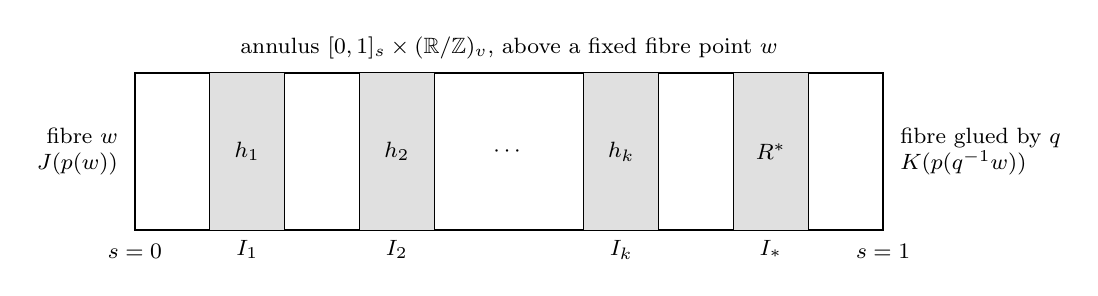
\begin{tikzpicture}[x=0.95cm,y=1cm,font=\footnotesize]
 \draw[thick] (0,0) rectangle (10,2);
 \foreach \l/\r/\t in {1/2/{h_1},3/4/{h_2},6/7/{h_k},8/9/{R^*}} {
  \fill[black!12] (\l,0) rectangle (\r,2);
  \draw (\l,0) -- (\l,2); \draw (\r,0) -- (\r,2);
  \node at ({(\l+\r)/2},1) {$\t$};
 }
 \node at (5,1) {$\cdots$};
 \node[below] at (1.5,0) {$I_1$}; \node[below] at (3.5,0) {$I_2$};
 \node[below] at (6.5,0) {$I_k$}; \node[below] at (8.5,0) {$I_*$};
 \node[below] at (0,-0.05) {$s=0$}; \node[below] at (10,-0.05) {$s=1$};
 \node[left,align=right] at (-0.1,1) {fibre $w$\\$J(p(w))$};
 \node[right,align=left] at (10.1,1) {fibre glued by $q$\\$K(p(q^{-1}w))$};
 \node[above] at (5,2.05) {annulus $[0,1]_s\times(\R/\Z)_v$, above a fixed fibre point $w$};
\end{tikzpicture}
\caption{The annulus above a fibre point $w$ in dimension four. The $\beta$-coefficient rises from $J(p(w))$ to
$K(p(q^{-1}w))$; across the layer $I_i$ it rises by the cap $h_i(p(w))$ of the $i$-th ball and across $I_*$ by the
positive remainder $R^*(w)$.}
\label{fig:mech-layers}
\end{figure}

The general comparator is constructed from a concave piecewise affine minorant $P$ with positive mean.
For its finite fixed-point construction choose
\begin{equation}\label{eq:mech-necessary}
 0<d<\min\bigl(\bar P,\beta_P\bigr),\qquad
 \bar P=|\Delta|^{-1}\int_\Delta P,
\end{equation}
where $P\ge\beta_P>0$ off the core $\tau_\Delta\Delta$. Section~\ref{sec:cmp} constructs $K$ and $q_t$ and accounts for
all approximation errors in the retained gap. The increasing rearrangements act on the moment
polytope, and their Hamiltonian realisations act on the fibres. For the equal-ball four-dimensional
case with $k\ge10$ and $\frac34<\rho\sqrt k<1$, the linear comparison of Proposition~\ref{prop:cmp-linear} gives the datum directly.

\subsection{Model, comparison datum and transfer}\label{sec:mech-interfaces}

\begin{definition}[Model input]\label{def:mech-model}
\lean{SymplecticPacking.HighDim.RawToricModel,
SymplecticPacking.HighDim.ToricPackingStages.smallRawModel,
SymplecticPacking.HighDim.ToricPackingStages.mixedRawModel,
SymplecticPacking.HighDim.ToricPackingStages.cubicRawTotalModel}
A higher-dimensional model input consists of a compact affine core $\Sigma_\ell\subset M$ of an affine
curve $M$, the product $E=M\times\C^m$, a downward polytope $\Delta$, and the physical primitive
$\Gamma_{\rm phys}(p)$ given in the corresponding model section, together with the handle data of
Definition~\ref{def:hdl-handle-data}. The physical form is
\[
 \Omega=\omega_V+d\Gamma_{\rm phys},\qquad
 V_\Delta(E)=\Sigma_\ell\times V_\Delta.
\]
The physical curvature $\kappa(p)=d_\Sigma\Gamma_{\rm phys}(p)$ is positive on the model region and extends
smoothly in the moment variables across the coordinate hyperplanes. The four-dimensional input is the
periodic cubic model of \Sref{Definition}{def:cub-model}; its maps are equivariant for the deck maps
given there.
\end{definition}

\begin{definition}[Comparison datum]\label{def:mech-datum}
\lean{SymplecticPacking.HighDim.ComparisonDatum,
SymplecticPacking.HighDim.ComparisonDatum.qMap,
SymplecticPacking.HighDim.CmpInput.comparatorDatum}
A comparison datum for $(\Delta,P)$ with gap $\gamma>0$ and reserve $\gamma_*\in(0,\gamma]$ consists of a function
$K$ of the moments, smooth on a neighbourhood of $\Delta$ in $\R^m$, and a smooth Hamiltonian isotopy
$(q_t)_{t\in[0,1]}$ of $\C^m$ with $q_0=\mathrm{id}$, generated by $Q_t$ with $\iota_{X_{Q_t}}\omega_V=-dQ_t$,
such that:
\begin{enumerate}[label=(\arabic*),ref=(\arabic*)]
\item\label{it:mech-datum-collar} $q_t(V_\Delta)=V_\Delta$ for every $t$, and there is $\varsigma>0$ such that
 for every face $\nu$ and every $t$, $Q_t$ Poisson-commutes with the face moment $\mu_\nu=\langle b_\nu,p\rangle$ on
 the collar $\{\mu_\nu>\ell_\nu-\varsigma\}$;
\item\label{it:mech-datum-cmp} $q=q_1$ satisfies the comparison inequality~\eqref{eq:mech-comparison}.
\end{enumerate}
For the comparator of Theorem~\ref{thm:cmp-main}, with gap $\gamma=\frac{11}{16}d$, the models take the reserve
$\gamma_*=\frac{11}{64}d$.
\end{definition}

\begin{definition}[Transfer]\label{def:mech-transfer}
\lean{SymplecticPacking.BranchSmall.vectorTransfer,
SymplecticPacking.BranchLargeHigh.Two.returnMap,
SymplecticPacking.BranchLarge3.RawTransfer.transferMap,
SymplecticPacking.Return.compositeT}
A transfer to an open target $U\subset\C^n$ assigns to a compact subset $\mathcal K$ of the model
domain a smooth symplectic embedding $\mathcal T_{\mathcal K}$ on a neighbourhood of $\mathcal K$,
and an explicit compact set $\mathcal C_{\mathcal K}\subset U$ containing the image of $\mathcal K$.
The cubic, quadric and six-dimensional polynomial transfers are fixed maps; in the shell transfer for
$n\ge4$ the slit-shell parameters depend on $\mathcal K$.
\end{definition}

\begin{theorem}[Packing in a model]\label{thm:mech-packing}
\lean{SymplecticPacking.HighDim.RawModelAgreement.native_packing_spec, SymplecticPacking.Strip.Cubic.fN_symplectic, SymplecticPacking.Strip.Cubic.fN_disjoint, SymplecticPacking.Strip.Cubic.fN_avoid_fibres}
Let $n\ge3$ and let $(\Sigma_\ell,\Delta,\Gamma_{\rm phys})$ be a model input
(Definition~\ref{def:mech-model}) whose handle data satisfy the collar bounds~\eqref{eq:hdl-collar}. Let
$(K,(q_t))$ be a comparison datum for $(\Delta,P)$ with gap $\gamma$ and reserve $\gamma_*$
(Definition~\ref{def:mech-datum}). Let $0<\rho_i<a_i$ $(1\le i\le k)$ with
$\{|p|\le a_i\}\subset\tau_\Delta\Delta$, and suppose
\[
 P(p)\le\Hb(p)-\sum_i(a_i-|p|)_+\qquad(p\in\Delta).
\]
Then the maps $\psi_i$ of \Sref{Construction}{cons:native-packing} are smooth symplectic embeddings of
neighbourhoods of the closed balls $B(\rho_i)$ into $(E,\Omega)$, and the sets $\psi_i(B(\rho_i))$ are pairwise
disjoint and contained in $\operatorname{int}V_\Delta(E)$. For $n=2$ the same conclusion holds for the cubic
model of \Sref{Definition}{def:cub-model} with the handle data of \Sref{Proposition}{prop:cub-handle} and the
equivariant maps of \Sref{Section}{sec:cub}, when the comparison datum is replaced by valid cubic data
(\Sref{Definition}{def:shd4-data}): the full-disc comparison for the profile itself and the collar condition
$P_{\rm supp}<h$.
\end{theorem}

The model sections verify the density floor, the collar bounds and the profile minorant before applying
this theorem; the proof is in \S\ref{sec:hdl-proof}.

\begin{proposition}[Assembly]\label{prop:mech-assembly}
\lean{OAI.PackingSufficiencySupport.Hamiltonian.postcompose_form_packing, SymplecticPacking.HighDim.assembly_spec}
Let $\psi_i$ be the model embeddings of Theorem~\ref{thm:mech-packing} and let $\mathcal T$ be its transfer.
Then, with $\mathcal K=\bigcup_i\psi_i(B(\rho_i))$, the maps
$f_i=\mathcal T_{\mathcal K}\circ\psi_i$ are smooth symplectic embeddings on neighbourhoods of
$B(\rho_i)$, have pairwise disjoint images in $U$, and have images contained in $\mathcal C_{\mathcal K}$.
\end{proposition}
\begin{proof}
The set $\mathcal K$ is compact, and the transfer is one injective symplectic map on a neighbourhood of
it, so composition preserves the pullback identity and disjointness. The inverse images of that
neighbourhood under the $\psi_i$ are open neighbourhoods of the source balls.
\end{proof}

\begin{table}[ht]
\centering\footnotesize
\renewcommand{\arraystretch}{1.2}
\begin{tabular}{@{}L{.16\textwidth}L{.24\textwidth}L{.25\textwidth}L{.25\textwidth}@{}}
\toprule
input & base and physical primitive & base profile & target\\\midrule
$n=2$ & disc bundle over the cubic, on its periodic cover & $3(1-3p)$ & $\Bo(1)$\\
$n\ge3$, all $c_i<C/2$ & $y_j^2=t^2-j$, $m=n-1$; $(1-2|p|)\lambda$ & $A_\ell(1-2|p|)$; limit $2^m(1-2|p|)$ & $\Bo(1)$\\
$n\ge4$, one large ball & same affine curve with $q=n-2$; $(1-u-2w)\lambda$ & $A_\ell(1-u-2w)$; limit $2^q(1-u-2w)$ & a shell about the reserved ball\\
$n=3$, one large ball & an explicit polynomial primitive on a compact affine core & $H_\ell$, limit $9(b-|p|)-2(s-|p|)_+$ & common polynomial form, then $\Bo(1)$\\\bottomrule
\end{tabular}
\caption{The four models. $A_\ell$ is the reference area of the compact affine core; each
higher-dimensional total space is a product over that core. The model sections give the heights,
truncation level and transfer parameters.}
\label{tab:mech-models}
\end{table}

\subsection{The scalar budget}\label{sec:mech-volume}

For a small-ball input define $\mathcal B_\Delta$ by \eqref{eq:mech-model-volume}. The cap identity gives
\begin{equation}\label{eq:mech-budget}
 \frac{1-\sum_i\rho_i^n}{n!}
 =\left(\frac1{n!}-\mathcal B_\Delta\right)
   +\int_\Delta\Pb
   +\sum_i\frac{a_i^n-\rho_i^n}{n!}.
\end{equation}
The model parameters make the sum of the first and last terms on the right smaller than the left side, so that
$\int_\Delta\Pb>0$. In the quadric input the reference-area tail controls the difference from the limiting affine
profile; in the six-dimensional input an explicit area modulus controls $H_\ell-H_0$, including the
additional two-level collar margin. The comparison operates on a minorant with positive mean and
positive values near the outer faces. Its reserve pays for the background and collar mass, and
$a_i-\rho_i$ pays for the strip and the source neighbourhood.

For a large-ball input the limiting budget for the remaining balls is $(1-a^n)/n!$, with $a$ the
reserved capacity; the shell parameters ($n\ge4$) or the polynomial profile ($n=3$) provide it. In all cases the
transfer is applied to the already constructed compact family of model images.

\begin{table}[ht]
\centering\footnotesize
\begin{tabular}{@{}ll@{}}
\toprule
symbol & meaning\\\midrule
$n$, $m=n-1$ & phase dimension and fibre rank\\
$p$, $|p|$, $\Delta$, $V_\Delta$ & fibre moments, their sum, moment polytope and toric domain\\
$\kappa$, $\Hb$, $\mathcal B_\Delta$ & physical base curvature, its intrinsic area and its moment budget\\
$P$, $K$, $q_t$, $\gamma$, $\gamma_*$ & profile minorant, comparison function, isotopy, gap and reserve\\
$H^*$, $J$, $h_i$, $R^*$ & normalised handle mass, $K-H^*$, smooth caps and residual\\
$\mathcal D$, $\Phi_j$, $\mathcal E_i$ & suspension, three Moser endpoints and layer maps\\
$\mathcal T_{\mathcal K}$ & transfer on the compact model images\\\bottomrule
\end{tabular}
\caption{Notation for the model and handle construction.}
\label{tab:mech-notation}
\end{table}

\section{Hamiltonian comparison}\label{sec:cmp}

This section produces the comparison data of Definition~\ref{def:mech-datum}. Let $\Delta$ be a compact
full-dimensional downward polytope with outer faces $\langle b_\nu,p\rangle\le\ell_\nu$ (\S\ref{sec:mech-interfaces}),
let $V_\Delta=\{w\in\C^m:p(w)\in\Delta\}$ be its toric domain, with $p_j=\pi|w_j|^2$, $\theta_j=\arg w_j/2\pi\in\R/\Z$
and $\omega_V=\sum_jdp_j\wedge d\theta_j$ as in \S\ref{sec:mech}, and let $P$ be a continuous concave function on $\Delta$
with positive mean; in the general construction $P$ is rational concave piecewise affine and positive off a core
$\tau_\Delta\Delta$. We seek a smooth toric function $K$ and a Hamiltonian isotopy $q_t$ of $V_\Delta$ with
$(K-P)\circ p\circ q_1\le K\circ p-\gamma$ for some $\gamma>0$. Since $q_1$ preserves the measure $\omega_V^m/m!$ and,
the angles having period $1$, $p_*(\omega_V^m/m!)$ is Lebesgue measure on $\Delta$, the map $q_1$ can only redistribute
the values of $K-P$; the inequality asks that after redistribution they lie below $K-\gamma$. The construction has
two halves: a scalar half (rearrangement operators on convex functions on $\Delta$ and a contraction whose
approximate fixed point is $K$, \S\S\ref{sec:cmp-rearrangement}--\ref{sec:cmp-fixed}) and a symplectic half
(isotopies realising one coordinate rearrangement up to a prescribed error, \S\ref{sec:cmp-realisation}).

The rearrangement operator and the contraction are those of \cite[\S2]{OpenAI2026}. We replace the fixed point by a
finite rational iterate with explicit iteration count and gap (Proposition~\ref{prop:cmp-fixed-point}), and the
existence of realising isotopies by explicit Hamiltonians (Theorem~\ref{thm:cmp-realisation}). For $k\ge10$ equal
balls in dimension four with $\frac34<\rho\sqrt k<1$ no fixed point is needed: $K$ is linear, the rearranged inequality
is an identity, and the inner planar map costs at most $g/32$ of the gap (\S\ref{sec:cmp-linear}). Every object defined in this section is explicit at level L1
(Definition~\ref{def:intro-levels}).

The polyhedral iterate with log-sum-exp smoothing (Theorem~\ref{thm:cmp-main}) is used for all
higher-dimensional models. The general four-dimensional case uses the scalar version of \Ssec{sec:scalar-cmp}, in
which the finite iterate is extended by an infimal formula and smoothed by convolution with a fixed bump; its gap
and its planar Hamiltonian are \Sref{Proposition}{prop:scalar-cmp-gap} and
\Sref{Proposition}{prop:scalar-planar-realisation}. The four-dimensional equal-ball case with $k\ge10$ uses the linear
datum of \S\ref{sec:cmp-linear}.

Throughout, fibre Hamiltonians follow the convention $\iota_{X_Q}\omega_V=-dQ$ of
Definition~\ref{def:mech-datum}. Norms $\|\cdot\|$ are uniform norms on $\Delta$. For a coordinate $j$ we write
$p=(y,x)$ with $x=p_j$ and $y=(p_i)_{i\ne j}$. The polytope $\Delta$ is \emph{rational} if all $b_\nu,\ell_\nu$ are
rational. A function on $\Delta$ is \emph{rational convex polyhedral} if it is the restriction to $\Delta$ of
$\max_{\iota\in I}\phi_\iota$ for a finite family of affine functions $\phi_\iota$ with rational coefficients, and
\emph{rational concave piecewise affine} if it is $\min_{\iota\in I}\phi_\iota$ for such a family. All cutoffs and
clocks below use the flat step $S$ of \Sref{Definition}{def:pre-flat}, all of whose derivatives vanish at $0$ and
$1$.

\subsection{Coordinate rearrangement}\label{sec:cmp-rearrangement}

Fix $j$. Because every $b_\nu$ is nonnegative and $\Delta$ is compact, at least one $\nu$ has $b_{\nu j}>0$, and
\[
 L(y)=\min_{\nu:\,b_{\nu j}>0}\frac{\ell_\nu-\sum_{i\ne j}b_{\nu i}y_i}{b_{\nu j}}
\]
is a continuous concave piecewise affine function on the projection $\Delta_j=\{y:(y,0)\in\Delta\}$, with
$\Delta=\{(y,x):y\in\Delta_j,\ 0\le x\le L(y)\}$. The slice of $\Delta$ through $y$ is the interval $[0,L(y)]$.

\begin{definition}[Coordinate rearrangement]\label{def:cmp-rearrangement}
For a continuous convex function $F$ on $\Delta$ and a coordinate $j$, put
\[
 (R_jF)(y,x)=\min_{\substack{0\le a,\ a+x\le L(y)}}\ \max\bigl(F(y,a),\,F(y,a+x)\bigr),
 \qquad (y,x)\in\Delta,
\]
and $\Rcal=R_m\circ\dots\circ R_1$.
\end{definition}

The minimum exists because the admissible $a$ form the compact interval $[0,L(y)-x]$. Since the sublevel sets of
a convex function of one variable are intervals, $x\mapsto(R_jF)(y,x)$ is the increasing rearrangement of
$F(y,\cdot)$ on $[0,L(y)]$ with respect to Lebesgue measure: for $x>0$ it is the smallest value $b$ for which
$\{F(y,\cdot)\le b\}$ has length at least $x$; at $x=0$ it equals $\min F(y,\cdot)$.

\begin{lemma}[Properties of $R_j$]\label{lem:cmp-rearrangement}
\uses{def:cmp-rearrangement, S-lem:fcp-rearrangement, S-lem:fcp-polyhedral}
Let $F,G$ be continuous convex functions on $\Delta$ and $j\in\{1,\dots,m\}$.
\begin{enumerate}[label=(\roman*)]
\item $R_jF$ is continuous and convex on $\Delta$, and $\int_\Delta R_jF=\int_\Delta F$.
\item If $F\le G$ then $R_jF\le R_jG$; $R_j(F+c)=R_jF+c$ and $R_j(\alpha F)=\alpha R_jF$ for constants $c\in\R$,
 $\alpha\ge0$; $\|R_jF-R_jG\|\le\|F-G\|$.
\item For each $y$, $x\mapsto(R_jF)(y,x)$ is nondecreasing, $(R_jF)(y,0)=\min_{[0,L(y)]}F(y,\cdot)$ and
 $(R_jF)(y,L(y))=\max_{[0,L(y)]}F(y,\cdot)$; in particular $\max_\Delta R_jF=\max_\Delta F$.
\item If $F$ is nondecreasing in $p_i$ for some $i\ne j$, so is $R_jF$. Consequently $\Rcal F$ is
 nondecreasing in every coordinate, and $\Rcal F(0)=\min_\Delta\Rcal F$.
\item Let $\Delta$ be rational. If $F$ is rational convex polyhedral, so is $R_jF$. If $F=\max_{\iota\in I}\phi_\iota$,
 the epigraph of $R_jF$ over $\Delta$ is the projection to $(y,x,t)$ of the rational polyhedron in the variables
 $(y,x,t,a)$ defined by $p=(y,x)\in\Delta$, $a\ge0$, $b_{\nu j}(a+x)+\sum_{i\ne j}b_{\nu i}y_i\le\ell_\nu$ for every
 $\nu$ with $b_{\nu j}>0$, and $t\ge\phi_\iota(y,a)$, $t\ge\phi_\iota(y,a+x)$ for every $\iota\in I$; eliminating $a$
 by Fourier--Motzkin elimination gives finitely many rational affine functions whose maximum is $R_jF$.
\end{enumerate}
\end{lemma}

\begin{proof}
The proofs are in \Sref{Lemma}{lem:fcp-rearrangement} and \Sref{Lemma}{lem:fcp-polyhedral}; we give the arguments
for convexity, monotonicity and (v). Convexity: if $[a_0,a_0+x_0]$ and $[a_1,a_1+x_1]$ are minimising intervals on
the slices through $y_0$ and $y_1$, their convex combination with weights $1-\vartheta,\vartheta$ is admissible on the
slice through $(1-\vartheta)y_0+\vartheta y_1$ (concavity of $L$), and convexity of $F$ bounds its endpoint values by
the corresponding convex combinations. Monotonicity in $p_i$: lowering $y_i$ does not shrink the slice, because
$b_{\nu i}\ge0$, so every admissible interval stays admissible while its endpoint values do not increase. Item (v):
the minimum in Definition~\ref{def:cmp-rearrangement} is attained, so $t\ge R_jF(y,x)$ if and only if some $a$
satisfies the displayed system, and the epigraph is the projection. The variable $t$ occurs only in lower bounds
$t\ge\dots$, and Fourier--Motzkin elimination of $a$ forms nonnegative combinations of the given inequalities; so it
produces only inequalities of the form $t\ge$ (affine function of $(y,x)$) and inequalities free of $t$. The latter
hold on $\Delta$, because every $(y,x)\in\Delta$ has a feasible $a$ (for instance $a=0$, with $t$ large), and hence
$R_jF$ is the maximum of the former.
\end{proof}

\subsection{A finite comparator iteration}\label{sec:cmp-fixed}

For $0<\lambda<1$ consider $T_\lambda(F)=\Rcal(\lambda F-P)$ on the space of continuous convex functions on $\Delta$.
If $P$ is concave, $\lambda F-P$ is convex, and by Lemma~\ref{lem:cmp-rearrangement}(ii) $T_\lambda$ is a
contraction with constant $\lambda$.

\begin{proposition}[Finite comparator]\label{prop:cmp-fixed-point}
\uses{lem:cmp-rearrangement, S-prop:fcp-fixed-point}
Let $\Delta$ be rational, $\tau_\Delta\in(0,1)$ rational, and $P$ a rational concave piecewise affine function on
$\Delta$ with mean $\mu=\vol(\Delta)^{-1}\int_\Delta P>0$ and $P\ge\beta_P$ on $\Delta\setminus\tau_\Delta\Delta$ for some
$\beta_P>0$. Let $d$ be rational with $0<d<\min(\mu,\beta_P)$ and put
\[
 \eta_\Delta=(1-\tau_\Delta)(\mu-d),\qquad M_P=\max\bigl(1,\ d-\min_\Delta P+1\bigr),\qquad
 \lambda=1-\frac{\eta_\Delta}{2(M_P+\eta_\Delta)}.
\]
Define $K_0=0$, $K_{r+1}=\Rcal(\lambda K_r-P)$ and
\[
 N=\left\lceil\frac{16\|P\|}{d(1-\lambda)(\lambda^{-1}-1)}\right\rceil+1.
\]
Then every $K_r$ is rational convex polyhedral, $\lambda^N\|P\|/(1-\lambda)<d/16$, and
\[
 \Rcal(K_N-P)\le K_N-\tfrac78d\qquad\text{on }\Delta .
\]
\end{proposition}

All quantities in Proposition~\ref{prop:cmp-fixed-point} are computed by finite rational arithmetic. For a
rational convex polyhedral $G$, Lemma~\ref{lem:cmp-rearrangement}(iii),(iv) give $\min_\Delta G=(\Rcal G)(0)$, and
the maximum of an affine function $\phi$ is $-\min_\Delta(-\phi)$; this gives $\min_\Delta P$ and $\|P\|$ by
Fourier--Motzkin elimination. The integral $\int_\Delta P$, hence $\mu$, is computed by iterated integration of
rational polynomials over rational polyhedral cells, one coordinate at a time
(\Sref{Proposition}{prop:fcp-fixed-point}(a)). Hence $N$ is obtained by rational arithmetic and a ceiling, and
$K_N$ by $mN$ Fourier--Motzkin eliminations (Lemma~\ref{lem:cmp-rearrangement}(v)).

\begin{proof}
\emph{Rationality.} $K_0=0$, and if $K_r=\max_\iota\phi_\iota$ and $P=\min_u\psi_u$ with rational affine
$\phi_\iota,\psi_u$, then $\lambda K_r-P=\max_{\iota,u}(\lambda\phi_\iota-\psi_u)$ is rational convex polyhedral, so
$K_{r+1}$ is by Lemma~\ref{lem:cmp-rearrangement}(v) applied $m$ times.

\emph{The fixed point.} The continuous convex functions on $\Delta$ form a closed subset of $C(\Delta)$, so the
$\lambda$-contraction $T_\lambda$ has a unique fixed point $K_\lambda$ (the comparison function of
\cite[\S2.2]{OpenAI2026}), and $\|K_r-K_\lambda\|\le\lambda^r\|K_\lambda\|$. Since $\Rcal0=0$ and $\Rcal$ is
$1$-Lipschitz, $\|K_\lambda\|\le\lambda\|K_\lambda\|+\|P\|$, so $\|K_\lambda\|\le\|P\|/(1-\lambda)$. By
Lemma~\ref{lem:cmp-rearrangement}(i),(iv), $K_\lambda$ is convex, nondecreasing in every coordinate,
$K_\lambda(0)=\min K_\lambda$, and integrating the fixed-point equation gives
$\int K_\lambda=\lambda\int K_\lambda-\int P$, that is, the mean of $K_\lambda$ is $-\mu/(1-\lambda)$.

\emph{The gap of the fixed point.} Note $\tfrac12<\lambda<1$, $1-\lambda=\eta_\Delta/(2(M_P+\eta_\Delta))$ and
\begin{equation}\label{eq:cmp-lambda}
 \frac{\lambda\eta_\Delta}{1-\lambda}=2M_P+\eta_\Delta>d-\min_\Delta P .
\end{equation}
The idea is that the mean of $K_\lambda$ is very negative, so by convexity its values on the core
$\tau_\Delta\Delta$ lie well below its maximum, while off the core $P\ge\beta_P$ lowers $\lambda K_\lambda-P$; the
fixed-point equation then forces the maximum of $K_\lambda$ to be negative. In detail, let $M_\lambda=\max K_\lambda$ and suppose $M_\lambda\ge-d/(1-\lambda)$, so that
$\lambda M_\lambda\le M_\lambda+d$. If $p\in\Delta\setminus\tau_\Delta\Delta$, then
$\lambda K_\lambda(p)-P(p)\le\lambda M_\lambda-\beta_P<M_\lambda$, because $(1-\lambda)M_\lambda\ge-d>-\beta_P$. If
$p=\tau_\Delta v$ with $v\in\Delta$, convexity and $K_\lambda(0)=\min K_\lambda\le-\mu/(1-\lambda)$ give
\[
 K_\lambda(p)\le\tau_\Delta M_\lambda+(1-\tau_\Delta)K_\lambda(0)
 \le M_\lambda-(1-\tau_\Delta)\Bigl(M_\lambda+\frac{\mu}{1-\lambda}\Bigr)\le M_\lambda-\frac{\eta_\Delta}{1-\lambda},
\]
the last step by $M_\lambda\ge-d/(1-\lambda)$. Hence, by \eqref{eq:cmp-lambda},
\[
 \lambda K_\lambda(p)-P(p)\le M_\lambda+d-\frac{\lambda\eta_\Delta}{1-\lambda}-\min_\Delta P<M_\lambda .
\]
Thus $\max_\Delta(\lambda K_\lambda-P)<M_\lambda$, while Lemma~\ref{lem:cmp-rearrangement}(iii) and the fixed-point
equation give $M_\lambda=\max\Rcal(\lambda K_\lambda-P)=\max(\lambda K_\lambda-P)$, a contradiction. Therefore
$M_\lambda<-d/(1-\lambda)$, i.e.\ $(1-\lambda)K_\lambda<-d$ on $\Delta$, and by Lemma~\ref{lem:cmp-rearrangement}(ii)
\[
 \Rcal(K_\lambda-P)=\Rcal\bigl(\lambda K_\lambda-P+(1-\lambda)K_\lambda\bigr)\le\Rcal(\lambda K_\lambda-P)-d=K_\lambda-d .
\]

\emph{The finite iterate.} Let $r_N=\|K_N-K_\lambda\|\le\lambda^N\|P\|/(1-\lambda)<d/16$. By
Lemma~\ref{lem:cmp-rearrangement}(ii),
$\Rcal(K_N-P)\le\Rcal(K_\lambda-P)+r_N\le K_\lambda-d+r_N\le K_N-d+2r_N<K_N-\tfrac78d$.
\end{proof}

The construction applies verbatim when the polytope and the affine pieces have real coefficients:
Fourier--Motzkin elimination uses finitely many arithmetic operations and comparisons, and the estimates are
unchanged, with ``rational convex polyhedral'' replaced by ``convex polyhedral''. The same holds for the smoothing
and realisation statements below. This real version is the one used for real capacities.

\subsection{Realisation and the comparison datum}\label{sec:cmp-realisation}

The symplectic half realises one coordinate rearrangement by an isotopy which changes only the $j$-th
moment; the other fibre coordinates may rotate.

\begin{theorem}[Realisation of one coordinate rearrangement]\label{thm:cmp-realisation}
\lean[needed]{SymplecticPacking.HighDim.liftGen_spec}
\uses{lem:cmp-rearrangement, S-def:plc-slice, S-thm:plc-lift, S-thm:pln-isotopy}
Let $\Delta$ be rational, $F$ rational convex polyhedral on $\Delta$, $j\in\{1,\dots,m\}$ and $e>0$ rational. Let
$Q^{(j)}_t$ be the Hamiltonian defined from $(\Delta,F,j,e)$ in \Sref{Definition}{def:plc-slice}, and let
$(q^{(j)}_t)_{t\in[0,1]}$ be its flow ($\iota_{X}\omega_V=-dQ^{(j)}_t$). Then $Q^{(j)}$ is smooth with compact support
in $w$, $(q^{(j)}_t)$ is a smooth Hamiltonian isotopy of $\C^m$, and:
\begin{enumerate}[label=(\alph*)]
\item $q^{(j)}_0=\mathrm{id}$; every $q^{(j)}_t$ maps $V_\Delta$ onto itself and preserves the moments $p_i$, $i\ne j$.
\item There is a rational $\varsigma_j>0$ such that for every $\nu$ with $b_{\nu j}>0$ and every $t$, $Q^{(j)}_t$
 vanishes on $\{\langle b_\nu,p\rangle>\ell_\nu-\varsigma_j\}$; for every $\nu$ with $b_{\nu j}=0$, $Q^{(j)}_t$
 Poisson-commutes with $\langle b_\nu,p\rangle$.
\item $F\bigl(p(q^{(j)}_1(w))\bigr)\le(R_jF)(p(w))+e$ for every $w\in V_\Delta$.
\end{enumerate}
\end{theorem}

The proof is \Sref{Theorem}{thm:plc-lift}. The theorem enters through Theorem~\ref{thm:cmp-main}, which is used for
$2n\ge6$; the general four-dimensional branch realises its single rearrangement by the planar path of
\Sref{Proposition}{prop:scalar-planar-realisation} instead. The construction is planar and rests on the following fact: if
$f$ is a convex function on $[0,1]$ and $f^\sharp$ its increasing rearrangement, there are area-preserving maps
$q$ of the disc of area $1$ with $f(\pi|q(z)|^2)\le f^\sharp(\pi|z|^2)+\xi$ for any $\xi>0$. Such a map carries
each disc $\{\pi|z|^2\le I\}$ onto a region of area $I$ on which $f(\pi|\cdot|^2)\le f^\sharp(I)+\xi$. In the
moment--angle rectangle $(0,1)\times(-\frac12,\frac12)$, with area form $dv\wedge d\theta$, we take these regions to
be the sublevel sets of one convex potential that approximates $f(v)$ and is proper in the angle, and build the map
from its level curves.

In detail, fix $y$ and rescale the inner slice $[0,\ell_{\rm in}(y)]$ to $[0,1]$, where $\ell_{\rm in}(y)<L(y)$
is a smooth inner slice length. Then $f(v)=F(y,\ell_{\rm in}(y)v)$ is convex on $[0,1]$ with increasing
rearrangement $f^\sharp$, and we need $q_{\rm in}$ with the displayed inequality on a core disc, with planar
error $\xi=e/4$. Smooth $f$ by log-sum-exp and add the barrier $\kappa_0(1/v+1/(1-v))$ with a small positive
$\kappa_0$; this gives a real-analytic, strictly convex, proper potential $U$ on $(0,1)$. Add to it a small
multiple of the proper even wall $\theta^2/(\frac14-\theta^2)$ in the angle. The sublevel sets of the sum are
nested ovals in the rectangle, and the level enclosing area $I$ lies below $f^\sharp(I)$ plus a small error
(\Sref{Lemma}{lem:plc-area}). To compare these ovals with round circles we make the potential exactly quadratic
near its minimum: the two one-variable wells are modified on small intervals, with error at most $\xi/64$ each
(\Sref{Lemma}{lem:plc-modified-area}). In the signed square roots of the two wells the sum is then the squared
radius, so after a rotation and a normalisation of area the centred circle enclosing area $I$ is carried onto the
level of the modified potential enclosing area $I$. The chart $(v,\theta)\mapsto-\sqrt{v/\pi}\,e^{2\pi i\theta}$,
in which $dv\wedge d\theta$ is the area form, returns to the disc (\Sref{Theorem}{thm:pln-inner}).

A compactly supported Hamiltonian isotopy of the disc ends at $q_{\rm in}$ on a core disc whose complement has area
exactly $8\eta$, with $\eta=\tfrac12\min(1/16,\xi/[32(\Lambda_f+1)])$, where $\Lambda_f\ge1$ bounds the slopes of
$f$ (\Sref{Theorem}{thm:pln-isotopy}); outside the core, Lipschitz continuity of $f^\sharp$ gives
\[
 f\le\max f=f^\sharp(1)\le f^\sharp(\pi|z|^2)+8\Lambda_f\eta
 <f^\sharp(\pi|z|^2)+\xi.
\]
All constants are chosen uniformly in $y$ over an open parameter domain (\Sref{Theorem}{thm:plc-param}). The planar
generator is lifted as
\[
 Q^{(j)}_t(w)=\chi(y)S'(t)\ell_{\rm in}(y)\,
 Q^{\rm pl}\bigl(y,\chi(y)S(t),w_j/\sqrt{\ell_{\rm in}(y)}\bigr),
\]
with a cutoff
$\chi(y)$ vanishing near degenerate slices. The planar Hamiltonian is supported in $\{\pi|u|^2<r_B\}$ with $r_B<1$,
and $\ell_{\rm in}>\eta_1$ wherever $\chi\ne0$; this gives the positive real collar
$c_j=\frac12(1-r_B)\eta_1\min_{\nu:\,b_{\nu j}>0}b_{\nu j}$. The rational collar in (b) is $\varsigma_j=2^{-N_j}$ with $N_j$ the least natural number such that $2^{-N_j}<c_j$;
this choice does not affect the Hamiltonian. The lifted motion fixes every point with
$p_j\ge r_B\ell_{\rm in}(y)$, and $\ell_{\rm in}<L$, so every slice $\{y\}\times[0,L(y)]$ is preserved. The general convex
construction is \Ssec{sec:plc}; the equal-ball instance, in which the potential is the tent of \S\ref{sec:cmp-linear},
is \Ssec{sec:pll}; the common planar machinery is \Ssec{sec:pln}.

\begin{theorem}[Comparison datum for concave profiles]\label{thm:cmp-main}
\uses{prop:cmp-fixed-point, thm:cmp-realisation, def:mech-datum, S-lem:fcp-smoothing}
Assume the hypotheses of Proposition~\ref{prop:cmp-fixed-point}, and let $d$, $N$ and $K_N$ be as there. Let
$K_N=\max_{\iota\in I}\phi_\iota$ be the representation by rational affine functions produced by the iteration, each
step $R_j$ being the Fourier--Motzkin elimination of Lemma~\ref{lem:cmp-rearrangement}(v), set
$c_K=\lceil32\,\#I/d\rceil+1$ (so that $\log(\#I)/c_K<d/32$ by \Sref{Lemma}{lem:fcp-smoothing}), and put
\[
 K=\frac1{c_K}\log\sum_{\iota\in I}e^{c_K\phi_\iota}.
\]
Let $F_0=K_N-P$ and $F_j=R_jF_{j-1}$ ($1\le j\le m$); let $q^{(j)}_t$ be the isotopy of
Theorem~\ref{thm:cmp-realisation} for $F_{j-1}$, the coordinate $j$ and $e_j=d/(8(m+1))$. Define $q_t$ by running
$q^{(m)},q^{(m-1)},\dots,q^{(1)}$ in turn with flat clocks: for $t\in[\frac{r-1}m,\frac rm]$, $r=1,\dots,m$, and
$j=m+1-r$,
\[
 q_t=q^{(j)}_{S(mt-r+1)}\circ q^{(j+1)}_1\circ\dots\circ q^{(m)}_1 .
\]
Then $(K,(q_t))$ is a comparison datum for $(\Delta,P)$ with gap $\gamma=\tfrac{11}{16}d$.
\end{theorem}

\begin{proof}
The two expressions for $q_t$ at $t=r/m$ agree, so $q_t$ is well defined, $q_0=\mathrm{id}$ and
$q_1=q^{(1)}_1\circ\dots\circ q^{(m)}_1$. On $[\frac{r-1}m,\frac rm]$ the isotopy is generated by
$Q_t=mS'(mt-r+1)\,Q^{(j)}_{S(mt-r+1)}$, since precomposition with the fixed map
$q^{(j+1)}_1\circ\dots\circ q^{(m)}_1$ does not change the generating vector field. All derivatives of $S$ vanish at
$0$ and $1$, so $Q_t$ and $q_t$ are smooth in $t$ across the seams. Each factor maps $V_\Delta$ onto itself, so $q_t$
preserves $V_\Delta$. With $\varsigma=\min_j\varsigma_j$, Theorem~\ref{thm:cmp-realisation}(b) shows that every $Q_t$
Poisson-commutes with $\langle b_\nu,p\rangle$ on $\{\langle b_\nu,p\rangle>\ell_\nu-\varsigma\}$ for every $\nu$. This is
condition~\ref{it:mech-datum-collar} of Definition~\ref{def:mech-datum}.

For condition~\ref{it:mech-datum-cmp}, each $F_j$ is rational convex polyhedral by Lemma~\ref{lem:cmp-rearrangement}(v), so
Theorem~\ref{thm:cmp-realisation} applies, and $F_m=\Rcal(K_N-P)\le K_N-\tfrac78d$ by
Proposition~\ref{prop:cmp-fixed-point}. Fix $w\in V_\Delta$ and put $u_m=w$, $u_{j-1}=q^{(j)}_1(u_j)$, so that
$u_0=q_1(w)$ and all $u_j\in V_\Delta$. Theorem~\ref{thm:cmp-realisation}(c) gives
$F_{j-1}(p(u_{j-1}))\le F_j(p(u_j))+e_j$, and summing over $j$,
\[
 (K_N-P)\bigl(p(q_1(w))\bigr)\le F_m(p(w))+\sum_je_j\le K_N(p(w))-\tfrac78d+\tfrac18d=K_N(p(w))-\tfrac34d .
\]
For log-sum-exp, $\max_\iota\phi_\iota\le K\le\max_\iota\phi_\iota+\log(\#I)/c_K$, so $K_N\le K<K_N+d/32$ on $\R^m$
(\Sref{Lemma}{lem:fcp-smoothing}). Therefore
\[
 (K-P)\bigl(p(q_1(w))\bigr)<(K_N-P)\bigl(p(q_1(w))\bigr)+\tfrac{d}{32}\le K(p(w))-\tfrac34d+\tfrac1{32}d
 <K(p(w))-\tfrac{11}{16}d .
\]
$K$ is real-analytic on $\R^m$, hence smooth near $\Delta$, as Definition~\ref{def:mech-datum} requires.
\end{proof}

\subsection{The closed-form datum for equal balls}\label{sec:cmp-linear}

For $k\ge10$ equal capacities in dimension four the profile has a single kink, and the fixed point can be written
down: $K$ is linear and $K-P$ is, up to a constant, a tent whose increasing rearrangement is linear. This datum is
used in the equal-capacity branch of \Sref{Theorem}{thm:cub-packing}; Remark~\ref{rem:cmp-small-k} treats $k\le9$. Here
$m=1$, $\Delta=[0,h]$ with $h$ real (rationality is not used in this subsection), and $V_\Delta$ is the closed disc
$\bar D(h)$ of area $h$. The symbols $s,a,c_s,g,A,B$ below are local to this subsection and to
\Ssec{sec:fcp-equal}.

Let $k\ge10$ be an integer and $\eta_\star\in(0,\frac14)$, set $t_0=1-\eta_\star/2$, and put
\[
 s=\sqrt k,\quad a=\frac{t_0}s,\quad h=\frac{t_0}3,\quad c_s=3s-9,\quad g=3(1-t_0),\quad A=\frac ha,\quad B=\frac h{h-a}.
\]
Since $s>3$ we have $0<a<h$, $c_s>0$, $A,B>0$ and
\begin{equation}\label{eq:cmp-AB}
 \frac1A+\frac1B=\frac ah+\frac{h-a}h=1 .
\end{equation}
Define $\Lambda(x)=A(a-x)$ for $x\le a$ and $\Lambda(x)=B(x-a)$ for $x\ge a$. On $[0,h]$, $\Lambda$ is a tent with
$\Lambda(0)=\Lambda(h)=h$ and $\Lambda(a)=0$.

\begin{lemma}[Sublevel sets of the tent]\label{lem:cmp-tent-sublevel}
\lean{SymplecticPacking.Params.Rcal_le_iff, SymplecticPacking.Params.sublevel_length,
SymplecticPacking.Params.sublevel_subset, SymplecticPacking.Params.volume_sublevel}
\uses{eq:cmp-AB}
For $b\ge0$, $\{x\in\R:\Lambda(x)\le b\}=[a-b/A,\,a+b/B]$, an interval of length $b$. If $b\le h$, it is
contained in $[0,h]$.
\end{lemma}

\begin{proof}
The interval is read off from the two affine pieces; its length is $b(1/A+1/B)=b$ by \eqref{eq:cmp-AB}. If $b\le h$,
then $a-b/A\ge a-h/A=0$ and $a+b/B\le a+h/B=h$.
\end{proof}

\begin{corollary}[Rearrangement of the tent]\label{thm:cmp-tent-rearrangement}
\uses{lem:cmp-tent-sublevel, def:cmp-rearrangement}
With $m=1$ and $\Delta=[0,h]$, $R_1\Lambda(x)=x$ for $0\le x\le h$. Consequently
$R_1(-g+c_s\Lambda)(x)=-g+c_sx$.
\end{corollary}

\begin{proof}
For $\alpha=a-x/A$ we have $\alpha\ge0$, $\alpha+x=a+x/B\le h$ and $\Lambda(\alpha)=\Lambda(\alpha+x)=x$, so
$R_1\Lambda(x)\le x$. Conversely, if an admissible interval $[\alpha,\alpha+x]$ had
$b'=\max(\Lambda(\alpha),\Lambda(\alpha+x))<x$, then by convexity $[\alpha,\alpha+x]\subset\{\Lambda\le b'\}$, an
interval of length $b'<x$ by Lemma~\ref{lem:cmp-tent-sublevel}; this is impossible. The second statement follows
from Lemma~\ref{lem:cmp-rearrangement}(ii), since $c_s>0$.
\end{proof}

\begin{figure}[ht]
\centering
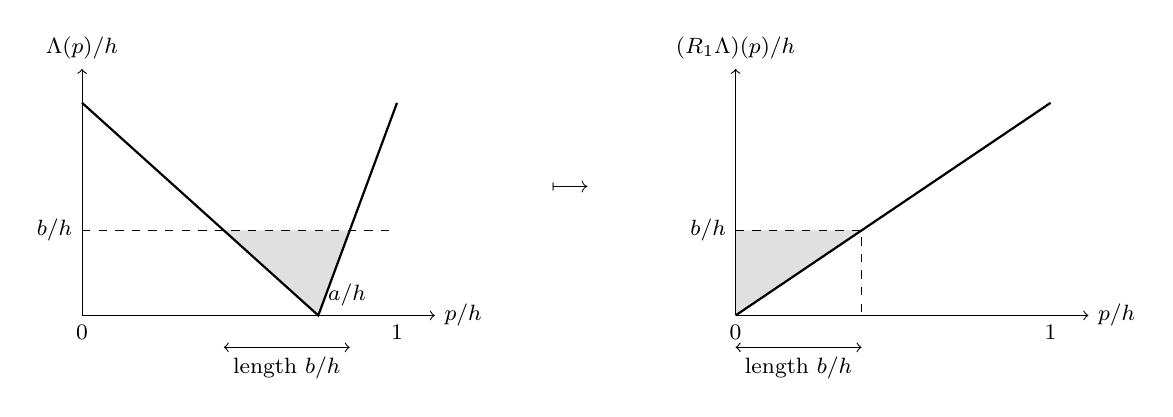
\begin{tikzpicture}[x=4cm,y=2.7cm,font=\footnotesize]
 \begin{scope}
 \fill[black!12] (0.45,0.4) -- (0.75,0) -- (0.85,0.4) -- cycle;
  \draw[->] (0,0) -- (1.12,0) node[right] {$p/h$};
  \draw[->] (0,0) -- (0,1.16) node[above] {$\Lambda(p)/h$};
  \draw[thick] (0,1) -- (0.75,0) -- (1,1);
  \draw[dashed] (0,0.4) node[left] {$b/h$} -- (1,0.4);
  \draw[<->] (0.45,-0.15) -- (0.85,-0.15) node[midway,below] {length $b/h$};
  \node[below] at (0,0) {$0$};
  \node[below] at (1,0) {$1$};
  \node[above right] at (0.75,0) {$a/h$};
 \end{scope}
 \node at (1.55,0.6) {$\longmapsto$};
 \begin{scope}[xshift=8.3cm]
  \fill[black!12] (0,0) -- (0,0.4) -- (0.4,0.4) -- cycle;
  \draw[->] (0,0) -- (1.12,0) node[right] {$p/h$};
  \draw[->] (0,0) -- (0,1.16) node[above] {$(R_1\Lambda)(p)/h$};
  \draw[thick] (0,0) -- (1,1);
  \draw[dashed] (0,0.4) node[left] {$b/h$} -- (0.4,0.4) -- (0.4,0);
  \draw[<->] (0,-0.15) -- (0.4,-0.15) node[midway,below] {length $b/h$};
  \node[below] at (0,0) {$0$};
  \node[below] at (1,0) {$1$};
 \end{scope}
\end{tikzpicture}
\caption{The linear comparison: the sublevel interval of $\Lambda$ has length $b$, so its increasing rearrangement
is $p$. The drawing uses $a/h=3/4$ ($k=16$); the identity holds for every $k\ge10$.
Consequently $K-R_1(K-P)\equiv g$, before the planar realisation error is deducted.}
\label{fig:cmp-tent}
\end{figure}

\begin{proposition}[Linear comparison datum for equal balls]\label{prop:cmp-linear}
\lean{SymplecticPacking.Params.F_eq, SymplecticPacking.Params.margin_one,
SymplecticPacking.Params.K_sub_F_ge, SymplecticPacking.Qhat.K_sub_F_q_ge,
SymplecticPacking.Qhat.full_comparison, SymplecticPacking.Qhat.qhatP_spec,
SymplecticPacking.Branch2.CubicData.ofParams_valid}
\uses{lem:cmp-tent-sublevel, thm:cmp-tent-rearrangement, def:mech-datum, S-lem:fcp-AB, S-def:fcp-eq, S-thm:pll-inner}
With the notation above let $\Delta=[0,h]$, $P(p)=3(1-3p)-k(a-p)_+$, $K(p)=c_sp$ and $F=K-P$. Then
\begin{equation}\label{eq:cmp-identity}
 F(x)=-g+c_s\Lambda(x)\qquad(x\in\R).
\end{equation}
Let $e_q=\min\bigl(h/100,\ g/(128c_s)\bigr)$ (\Sref{Definition}{def:fcp-eq}) and let $(q_t)$ be the isotopy of
\Sref{Theorem}{thm:pll-inner}, whose endpoint $q=q_1$ satisfies $\Lambda(p(q(z)))\le\pi|z|^2+4e_q$ on $\bar D(h)$.
Then $(K,(q_t))$ is a comparison datum for $(\Delta,P)$ with gap $\tfrac{31}{32}g$.
\end{proposition}

\begin{proof}
By \Sref{Lemma}{lem:fcp-AB}, $c_sA=k-3s$, $c_sB=3s$ and $3sa=3-g$. For $x\le a$:
$F(x)=c_sx-3+9x+k(a-x)=(3s-k)x+ka-3$, and $-g+c_sA(a-x)=(3s-k)x+ka-(g+3sa)=(3s-k)x+ka-3$. For $x\ge a$:
$F(x)=c_sx-3+9x=3sx-3$, and $-g+c_sB(x-a)=3sx-g-3sa=3sx-3$. This proves \eqref{eq:cmp-identity}.

By \Sref{Theorem}{thm:pll-inner}, $q_0=\mathrm{id}$, every $q_t$ maps $\bar D(h)$ onto itself and is the identity on
$\{\pi|z|^2>P_{\rm supp}\}$ for a constant $P_{\rm supp}<h$ defined there, and the generator $Q_t$ vanishes there; this
is condition~\ref{it:mech-datum-collar} of Definition~\ref{def:mech-datum} for the single outer face $p=h$. For condition~\ref{it:mech-datum-cmp}, let
$w\in\bar D(h)$ and $I=p(w)$. By \eqref{eq:cmp-identity} and $4c_se_q\le g/32$,
\[
 K(I)-(K-P)\bigl(p(q(w))\bigr)=c_sI+g-c_s\Lambda\bigl(p(q(w))\bigr)\ge g-4c_se_q\ge\tfrac{31}{32}g .\qedhere
\]
\end{proof}

Thus $K-R_1F\equiv g$ exactly (Corollary~\ref{thm:cmp-tent-rearrangement}), and the planar map costs at most $g/32$.
As $t_0\to1$ the gap $g\to0$ while the packed volume $ka^2=t_0^2\to1$. The equal-capacity branch uses
$\eta_\star=1-\rho\sqrt k$, that is $t_0=(1+\rho\sqrt k)/2$ and $g=3\eta_\star/2$.

\begin{remark}[The two four-dimensional branches]\label{rem:cmp-small-k}
The linear comparison is used when the capacities are equal, $k\ge10$ and
$\eta_\star=1-\rho\sqrt k$ lies in $(0,\frac14)$, that is $\frac34<\rho\sqrt k<1$. All other four-dimensional
inputs, including $k\le9$, use the finite scalar comparator of
\Ssec{sec:scalar-cmp}.
\end{remark}

\begin{remark}[An unequal input without linear comparison function]\label{rem:cmp-linear-fails}
In the cubic model (\Ssec{sec:cub}), given capacities $\rho_i$ are realised through auxiliary capacities
$a_i>\rho_i$ and a height $h$ with $a_i<h<\frac13$ (\Sref{Lemma}{lem:cub-auxiliary}); the profile is
$P(p)=3(1-3p)-\sum_i(a_i-p)_+$ on $\Delta=[0,h]$, and by Theorem~\ref{thm:mech-packing} any continuous minorant of $P$
may replace it. For $K(p)=\kappa p$ put $F=K-P=(\kappa+9)p-3+\sum_i(a_i-p)_+$. If $(K,(q_t))$ is a comparison datum for
$(\Delta,P)$ with gap $\gamma>0$, then, evaluating condition~\ref{it:mech-datum-cmp} of Definition~\ref{def:mech-datum} at $w=0$ and at a
preimage under $q_1$ of a maximum point of $F$ (the map $q_1$ sends $\bar D(h)$ onto itself),
\begin{equation}\label{eq:cmp-minmax}
 \min_{[0,h]}F<K(0)=0,\qquad \max_{[0,h]}F<\max_{[0,h]}K .
\end{equation}
Replacing $P$ by a smaller function increases $F$, so both inequalities only become harder to satisfy, and what
follows applies to every minorant.

Consider first the limiting data $a^*$: nine capacities $8/25$ and one capacity $7/25$, so that $\sum_ia_i^2=1$, and
$h=\frac13$, where $\int_0^hP=\frac12[1-\sum_ia_i^2-(1-3h)^2]=0$. Then $F(0)=\sum_ia_i-3=\frac4{25}$, and the slopes of
$F$ on $[0,\frac7{25}]$, $[\frac7{25},\frac8{25}]$, $[\frac8{25},\frac13]$ are $\kappa-1$, $\kappa$, $\kappa+9$. If
$\kappa<0$, then $\max F\ge F(0)>0=\max K$. If $\kappa\ge1$, then $\min F=F(0)=\frac4{25}>0$. If $0\le\kappa<1$, then
$\min F=F(\frac7{25})=\frac{7\kappa-3}{25}$ and $\max F-\max K\ge\frac4{25}-\frac\kappa3$; the larger of these two
numbers is at least $\frac9{1150}$ (equality at $\kappa=\frac{21}{46}$). So for every $\kappa\in\R$ one of the
inequalities \eqref{eq:cmp-minmax} fails by at least $\frac9{1150}$.

The bound survives perturbation. Let $\eta_0=1/2000$, $|a_i-a^*_i|\le\eta_0$ and $\frac13-\eta_0\le h<\frac13$. Then
$F$ differs from its limiting value by at most $10\eta_0$ at every $p\in[0,h]$, uniformly in $\kappa$; minima over
$[0,h]\subset[0,\frac13]$ are at least the limiting minima, $F(0)$ is still among the values, and
$\max_{[0,h]}K=\kappa h\le\kappa/3$ for $\kappa\ge0$. The three cases therefore hold with every bound lowered by
$10\eta_0=\frac1{200}<\frac9{1150}$, and \eqref{eq:cmp-minmax} fails again. Such auxiliary data are forced by the
given capacities. A comparison datum forces $\int_0^hP>0$ (integrate condition~\ref{it:mech-datum-cmp} over $\bar D(h)$, using that
$q_1$ preserves area), i.e.\ $\sum_ia_i^2+(1-3h)^2<1$. With $D=1-\sum_i\rho_i^2$ and $a_i>\rho_i$ this gives
$a_i^2-\rho_i^2<D$, hence $a_i-\rho_i<D/(2\rho_i)$, and $(1-3h)^2<D$, hence $\frac13-h<\sqrt D/3$. Therefore, if
$|\rho_i-a^*_i|\le\eta_0/2$ for all $i$ (so $\rho_i>\frac14$) and $D\le9\eta_0^2$, every admissible choice of $(a,h)$
satisfies $|a_i-a^*_i|<\eta_0$ and $h>\frac13-\eta_0$, and no linear $K$ serves; for instance
$\rho_i=(1-10^{-7})a^*_i$. The scalar construction of \Sref{Proposition}{prop:scalar-cubic-data} applies to all of these inputs.
\end{remark}

\section{Packing over a handle}\label{sec:hdl}

The handle construction turns the comparison inequality into ball embeddings by three exact
symplectic paths. It is an explicit version of the surface packing lemma of \cite[\S3.2]{OpenAI2026}, in which the
Moser argument \cite{Moser1965} is carried out with explicit vector fields. The first path puts the usable base mass
on an annulus, the second inserts the comparator isotopy across it, and the third separates the caps into disjoint
layers. The higher-dimensional models use the finite coordinate construction of \Ssec{sec:native-toric}; the
four-dimensional periodic model uses the equivariant version of Remark~\ref{rem:hdl-four}. The suspension and layer
identities below have the same form in both.

In the higher-dimensional construction below, $n\ge3$ and $m=n-1$. Write $\Omega=\omega_V+d\Gamma_{\rm phys}$ on the explicit affine product, with compact model region
$V_\Delta(E)=\Sigma_\ell\times V_\Delta$, physical base curvature $\kappa(p)$ and profile
$\Hb(p)=\int_{\Sigma_\ell}\kappa(p)$. The comparison datum has gap $\gamma$ and reserve
$0<\gamma_*\le\gamma$. A horizontal one-form annihilates fibre tangent vectors. A family of base
one-forms depending smoothly on $p$ gives a toric horizontal form; its differential is
$d_\Sigma\alpha(p)+\sum_jdp_j\wedge\partial_j\alpha(p)$. This expression is smooth across the
coordinate axes because the moments $p_j=\pi|w_j|^2$ are smooth there.

\subsection{Handle data}\label{sec:hdl-data}

\begin{definition}[Handle data]\label{def:hdl-handle-data}
\lean{SymplecticPacking.HighDim.RawAnnularHandle,
SymplecticPacking.HighDim.ToricPackingStages.quadricRawHandle,
SymplecticPacking.HighDim.ToricPackingStages.quadricModelRawPresentation}
Each higher-dimensional model supplies the following data.
\begin{enumerate}[label=(\alph*)]
\item An explicit annular coordinate map on $|s_{\rm a}|<w$, with working band
$|s_{\rm a}|\le b<w$. We use $s=(s_{\rm a}+b)/(2b)$, so the working band is $[0,1]$.
For the diagonal-quadric presentation the model uses $w=1/8$ and $b=1/16$ inside a double cylinder of half-width $1/4$ on which the annular coordinate is defined.
\item A fixed compact support set $\mathcal B\subset\operatorname{int}\Sigma_\ell$.
\item A smooth closed one-form $\beta$, supported in $\mathcal B$, whose annular expression is
$b(v)\,dv$, with $b\ge0$, $b>0$ on $(v_-,v_+)$ and $\int_0^1b(v)\,dv=1$.
\item An explicit reference primitive $\Gamma_{\rm ref}$ with positive curvature
$\Lambda=d_\Sigma\Gamma_{\rm ref}$, a reference-area upper bound $A_{\rm ref}>0$, and a positive
physical density floor $\kappa_-$ relative to $\Lambda$ on the correction region:
$\kappa(p)\ge\kappa_-\Lambda$ for $p\in\Delta$.
\item A finite coordinate-box presentation of that region: explicit chart maps and inverses,
partition weights, unit-mass coordinate bumps, and a rooted tree on the boxes in which every box other than the root has an overlapping parent of smaller index.
Rectangular integration along this tree defines the operator $\mathcal P$ of \Ssec{sec:native-toric}.
\item The product fibre coordinates of the affine model. In the four-dimensional instance these
are the explicit equivariant coordinates on the cover.
\item A collar cutoff $\chi_\partial$, equal to one near the boundary and zero on the inner region
containing the annulus, together with the model's proved tail bound. A second, larger finite atlas
covers the whole closed model region for the Moser flows.
\end{enumerate}
\end{definition}

Every item is supplied by the model formulas. The fixed annulus and dual form are constructed in
\Ssec{sec:vtr}; the finite atlas and tree are in \Ssec{sec:native-toric}.
The annular gauge is identically one on $|s_{\rm a}|<b_1=(b+w)/2$.
We write $\mathcal A^+$ for this open band and $\mathcal A$ for the smaller open band
$|s_{\rm a}|<(b+b_1)/2$. Both contain the working band $0\le s\le1$ in their interior.
Thus the clock $f(s)=S(s)$ is constant on collars of the boundary of $\mathcal A$.
Put $\eta=df\wedge\beta$ and write
$\Lambda=a_\Lambda(s,v)\,ds\wedge dv$, $a_\Lambda>0$.
For the periodic four-dimensional instance the background $e_\Lambda\Lambda$ is $e_h\nu$ (Remark~\ref{rem:hdl-four}).

\begin{lemma}[Top power]\label{lem:hdl-top-power}
\lean{SymplecticPacking.Forms.pf_splitForm,
SymplecticPacking.Handle.Cubic.OmegaPreG_split,
OAI.PackingSufficiencySupport.Hamiltonian.toric_horizontalCoupling_isInvertible,
OAI.PackingSufficiencySupport.Hamiltonian.oneCovectorForm_isInvertible}
\uses{def:mech-model, def:hdl-handle-data}
\begin{enumerate}[label=(\alph*)]
\item In local product coordinates let $\kappa'$ be a base two-form and $a'_1,\dots,a'_m$ base one-forms, with
coefficients depending on the base point and on $p$. Then
$(\omega_V+\kappa'+\sum_jdp_j\wedge a'_j)^n=n\,\omega_V^m\wedge\kappa'$.
\item On $E|_{\mathcal A^+}$, in the explicit product coordinates, let $\sigma_\Sigma=a_\Sigma(s,v)\,ds\wedge dv$ be positive, let $G(s,w)$ be smooth and
independent of $v$, and $e>0$. Then
$\big(\omega_V+e\sigma_\Sigma+d(G\beta)\big)^n=n\,(e a_\Sigma(s,v)+b(v)\,\partial_sG)\,\omega_V^m\wedge ds\wedge dv$.
\end{enumerate}
In particular the forms in (a) are nondegenerate where $\kappa'>0$; when closed, they are
symplectic there. The forms in (b) are symplectic where $\partial_sG\ge0$.
\end{lemma}

\begin{proof}
Write $x_j,y_j$ for the real fibre coordinate covectors and $s,t$ for the base
covectors at a point. Every $dp_j$ has the form $u_jx_j+v_jy_j$ and every $a'_j$
has the form $A_js+B_jt$. For $B=A_js+B_jt$, the identity
\[
 x_j\wedge y_j+(u_jx_j+v_jy_j)\wedge B
 =(x_j-v_jB)\wedge(y_j+u_jB)
\]
factors each block as a decomposable two-form. These blocks commute and square
to zero. Their sum therefore has zero $(m+1)$-st power, and its $m$-th power is
$m!$ times their product. Against the base area, every base correction in that
product vanishes. Adding $\kappa'$ now gives (a) by the binomial formula. This is a
Cartesian identity, including points at which a moment differential vanishes.

For (b), write $d(G\beta)=\partial_sG\,ds\wedge\beta+d_wG\wedge\beta$.
Its mixed part has rank one: it is a fibre covector wedged with the single base
covector $\beta$. Apply the same block factorization with a common base covector
to obtain $n\omega_V^m\wedge(e\sigma_\Sigma+\partial_sG\,ds\wedge\beta)$.
The displayed coefficient follows from $\beta=b(v)\,dv$. Positive coefficients
make the top power nonzero. Thus a closed form of either displayed type is symplectic.
\end{proof}

\subsection{The first path}\label{sec:hdl-first}

Set
\begin{equation}\label{eq:hdl-eh}
 e_\Lambda=\min\left(\frac{\gamma_*}{32A_{\rm ref}},\frac{\kappa_-}{2}\right)>0,
 \qquad \epsilon_0=\frac{\gamma_*}{16}.
\end{equation}
The model tail estimate and the reference-area bound give
\begin{equation}\label{eq:hdl-collar}
 \int_{\Sigma_\ell}\chi_\partial\kappa(p)\le\frac{\gamma_*}{32},\qquad
 e_\Lambda\int_{\Sigma_\ell}\Lambda\le\frac{\gamma_*}{32}\qquad(p\in\Delta).
\end{equation}
Apply the finite primitive operator $\mathcal P$ of \Ssec{sec:native-toric}, a finite sum of rectangular integrals over the boxes corrected along the tree so that $d\mathcal P\omega=\omega$ for every two-form $\omega$ of total mass zero, to
$(1-\chi_\partial)(\kappa(p)-e_\Lambda\Lambda)$, then subtract its annular period and an exact annular gauge.
The resulting primitive $\Gamma_n$ is the formula in \Sref{Construction}{cons:native-normalization}.
It has
\begin{equation}\label{eq:hdl-ksm}
\begin{gathered}
 \kappa_{\rm sm}(p)=\chi_\partial\kappa(p)+(1-\chi_\partial)e_\Lambda\Lambda,\qquad
 \epsilon_{\rm sm}(p)=\int_{\Sigma_\ell}\kappa_{\rm sm}(p),\\
 H^*(p)=\Hb(p)-\epsilon_{\rm sm}(p),\qquad
 d_\Sigma\Gamma_n(p)=\kappa_{\rm sm}(p)+H^*(p)\eta .
\end{gathered}
\end{equation}
The mass equality is proved by calibration with the root bump (\Sref{Lemma}{lem:native-calibration}); the
construction itself uses the ratio of two finite coordinate integrals. Since
$H^*(p)=\int_{\Sigma_\ell}(1-\chi_\partial)(\kappa(p)-e_\Lambda\Lambda)$, the support of $1-\chi_\partial$ lies in
the correction region, and $\kappa(p)\ge\kappa_-\Lambda\ge2e_\Lambda\Lambda$ there, we have $H^*\ge0$ on $\Delta$;
and by \eqref{eq:hdl-collar}
\begin{equation}\label{eq:hdl-budget}
 0\le\epsilon_{\rm sm}\le\epsilon_0\le\gamma/16,\qquad
 H^*\ge\Hb-\gamma_*/16.
\end{equation}
The background is positive, agrees with the physical curvature near the outer boundary, and equals
$e_\Lambda\Lambda$ on the annulus. There the period and gauge corrections give
$\Gamma_n=e_\Lambda\Gamma_{\rm ref}+f(s)H^*(p)\beta$ on an open neighbourhood of the working band.
Define
\begin{equation}\label{eq:hdl-alpha1}
 \alpha_1=\Gamma_n-\Gamma_{\rm phys}.
\end{equation}

\begin{proposition}[First path]\label{prop:hdl-first-path}
\lean{SymplecticPacking.HighDim.RawModelAgreement.normalization_target,
SymplecticPacking.HighDim.RawModelAgreement.relativePath_semantic,
SymplecticPacking.Bundle.alpha1_curvature, SymplecticPacking.Bundle.Cubic.alpha1_annulus}
The form $\Omega_\lambda=\Omega+\lambda d\alpha_1$, $0\le\lambda\le1$, is symplectic on a
neighbourhood of the model region. Its base curvature is the positive convex combination of
$\kappa$ and $d_\Sigma\Gamma_n$, and on the annulus its endpoint is
\[
 \Omega_1=\omega_V+e_\Lambda\Lambda+d\big(f(s)H^*(p)\beta\big).
\]
The variation primitive is horizontal and toric, is smooth in the moment variables, and vanishes
near the outer base boundary.
\end{proposition}
\begin{proof}
The normalisation identities give the base curvature and the annular normal form. A toric mixed term
does not affect the top power, so the positive convex combination is nondegenerate. The difference
$\Gamma_n-\Gamma_{\rm phys}$ has compact support in the interior of the base, which gives the boundary
statement. All moment derivatives are derivatives of the explicit primitive formulas.
\end{proof}

\subsection{The twist}\label{sec:hdl-twist}

The generators $Q_t$ satisfy $\partial_tq_t=X_{Q_t}\circ q_t$. On a collar of each outer face the $Q_t$
Poisson-commute with $\mu_\nu$, so $\mu_\nu$ is constant along the trajectories of the isotopy there. The inverse
isotopy $q_t^{-1}$ is generated by $-Q_t\circ q_t$, which Poisson-commutes with $\mu_\nu$ on a slightly smaller collar
because $q_t$ preserves $\mu_\nu$ there. Hence neither $q_t$ nor $q_t^{-1}$ moves a point across an outer face:
$q_t(V_\Delta)=V_\Delta$, $q_t(\operatorname{int}V_\Delta)=\operatorname{int}V_\Delta$, and $q_t$ maps each outer face into
itself. We write $q=q_1$.

Over the annulus, in the explicit product coordinates, the coefficient of $\beta$ in $\Omega_1$
rises from $0$ to $H^*(p)$. The twist changes the fibre identification across the annulus from the identity to $q$.
For $\lambda\in[0,1]$ define on $E|_{\mathcal A}$
\begin{equation}\label{eq:hdl-twist}
 \mathcal D_\lambda(s,v,w)=\big(s,v,q_{\lambda f(s)}(w)\big),\qquad
 Q^\lambda_s=\lambda f'(s)\,Q_{\lambda f(s)},\qquad
 G_\lambda(s,w)=f(s)\,H^*\big(p(q_\lambda^{-1}(w))\big),
\end{equation}
and $\mathcal D=\mathcal D_1$. Since $\partial_s\big(q_{\lambda f(s)}(w)\big)=\lambda f'(s)\,(\partial_tq_t)_{t=\lambda f(s)}(w)$, the
function $Q^\lambda_s$ generates the $s$-dependence: $\partial_sq_{\lambda f(s)}=X_{Q^\lambda_s}\circ q_{\lambda f(s)}$.

\begin{lemma}[Suspension]\label{lem:hdl-suspension}
\lean{SymplecticPacking.HighDim.RawModelAgreement.firstPath_semantic, SymplecticPacking.Handle.Cubic.suspension, SymplecticPacking.Handle.Cubic.eta_support}
\uses{def:hdl-handle-data, def:mech-datum, prop:hdl-first-path}
On $E|_{\mathcal A}$, for $\lambda\in[0,1]$:
\begin{enumerate}[label=(\roman*)]
\item $\mathcal D_\lambda^*\omega_V=\omega_V+d\big[(Q^\lambda_s\circ q_{\lambda f(s)})\,ds\big]$;
\item with the horizontal one-form
\[
 \eta_\lambda=(Q^\lambda_s\circ q_{\lambda f(s)})\,ds
 +f(s)\Big[H^*\big(p(q_\lambda^{-1}q_{\lambda f(s)}(w))\big)-H^*\big(p(w)\big)\Big]\beta ,
\]
one has
$\mathcal D_\lambda^*\big(\omega_V+e_\Lambda\Lambda+d(G_\lambda\beta)\big)=\omega_V+e_\Lambda\Lambda+d\big(f(s)H^*(p)\beta\big)+d\eta_\lambda$;
\item $\eta_0=0$, $\eta_\lambda$ is smooth in $(\lambda,s,v,w)$, and $\eta_\lambda=0$ for $s\notin(0,1)$.
Hence $\eta_\lambda$ extends by zero to a horizontal one-form on a neighbourhood of $V_\Delta(E)$, supported over
$\mathcal A$, and $\Omega_1+d\eta_\lambda=\mathcal D_\lambda^*\big(\omega_V+e_\Lambda\Lambda+d(G_\lambda\beta)\big)$ on $E|_{\mathcal A}$.
\end{enumerate}
\end{lemma}

\begin{proof}
(i) Put $\Theta(s,w)=Q^\lambda_s(q_{\lambda f(s)}(w))$, independent of $v$; the right side is $\omega_V+d_w\Theta\wedge ds$. The
differential of $\mathcal D_\lambda$ fixes $\partial_v$, maps a vertical vector $u$ to $Dq\,u$
($q=q_{\lambda f(s)}$) and $\partial_s$ to $\partial_s+X_{Q^\lambda_s}(q(w))$; the form $\omega_V$ sees only vertical
components. On two vertical vectors both sides give $\omega_V(u_1,u_2)$, because $q$ is symplectic. On
$(\partial_s,u)$ the left side is $\omega_V(X_{Q^\lambda_s},Dq\,u)=-dQ^\lambda_s(Dq\,u)=-d_w\Theta(u)$, which is also
$(d_w\Theta\wedge ds)(\partial_s,u)$. Pairs containing $\partial_v$, and $(\partial_s,\partial_v)$, give zero on both sides.
(ii) $\mathcal D_\lambda$ fixes base points, so it preserves $\Lambda$ and $\beta$ and
$\mathcal D_\lambda^*(G_\lambda\beta)=(G_\lambda\circ\mathcal D_\lambda)\beta$, with
$G_\lambda\circ\mathcal D_\lambda=f(s)H^*(p(q_\lambda^{-1}q_{\lambda f(s)}w))$; add (i).
(iii) For $s\le0$, $f=f'=0$ and both terms vanish. For $s\ge1$, $f=1$, $f'=0$ and
$q_\lambda^{-1}q_{\lambda f(s)}=q_\lambda^{-1}q_\lambda=\mathrm{id}$, so the bracket vanishes exactly. The last identity is (ii)
together with Proposition~\ref{prop:hdl-first-path}.
\end{proof}

Using the fixed map $q_\lambda^{-1}$ in $G_\lambda$, rather than $q_{\lambda f(s)}^{-1}$, makes the bracket vanish identically for
$s\ge1$ and gives $\partial_sG_\lambda=f'(s)H^*(p(q_\lambda^{-1}w))$, with no derivative of the isotopy.

\emph{The second path.} Put $\Omega^{(1)}_\lambda=\Omega_1+d\eta_\lambda$. Off $E|_{\mathcal A}$ it equals $\Omega_1$. On
$E|_{\mathcal A}$ it is $\mathcal D_\lambda^*$ of a form whose top power is, by Lemma~\ref{lem:hdl-top-power}(b),
$n(e_\Lambda a_\Lambda(s,v)+b\,f'H^*(p(q_\lambda^{-1}w)))\,\omega_V^m\wedge ds\wedge dv$. This is positive on a neighbourhood of $V_\Delta(E)$:
the background $e_\Lambda\Lambda$ is positive and $H^*\ge0$ at every fibre moment in $\Delta$. Smoothness and compactness then give an open nondegenerate neighbourhood (\Sref{Lemma}{lem:shd-nbhd}); $\mathcal D_\lambda$ preserves orientation. So $\Omega^{(1)}_\lambda$, $\lambda\in[0,1]$, is an
exact symplectic path (\Sref{Proposition}{prop:shd-second-path}). The map $\mathcal D_\lambda$ itself is defined only over
$\mathcal A$; only the forms are glued to $E$.

\subsection{Layers and the Moser map}\label{sec:hdl-layers}

Fix source capacities $\rho_i^\sharp<a_i$ and put $\sigma_i=(a_i-\rho_i^\sharp)/2>0$.
Define the smooth caps and the collar coefficient by
\begin{equation}\label{eq:hdl-caps}
 h_i(p)=(a_i-|p|)S\big((a_i-|p|)/\sigma_i\big)\quad(1\le i\le k),\qquad
 J=K-H^*=K-\Hb+\epsilon_{\rm sm} .
\end{equation}
Put $N=k+1$ and $D_s=1/(3N+1)$. For $j=1,\dots,N$ set
$l_j=(3j-2)D_s$, $r_j=(3j-1)D_s$, $I_j=[l_j,r_j]$ and
$\varsigma_j(s)=S\big(2(s-l_j-D_s/4)/D_s\big)$; the last index $j=N$ is denoted by $*$.
The intervals are ordered and disjoint in $(0,1)$, and each clock is constant on collars
of its interval endpoints, with $\varsigma_j'\ge0$.

The constants enter below only through \eqref{eq:hdl-budget} and the residual bound
$\gamma_{\rm res}=\gamma-\sup_\Delta\epsilon_{\rm sm}\ge15\gamma/16$.

\begin{proposition}[Layers]\label{prop:hdl-layers}
\lean{SymplecticPacking.HighDim.ToricPackingStages.smoothCap_smooth,
SymplecticPacking.HighDim.ToricPackingStages.smoothCap_nonneg,
SymplecticPacking.HighDim.ToricPackingStages.smoothCap_le,
SymplecticPacking.HighDim.ToricPackingStages.smoothCap_ge}
\uses{def:mech-datum, lem:hdl-suspension, S-lem:shd-nbhd}
Under the hypotheses of Theorem~\ref{thm:mech-packing}, with $\epsilon_{\rm sm}$ from \eqref{eq:hdl-ksm} and $h_i,J$ from \eqref{eq:hdl-caps}:
\begin{enumerate}[label=(\roman*)]
\item each $h_i$ is smooth on $\R^m$ ($2n\ge6$; for $n=2$ see Remark~\ref{rem:hdl-four}), and
$0\le h_i(p)\le(a_i-|p|)_+$ and $(a_i+\rho_i^\sharp)/2-|p|\le h_i(p)$;
it vanishes for $|p|\ge a_i$ and equals $a_i-|p|$ for $|p|\le(a_i+\rho_i^\sharp)/2$;
\item the residual $R^*(w)=K\big(p(q^{-1}w)\big)-J\big(p(w)\big)-\sum_{i=1}^kh_i\big(p(w)\big)$ satisfies, for $w\in V_\Delta$,
\[
 R^*(w)\ \ge\ \gamma-\sup_\Delta\epsilon_{\rm sm}\ \ge\ \frac{15\gamma}{16}>0 ;
\]
\item the final coefficient
$G_{\rm f}(s,w)=J(p(w))+\sum_{i=1}^k\varsigma_i(s)h_i(p(w))+\varsigma_*(s)R^*(w)$ satisfies  $\partial_sG_{\rm f}\ge0$ on
$\mathcal A\times V_\Delta$; $G_{\rm f}=J\circ p$ for $s\le l_1$; $G_{\rm f}=K\circ p\circ q^{-1}$ for
$s\ge r_*$; and on $I_i\times V_\Delta$, $1\le i\le k$,
\[
 G_{\rm f}(s,w)=A_i(p(w))+\varsigma_i(s)h_i(p(w)),\qquad A_i=J+\sum_{j<i}h_j .
\]
\end{enumerate}
\end{proposition}

\begin{proof}
(i) Write $x=a_i-|p|$. For $x\le0$ the cap is zero. For $0<x<\sigma_i$, the bounds
$0\le S(x/\sigma_i)\le1$ give $0\le xS(x/\sigma_i)\le x$ and $x-\sigma_i\le0\le h_i$.
For $x\ge \sigma_i$ the cap equals $x$. Thus $x-\sigma_i\le h_i\le x_+$ in all cases.
(ii) Let $w\in V_\Delta$ and $z=q^{-1}(w)\in V_\Delta$, so that $w=q(z)$. Using $J=K-\Hb+\epsilon_{\rm sm}$, the hypothesis
$\Hb-\sum_i(a_i-|p|)_+\ge P$ and (i),
\begin{align*}
R^*(w)&=K(p(z))-K(p(qz))+\Hb(p(qz))-\epsilon_{\rm sm}(p(qz))-\sum_ih_i(p(qz))\\
&\ge K(p(z))-(K-P)(p(qz))-\sup_\Delta\epsilon_{\rm sm}
\ \ge\ \gamma-\sup_\Delta\epsilon_{\rm sm},
\end{align*}
by Definition~\ref{def:mech-datum} at the point $z$. Finally $\epsilon_{\rm sm}\le\gamma/16$ by \eqref{eq:hdl-budget}.
(iii) $\partial_sG_{\rm f}=\sum_i\varsigma_i'h_i+\varsigma_*'R^*\ge0$ by (i), and because $R^*>0$ on $V_\Delta$ by (ii). For $s\le l_1$ all $\varsigma_j$ vanish; for $s\ge r_*$
all equal one and $J+\sum_ih_i+R^*=K\circ p\circ q^{-1}$. On $I_i$, $\varsigma_j=1$ for $j<i$ and $\varsigma_j=0$ for $j>i$,
including $j=*$.
\end{proof}

The comparison is used at the source point $z=q^{-1}(w)$: the twist transports the budget $K$ of level $p(z)$ to the
fibre point $w$ where it is spent. The residual layer comes last, so all non-toric dependence on $w$ is confined to
$I_*$ and the ball layers see only functions of $p$.

\emph{The third path.} Keep $\mathcal D$ fixed and interpolate the coefficient from $G_1=f(s)H^*\circ p\circ q^{-1}$ to
$G_{\rm f}$. On $E|_{\mathcal A}$ put $\xi_{\mathcal A}=((G_{\rm f}-G_1)\circ\mathcal D)\,\beta$. On the lower collar
$s\le0$, $\mathcal D=\mathrm{id}$, $G_1=0$ and $G_{\rm f}=J\circ p$; on the upper collar $s\ge1$,
$G_1\circ\mathcal D=H^*\circ p$ and $G_{\rm f}\circ\mathcal D=K\circ p\circ q^{-1}\circ q=K\circ p$. So
$\xi_{\mathcal A}=J(p)\beta$ on both collars, and
\begin{equation}\label{eq:hdl-xi}
 \xi=J(p)\,\mathrm{pr}^*\beta+\operatorname{ext}_0\big(\xi_{\mathcal A}-J(p)\beta\big),
\end{equation}
where $\operatorname{ext}_0$ denotes extension by zero (the form $\xi_{\mathcal A}-J(p)\beta$ vanishes over both collars of
$\mathcal A$), is a horizontal one-form on a neighbourhood of $V_\Delta(E)$; the first term is a global toric form,
since $p$ and $\beta$ are. Put $\Omega^{(2)}_\tau=\Omega^{(1)}_1+\tau\,d\xi$ and $\Omega_{\rm final}=\Omega^{(2)}_1$. On
$E|_{\mathcal A}$,
\begin{equation}\label{eq:hdl-final}
\begin{aligned}
 \Omega^{(2)}_\tau&=\mathcal D^*\big(\omega_V+e_\Lambda\Lambda+d(\hat G_\tau\beta)\big),&\hat G_\tau&=(1-\tau)G_1+\tau G_{\rm f},\\
 \Omega_{\rm final}&=\mathcal D^*\Omega_{\rm pre},&\Omega_{\rm pre}&=\omega_V+e_\Lambda\Lambda+d(G_{\rm f}\beta);
\end{aligned}
\end{equation}
off $E|_{\mathcal A}$, $\Omega^{(2)}_\tau=\Omega_1+\tau\,dJ\wedge\beta$ differs from $\Omega_1$ by a toric mixed term. By
Lemma~\ref{lem:hdl-top-power}, Proposition~\ref{prop:hdl-layers}(iii) and \Sref{Lemma}{lem:shd-nbhd}, every $\Omega^{(2)}_\tau$ is
symplectic on a neighbourhood of $V_\Delta(E)$ (\Sref{Proposition}{prop:shd-layer-path}). Two different toric coefficients at the two
ends of $\mathcal A$ would have to be interpolated across the rest of $\Sigma$, changing its area; the single form
$J(p)\mathrm{pr}^*\beta$ adds only the mixed term $dJ\wedge\beta$, which does not enter the top power.

For each of the three paths write its primitive as $\lambda_{j,t}=\lambda_V+Q_{j,t}$ and its variation
as $\nu_{j,t}=\partial_tQ_{j,t}$; these are $\alpha_1$, $\partial_t\eta_t$ and $\xi$, respectively.
In the larger finite atlas use the whole-path Gram cutoff $\chi_j$ of
\Sref{Construction}{cons:native-packing}. It is one near $[0,1]\times V_\Delta(E)$ and has compact spatial
support in the nondegenerate locus. Define the cut field by
$\iota_{Y_{j,t}}d\lambda_{j,t}=-\chi_j\nu_{j,t}$, computed in the charts of the finite atlas, and let $\Phi_j$ be
its time-one map. Put $\Phi=\Phi_2\circ\Phi_1\circ\Phi_0$ and use the abbreviation
$\Phi^{-1}=\Phi_0^{-1}\circ\Phi_1^{-1}\circ\Phi_2^{-1}$.

\begin{proposition}[Moser maps]\label{prop:hdl-faces}
\lean{SymplecticPacking.HighDim.RawFlowAtlasSpec.pathFlow_eq_horizontalMoserMap,
SymplecticPacking.HighDim.ToricPackingStages.RawSurfacePresentation.fullMoserFlow_diffeomorph,
SymplecticPacking.HighDim.RawModelAgreement.native_packing_spec}
The three cut fields are smooth with common compact spatial support. Their time-one maps are
diffeomorphisms, preserve the model region and its interior in both directions, and satisfy
$\Phi_j^*\Omega_{j,1}=\Omega_{j,0}$ there. Consequently
\[
 \Phi^*\Omega_{\rm final}=\Omega.
\]
\end{proposition}
\begin{proof}
Near each outer face the variation primitives annihilate the Hamiltonian field of the face moment. Every path form is
invariant under the flow of that moment there: the toric terms are, and the comparator isotopy commutes with it
because $Q_t$ Poisson-commutes with $\mu_\nu$ on the collar (Definition~\ref{def:mech-datum}\ref{it:mech-datum-collar}),
so $\iota_{X_{\mu_\nu}}\Omega_{j,t}=-d\mu_\nu$ on the collar.
The comparator's face-collar condition therefore gives $d\mu_\nu(Y_{j,t})=0$ whenever that moment is
near its boundary value. A trajectory cannot cross the corresponding level in either direction;
this argument applies to all faces, including their intersections. The variation primitives vanish
near the outer base boundary. The fields have compact support, so their flows are complete and their
inverse maps are the backward flows. On the model region $\chi_j=1$, and Cartan's identity gives
\[
 \frac d{dt}\Phi_{j,t}^*\Omega_{j,t}
 =\Phi_{j,t}^*d\bigl(\iota_{Y_{j,t}}\Omega_{j,t}+\nu_{j,t}\bigr)=0.
\]
The finite coordinate ODEs and their inverse endpoints are exactly the maps used in the construction.
\end{proof}

\emph{Layer coordinates.} On the layer $\Lambda_i=\{l_i<s<r_i,\ v_-<v<v_+\}\times\operatorname{int}V_\Delta$ (product
coordinates) let $T(v)=\int_{v_-}^vb$, a diffeomorphism $(v_-,v_+)\to(0,1)$ with $dT=\beta$, and
\begin{equation}\label{eq:hdl-layer-x}
 \ell(s,T)=\frac{e_\Lambda a_\Lambda(s,v(T))}{b(v(T))},\qquad
 x_i(s,T,p)=\int_{l_i}^s\ell(u,T)\,du+\varsigma_i(s)h_i(p).
\end{equation}
Then $\partial_sx_i=\ell+\varsigma_i'h_i>0$, $x_i=0$ at $s=l_i$ and $x_i>h_i(p)$ at $s=r_i$, so for $0<x<h_i(p)$ and
$0<T<1$ there is a unique root $s=s_i(x,T,p)\in(l_i,r_i)$, smooth by the implicit function theorem. Since
$e_\Lambda\Lambda=\ell(s,T)\,ds\wedge dT$ and, by Proposition~\ref{prop:hdl-layers}(iii),
$d(G_{\rm f}\beta)=(\varsigma_i'h_i\,ds+dA_i+\varsigma_i\,dh_i)\wedge dT$ on $\Lambda_i$,
\begin{equation}\label{eq:hdl-layer-form}
 \Omega_{\rm pre}=\omega_V+dx_i\wedge dT+dA_i(p)\wedge dT\qquad\text{on }\Lambda_i .
\end{equation}

Two explicit maps finish the layer. The \emph{multi-angle shear} $\mathrm{Sh}_A$, which rotates each fibre coordinate
$w_j$ by the angle $-2\pi T\partial_jA(p(w))$, removes the term $dA_i(p)\wedge dT$ from~\eqref{eq:hdl-layer-form}
(\Sref{Lemma}{lem:hdl-shear}). The \emph{disc-to-strip map} $\Psi_\delta\colon\C\to(0,\infty)\times(0,1)$ is an explicit
symplectomorphism onto its image with $0<x<\pi|z|^2+\delta/2$ (\Sref{Proposition}{prop:hdl-strip}); the excess $\delta/2$
is unavoidable, since a closed disc of area $a$ does not embed area-preservingly in $\{0<x<a\}\times(0,1)$, and it is paid
once for all concentric discs.

\subsection{Proof of Theorem~\ref{thm:mech-packing}}\label{sec:hdl-proof}

For a higher-dimensional input, let the model, handle data, capacities $a_i$, function $P$ and comparison datum $(K,q)$ with gap $\gamma$ be as in
Theorem~\ref{thm:mech-packing}, with the bounds \eqref{eq:hdl-collar}, and let
$\rho_i<a_i$. Write $\C^n=\C\times\C^m\ni(z_{\rm b},z_{\rm f})$, $\varpi=\pi|z_{\rm b}|^2$, $p=p(z_{\rm f})$, so that
$\omega_0=\omega_\C(z_{\rm b})+\omega_V(z_{\rm f})$ and $B(c)=\{\varpi+|p|\le c\}$.

\emph{Parameters.} Put
\[
 \hat\rho_i=\frac{3a_i+\rho_i}4,\qquad \varepsilon_i=\frac{a_i-\hat\rho_i}4,
\]
so that $\rho_i<\hat\rho_i<a_i$ and $B(\rho_i)\subset\Bo(\hat\rho_i)$; the open ball $\Bo(\hat\rho_i)$ is the domain of
the embedding. In \eqref{eq:hdl-caps} take $\rho_i^\sharp=\hat\rho_i$; these are the constants of
\Sref{equation}{eq:shd-constants}.

\emph{Forms and Moser map.} Construct $c$, $\kappa_{\rm sm}$, $\alpha_1$, the paths $\Omega_\lambda$, $\Omega^{(1)}_\lambda$,
$\Omega^{(2)}_\tau$, the twist $\mathcal D$, the coefficient $G_{\rm f}$ and the Moser map $\Phi$ as above. By
Proposition~\ref{prop:hdl-faces}, $\Phi^*\Omega_{\rm final}=\Omega$, and by \eqref{eq:hdl-final}
$\Omega_{\rm final}=\mathcal D^*\Omega_{\rm pre}$ on $E|_{\mathcal A}$, where $\mathcal D$ is a diffeomorphism of
$\mathcal A\times V_\Delta$ fixing base points, with inverse $(s,v,w)\mapsto(s,v,q_{f(s)}^{-1}(w))$ preserving
$\operatorname{int}V_\Delta$.

\emph{Layer maps.} For $(z_{\rm b},z_{\rm f})\in B^\circ(\hat\rho_i)$ let $(x,T)=\Psi_{\varepsilon_i}(z_{\rm b})$
(\Sref{Proposition}{prop:hdl-strip}). Then $|p|<\hat\rho_i<a_i$, so $z_{\rm f}\in\operatorname{int}V_\Delta$ because
$\{|p|\le a_i\}\subset\tau_\Delta\Delta$, and
\[
 0<x<\varpi+\frac{\varepsilon_i}2
 <\hat\rho_i-|p|+\frac{a_i-\hat\rho_i}{8}
 <\frac{a_i+\hat\rho_i}{2}-|p|\le h_i(p)
\]
by Proposition~\ref{prop:hdl-layers}(i). Define
\[
 \mathcal E_i(z_{\rm b},z_{\rm f})=\Big(s_i\big(x,T,p\big),\ v(T),\ \mathrm{Sh}_{A_i,T}(z_{\rm f})\Big)\in\Lambda_i ,
\]
with the root $s_i$ of \eqref{eq:hdl-layer-x} and the shear of \Sref{Lemma}{lem:hdl-shear} ($\mathrm{Sh}_{A_i,T}$ preserves $p$).
$\mathcal E_i$ is the composite of $\Psi_{\varepsilon_i}\times\mathrm{id}$, the shear $\mathrm{Sh}_{A_i}$ and the inverse of the layer
coordinates $(s,v,w)\mapsto(x_i,T,w)$, each a diffeomorphism onto an open set; by \eqref{eq:hdl-layer-form},
\Sref{Lemma}{lem:hdl-shear} and \Sref{Proposition}{prop:hdl-strip},
\[
 \mathcal E_i^*\Omega_{\rm pre}=(\Psi_{\varepsilon_i}\times\mathrm{id})^*\big(\omega_V+dx\wedge dT\big)=\omega_\C+\omega_V=\omega_0 .
\]
Put
\[
 \psi_i=\Phi_0^{-1}\circ\Phi_1^{-1}\circ\Phi_2^{-1}
             \circ\mathcal D^{-1}\circ\mathcal E_i
       =\Phi^{-1}\circ\mathcal D^{-1}\circ\mathcal E_i
       \colon B^\circ(\hat\rho_i)\to E .
\]

In \Sref{Construction}{cons:native-packing} the map $\mathcal D^{-1}\circ\mathcal E_i$ is written as a composite whose factors are the planar map, the unique inverse layer chart, the inverse angular clock,
the annular covering map and the inverse comparator shear. The endpoint factors are, in order,
the inverse flows of $Q_0=(1-t)\Gamma_{\rm phys}+t\Gamma_n$,
$Q_1=\Gamma_n+\eta_t$ and $Q_2=\Gamma_n+\eta_1+t\xi$.
Thus $\psi_i$ is the map of \Sref{Construction}{cons:native-packing} with $\rho_i^\sharp=\hat\rho_i=(3a_i+\rho_i)/4$.

\emph{Conclusions.} (a) $\psi_i^*\Omega=\mathcal E_i^*(\mathcal D^{-1})^*(\Phi^{-1})^*\Omega=\mathcal E_i^*(\mathcal D^{-1})^*\Omega_{\rm final}
=\mathcal E_i^*\Omega_{\rm pre}=\omega_0$, and $\psi_i$ is an injective immersion of an open set, hence a smooth symplectic embedding of
the neighbourhood $\Bo(\hat\rho_i)$ of $B(\rho_i)$. (b) The image of $\mathcal E_i$ lies in
$\{l_i<s<r_i\}\times\operatorname{int}V_\Delta$, and $\mathcal D^{-1}$, $\Phi^{-1}$ map $\operatorname{int}V_\Delta(E)$ into itself
(Proposition~\ref{prop:hdl-faces}), so $\psi_i$ takes values in $\operatorname{int}V_\Delta(E)$. (c) The intervals
$(l_i,r_i)$ are pairwise disjoint, so the images of the $\mathcal E_i$ are pairwise disjoint.
The maps $\mathcal D^{-1}$ and $\Phi^{-1}$ are common injective maps for all $i$, and therefore preserve this disjointness.


Every ingredient is given by a formula, a fixed linear operator, a definite integral, the unique solution of an explicit ODE
($\Phi$) or a unique root ($s_i$), so $\psi_i$ is explicit in the sense of Definition~\ref{def:intro-levels}.
The verification of these maps is \Sref{Theorem}{thm:shd-packing}, with the strip and
layer estimates in \Sref{Proposition}{prop:str-layer} and \Sref{Proposition}{prop:str-embeddings}. \qed

The source margin $a_i-\rho_i$ pays for the strip excess and for an open neighbourhood of each given
closed ball. For $2n\ge6$ the caps lie below the original tents and their deficit is retained in the final residual
layer, while the background and collar consume at most $\gamma_*/16$; in dimension four the caps lie above the tents
by a total of at most $g/32$, which the residual budget absorbs (\Sref{Lemma}{lem:shd4-budget}).

\begin{remark}[Dimension four]\label{rem:hdl-four}
For $n=2$ the base is the closed torus of \Sref{Section}{sec:cub}, with the handle data of
\Sref{Proposition}{prop:cub-handle}; there is no collar and no atlas, and the construction is carried out on the cover
$\R^2\times\C$, equivariantly under the deck maps (\Ssec{sec:shd-four}). The background is $e_h\nu$ with $e_h=g/16$,
$\nu=du\wedge dv$, and the first path is $\Omega_0+t\,d\alpha_1$ with the closed-form primitive $\alpha_1$ of
\Sref{Construction}{cons:fer-alpha1}. The twist uses the clock $f(u)=S((u-\frac7{48})/\frac1{24})$, which is
$S(2s-\frac12)$ in the handle coordinate $s=12u-\frac32$, and the $k+1$ layer intervals lie inside its ramp. The caps are $h_i(p)=\frac12\bigl(a_i-p+\sqrt{(a_i-p)^2+\mu_h^2}\bigr)$ with
$\mu_h=g/(16k)$; they lie above the tents and exceed them in total by at most $g/32$, so a comparison gap
$\frac{31}{32}g$ leaves a residual of at least $\frac78g$. The three stages are concatenated into one flow, cut off
only in the moment variable, on $\{p<h+2\delta_m\}$, $\delta_m=\min((d_n-h)/4,g/100)$. All three variation
primitives vanish as covectors on the marked fibres, so the flow fixes them pointwise and the images avoid
$\{Z_0=0\}$ (\Sref{Lemma}{lem:shd4-fibres}, \Sref{Propositions}{prop:shd4-moser} and~\Snum{prop:shd4-maps}).
\end{remark}

\section{The four models}\label{sec:mdl}

Theorem~\ref{thm:mech-packing} reduces the packing problem to three inputs: a toric model with handle data, a
comparison datum for its profile, and a transfer to the target. This section describes the four models of
Table~\ref{tab:mech-models} and states the packing theorem each one gives. The definitions, the handle data, the
transfers and the proofs are in \Ssec{sec:cub} (dimension four), \Ssec{sec:qdr} (dimension $2n\ge6$, capacities
below one half) and \Ssec{sec:lrg} (one large ball). Throughout, the target is $\Bo(1)$ and $\rho_i=c_i/C$.

\subsection{Dimension four}\label{sec:mdl-cub}

The model is the normal disc bundle associated with Biran's decomposition of $\CP^2$ along a smooth cubic
\cite{Biran2001}, written on the cover
$\R^2\times\C$ of the Fermat torus $\Gamma=\C/(\Z+\zeta\Z)$, $\zeta=e^{2\pi i/3}$. Theta functions give a smooth
map $Z\colon\R^2\to\C^3$ with $|Z|=1$ and $Z_0^3+Z_1^3+Z_2^3=0$, periodic up to phase. With
$\eta_\Gamma=\frac1{2\pi}\operatorname{Im}\sum_j\overline{Z_j}\,dZ_j$, $\sigma=d\eta_\Gamma$ and the fibre moment $p=\pi|w|^2$,
the model form is
\[
 \Omega_0=\omega_V+(1-3p)\,\sigma-3\,dp\wedge\eta_\Gamma ,\qquad \int_\Gamma\sigma=3,
\]
so the base area at level $p$ is $3(1-3p)$ and the fibre interval must stop below $p=\frac13$; this is the
source of the condition $3c_i<C$. We construct the transfer on truncated subbundles and do not identify its image
with the complement of a skeleton. The integrated profile over $[0,h]$ is $3h-\frac92h^2$, which tends to
$\frac12=\vol\CP^2$ as $h\uparrow\frac13$ (\Sref{Lemma}{lem:cub-volume}). The transfer is an explicit unit lift into
the Fermat cone followed by the affine ball chart of the complement of a line; a cube-root symmetry and
injectivity modulo phase make the composite well defined on the deck quotient
(\Sref{Theorem}{thm:cub-transfer}).

\begin{theorem}[Packing in dimension four]\label{thm:mdl-cub}
Let $k\ge1$ and $0<\rho_1,\dots,\rho_k<\frac13$ with $\sum_i\rho_i^2<1$. Then there are explicit numbers
$\rho_i<\rho_i^+<\rho_i^{\rm dom}$ and smooth maps $f_i\colon\Bo(\rho_i^{\rm dom})\to\C^2$ with symplectic derivative, injective
on $B(\rho_i^+)$, such that the sets $f_i(B(\rho_i^+))$ are pairwise disjoint and contained in $B(1-\mu_{\rm ball})$ for some
$\mu_{\rm ball}\in(0,1)$.
\end{theorem}

This is \Sref{Theorem}{thm:cub-packing}. For $k\ge10$ equal capacities with $\frac34<\rho\sqrt k<1$ the comparison
datum is the linear datum of Proposition~\ref{prop:cmp-linear}; the auxiliary capacity is $a=t_0/\sqrt k$ and the
height is $h=t_0/3$, with $t_0=(1+\rho\sqrt k)/2$, so all parameters are algebraic in $\sqrt k$ and $\rho$
(\Sref{Remark}{rem:cub-lean}). For all other inputs, including $k=9$ and unequal capacities, the comparison datum is
the scalar comparator of \Ssec{sec:scalar-cmp}, and the auxiliary capacities $a_i\in(\rho_i,\frac13)$ and the height
$h<\frac13$ are the closed formulas in $\rho$ of \Sref{Lemma}{lem:cub-auxiliary}.

\subsection{The four-dimensional argument in outline}\label{sec:mdl-cub-outline}

In both branches the comparison datum and the auxiliary numbers form valid cubic data
(\Sref{Definition}{def:shd4-data}), with $d_n=\frac12(h+\frac13)$, and the embedding of the $i$-th ball is the composite
\begin{equation}\label{eq:mdl-cub-chain}
 f_i=b_{\rm ball}\circ\psi_1^{-1}\circ\mathrm{pr}\circ\tau_1\circ\iota\circ\mathsf N\circ\Phi^{-1}\circ\chi_{\mathcal A}
 \circ\mathcal D^{-1}\circ E_i\qquad\text{on }\Bo(\hat\rho_i).
\end{equation}
Read from the right: $E_i$ places the ball in the $i$-th layer of the handle (disc-to-strip map, shear, inverse layer
coordinates); $\mathcal D^{-1}$ undoes the twist, which applies the comparison isotopy $q_{f(u)}$ fibrewise over the
annulus $\mathcal A$; $\chi_{\mathcal A}$ is the frame chart; $\Phi^{-1}$ is the inverse handle Moser map, from the final
form back to $\Omega_0$; $\mathsf N$ passes from the torus cover to unit Fermat representatives; $\iota$, $\tau_1$,
$\mathrm{pr}$, $\psi_1^{-1}$ are the weight-three injection, the transport from the normal cone $X_0$ to the graph $X_1$,
the projection to $\CP^2$ and the inverse Moser return to $\omega_{\rm FS}$ (\Sref{Construction}{cons:cub-transfer});
$b_{\rm ball}$ is the affine chart $\CP^2\setminus\{Z_0=0\}\to\Bo(1)$. With $\bar\rho_i=\frac12(\rho_i+a_i)$,
$\delta_i=a_i-\bar\rho_i$ and $\hat\rho_i=a_i-\frac34\delta_i$,
\[
 \rho_i<\rho_i^+\le\bar\rho_i<\hat\rho_i<a_i<h<d_n<\tfrac13 .
\]
Three points of the proof are not visible in Theorem~\ref{thm:mdl-cub}; the margins they use are collected in
Table~\ref{tab:mdl-margins}.

\emph{(i) Where the vector fields are defined.} Four flows occur. Each is the flow of a field that is smooth on the
whole ambient space and either compactly supported or of bounded speed there, and that agrees with the geometric field
on a set which the relevant trajectories never leave. Completeness is therefore automatic, and the pullback identities
are proved on that set.
\begin{itemize}
\item The comparison isotopy $q_t$ has a smooth Hamiltonian on $\C$ that vanishes for $t\notin(0,1)$ and outside the
disc $D(P_{\rm supp})$, with $P_{\rm supp}<h$ (\Sref{Theorem}{thm:pll-inner}, \Sref{Proposition}{prop:scalar-cubic-data}).
\item The handle Moser field $Y_t$, defined by $\iota_{Y_t}\Omega^{\rm M}_t=-\mathfrak v_t$, needs nondegeneracy of
$\Omega^{\rm M}_t$. By the top-power identity $\Omega_\lambda^2=2\,\omega_V\wedge\kappa_\lambda$ this reduces to positivity
of the base coefficient, and all stage forms are nondegenerate on $U=\{p<h+2\delta_m\}$,
$\delta_m=\min((d_n-h)/4,g/100)$, where $H^*>\frac{15}{16}g-18\delta_m>0$ (\Sref{Lemmas}{lem:fer-positivity}
and~\Snum{lem:shd4-budget}(d), \Sref{Propositions}{prop:shd4-second} and~\Snum{prop:shd4-third}). The field is multiplied by a
cutoff $\mathfrak c(p)$, equal to one for $p\le h+\frac32\delta_m$ and to zero for $p\ge h+\frac74\delta_m$. Above
$P_{\rm supp}$ the cut field preserves $p$, because $\iota_R\Omega^{\rm M}_t=-dp$ and $\mathfrak v_t(R)=0$ for the fibre
rotation $R$; its base components are deck invariant, hence bounded by their maximum $C_b$ over a fundamental domain.
Trajectories stay in compact sets, and on $\{p\le h+\delta_m\}$ the flow is that of the uncut field
(\Sref{Proposition}{prop:shd4-moser}).
\item The transport field (\Sref{equation}{eq:rtc-transport}) has denominators $A\,N_{\rm den}$ and $B\,N_{\rm den}$ with
$A=1-3p_W>1-3d_n>0$, $B>0$ and $N_{\rm den}=G/A+T^2/B$. On the set $\mathcal C_*$ of points of $X_T$, $0\le T\le1$, with
$|W|^2\le w_*=h/(d_n-h)$, one has $N_{\rm den}\ge c_*=\min(\frac32,T_0^2/d_n)$,
$T_0=\min\bigl(1,(\sqrt6\max(1,\sqrt{w_*}))^{-1}\bigr)$: at $T=0$ the Fermat equation gives $G\ge3$, for $T\le T_0$ the
constraint $|\mathcal F(Z)|=T|W|$ keeps $G\ge\frac32$, and for $T\ge T_0$ the term $T^2/B$ suffices
(\Sref{Lemma}{lem:rtc-denominator}). The field is cut off where $N_{\rm den}\le c_*/2$ and outside a compact set. Along
the uncut field $|Z|$ and $\mathcal F(Z)-TW$ are constant and $|W|^2$ does not increase, and the injection maps
$\{p\le h\}$ into $\{|W|^2\le w_*\}$; so trajectories that start on $X_0\cap\{p\le h\}$ stay in $\mathcal C_*$ and never
meet the cutoff (\Sref{Lemma}{lem:rtc-injection}, \Sref{Proposition}{prop:rtc-transport}).
\item The return field has denominator $(1+\mathfrak u)(A_s+B_sG)$, and $A_s+B_sG\ge1-\frac32d_n>\frac12$ on the unit
sphere for $s\in[0,1]$, since $\mathfrak u\le1$ (\Sref{Lemma}{lem:rtc-graph}); its cutoff at half this bound is
inactive (\Sref{Proposition}{prop:rtc-return}).
\end{itemize}
The other factors are closed formulas: $\iota$ needs $p<d_n$; the layer root exists because the layer coordinate $x_i$
is strictly increasing in $u$ with values filling $(0,h_i(p))$; $b_{\rm ball}$ needs $Z_0\ne0$, which is (ii).

\emph{(ii) Injectivity and the deleted set.} The model uses only the part $\{p<h\}$ of the disc bundle and the
transfer is defined on $\{p<d_n\}$, so the isotropic skeleton of Biran's decomposition never enters. The set to be
avoided is the line $L=\{Z_0=0\}$, which is not contained in the affine chart. It meets the cubic in the three points
$b_j$, over which lie the marked fibres $\widetilde{\mathcal F}$ of the cover. The argument has four steps.
\begin{enumerate}[label=(\alph*)]
\item The layer maps $E_i$ are injective with images over the pairwise disjoint intervals $l_i<u<r_i$, and
$\chi_{\mathcal A}\mathcal D^{-1}$ and $\Phi^{-1}$ are diffeomorphisms common to all $i$; so the maps
$f^N_i=\Phi^{-1}\chi_{\mathcal A}\mathcal D^{-1}E_i$ are injective with disjoint images
(\Sref{Proposition}{prop:shd4-maps}(b)).
\item The points $\chi_{\mathcal A}\mathcal D^{-1}E_i(X)$ lie over the square $(\frac18,\frac5{24})^2$, which meets
none of its integral translates, and $\Phi^{-1}$ commutes with the deck maps; so no two distinct image points are
deck equivalent (\Sref{Proposition}{prop:shd4-maps}(c)).
\item The layers lie over $\mathcal A$, which misses the $b_j$. All three variation primitives vanish as covectors on
$\widetilde{\mathcal F}$ (\Sref{Lemma}{lem:shd4-fibres}), so $\Phi$ fixes $\widetilde{\mathcal F}$ pointwise and the bijection
$\Phi^{-1}$ maps its complement into itself: $f^N_i$ avoids $\widetilde{\mathcal F}$, that is, $Z_0\ne0$ on its image.
\item Every factor of $\mathcal T_{\rm u}=\psi_1^{-1}\circ\mathrm{pr}\circ\tau_1\circ\iota$ is injective on representatives and
gauge equivariant, so $\mathcal T_{\rm u}$ is injective modulo gauge (\Sref{Lemma}{lem:rtc-injective}); every factor
commutes with the symmetry $\mathsf r\colon Z_0\mapsto\zeta Z_0$ (\Sref{Lemma}{lem:rtc-equivariant}). An output with $Y_0=0$ is fixed by $\mathsf r$,
so its input is fixed modulo gauge, which forces $Z_0=0$ (\Sref{Lemma}{lem:rtc-fixed}). Hence inputs with $Z_0\ne0$ have
outputs off $L$ (\Sref{Proposition}{prop:rtc-avoid}), and, by injectivity of the Weierstrass parametrisation modulo the
lattice, two points of the cover have the same image under $b_{\rm ball}\circ\mathcal T_{\rm u}\circ\mathsf N$ exactly when
they are deck equivalent (\Sref{Theorem}{thm:rtc-transfer}).
\end{enumerate}
By (a)--(d), the maps $f_i$ are injective with pairwise disjoint images. The
avoidance of $L$ is a consequence of symmetry and injectivity, not of an estimate.

\emph{(iii) Closed balls.} No area-preserving map takes a closed disc of area $a$ into the strip
$\{0<x<a\}\times(0,1)$, and the disc-to-strip map $\Psi_\delta$ has excess $\frac\delta2$ (\Sref{Proposition}{prop:hdl-strip}).
The domain is therefore the open ball $\Bo(\hat\rho_i)$, on which
$0<x<\hat\rho_i-p+\frac{\delta_i}2=a_i-p-\frac{\delta_i}4<h_i(p)$, so that $E_i$ is defined on all of it; it contains the closed
ball $B(\bar\rho_i)\supset B(\rho_i^+)$. The images lie in $\{p<a_i\}\subset\{p<h\}$, and the Moser identity holds on the
larger closed set $\{p\le h+\delta_m\}$, so nothing happens at the face $p=h$. The image $f_i(B(\rho_i^+))$ is compact in
$\Bo(1)$ and hence lies in $B(1-\mu_{\rm ball})$, $\mu_{\rm ball}=\frac12\min_{\mathcal K}(1-\pi|z|^2)>0$ with $\mathcal K=\bigcup_if_i(B(\rho_i^+))$
(\Sref{Construction}{cons:rtc-data}). In Section~\ref{sec:ham} the enlarged closed
capacity $\rho_i^+$ and the open capacity $\rho_i^{\rm dom}$ give the radii $r_i<r_{1,i}<r_{2,i}<r_{3,i}<r_{4,i}<r'_i<\bar r_i$
of Definition~\ref{def:ham-radii}: the Hamiltonian field equals the velocity of the isotopy on $\EB^\circ(r_{1,i})\supset\EB(r_i)$,
the cutoff acts between $r_{1,i}$ and $r_{2,i}$, disjointness is kept on the closed balls $\EB(r_{3,i})$, and every stage is
smooth on $\EB^\circ(r_{4,i})$ (Proposition~\ref{prop:ham-isotopy}, Lemma~\ref{lem:ham-field}). So each closed source ball
$B(s_i,c_i)$ is carried exactly by the isotopy, onto $f_i(B(c_i))\subset f_i(B(c'_i))$, a compact subset of $\Bo(C)$; the
room left between this set and $\partial B(C)$ is what the finite form of \S\ref{sec:eff-finite} uses.

\begin{table}[ht]
\centering\footnotesize
\renewcommand{\arraystretch}{1.15}
\begin{tabular}{@{}L{0.2\textwidth}L{0.29\textwidth}L{0.27\textwidth}L{0.17\textwidth}@{}}
\toprule
Margin & Definition; dependence & Used for & Positive by\\
\midrule
volume defect & $\eta_\star=1-\rho\sqrt k$ (equal); $D=1-\sum_i\rho_i^2$ (general); input & equal: $\eta_\star=(1-t_0)+\sqrt k(a-\rho)$, $\frac{\eta_\star}2$ each; general: the slacks $\delta$, $\varsigma$ & hypothesis\\
capacity slack $a_i-\rho_i$ & $\frac{\eta_\star}{2\sqrt k}$ (equal); $\min(\frac{\varpi}8,\frac D{8(S_\rho+k)},\frac18)$ (general) & half to $\bar\rho_i$; strip excess $\frac{\delta_i}2$; $\frac{\delta_i}4$ left below $h_i$ & \Sref{Lem.}{lem:cub-auxiliary}, Rem.~\Snum{rem:rtc-equal}\\
ball enlargement $\rho_i<\rho_i^+<\rho_i^{\rm dom}$ & $(\rho r_3^2,\rho r_4^2)$ (equal), $(\bar\rho_i,\hat\rho_i)$ (general); $\rho$, $a_i$ & closed source $B(\rho_i^+)$, open domain $\Bo(\rho_i^{\rm dom})$ & \Sref{Rem.}{rem:cub-lean}, Prop.~\Snum{prop:shd4-maps}\\
fibre height $1-3h$ & $1-t_0=\frac{\eta_\star}2$ (equal); $3\varsigma$ (general) & $g\le\Hb(h)=3(1-3h)$; transfer margins & \Sref{Lem.}{lem:cub-auxiliary}\\
comparison gap $\gamma=\frac{31}{32}g$ & $g=3(1-t_0)$, planar cost $4c_se_q\le\frac g{32}$ (equal); $g=\frac34d$ (general) & background $e_h=\frac g{16}$, cap excess $\le\frac g{32}$; residual $\ge\frac78g$ & Prop.~\ref{prop:cmp-linear}; \Sref{Prop.}{prop:scalar-cubic-data}, Lem.~\Snum{lem:shd4-budget}\\
planar support $h-P_{\rm supp}$ & isotopy data of \Sref{Def.}{def:pln-isotopy-data}; equal case: $P_{\rm supp}>h-\frac{31}8e_q$ & all flows preserve $p$ above $P_{\rm supp}$ & \Sref{Lem.}{lem:pln-data}, positivity\\
safe region $\{p<h+2\delta_m\}$ & $\delta_m=\min(\frac{d_n-h}4,\frac g{100})$; cutoff on $[h+\frac32\delta_m,h+\frac74\delta_m]$ & $H^*>\frac{15}{16}g-18\delta_m$; Moser identity on $\{p\le h+\delta_m\}$ & \Sref{Lem.}{lem:shd4-budget}(d)\\
base speed $C_b$ & maximum over a compact fundamental set & completeness of the handle flow & positivity only\\
transfer margins & $d_n-h=\frac12(\frac13-h)$, $1-3d_n=\frac12(1-3h)$; $h$ & $\iota$ needs $p<d_n$; $A>1-3d_n$; $w_*=\frac h{d_n-h}$ & explicit\\
transport denominator & $N_{\rm den}\ge c_*=\min(\frac32,\frac{T_0^2}{d_n})$; $d_n$, $w_*$ & cutoff at $\frac{c_*}2$, inactive on $\mathcal C_*$ & \Sref{Lem.}{lem:rtc-denominator}\\
return denominator & $A_s+B_sG\ge1-\frac32d_n>\frac12$; $d_n$ & cutoff at half the bound, inactive & \Sref{Lem.}{lem:rtc-graph}\\
target boundary $\mu_{\rm ball}$ & $\frac12\min_{\mathcal K}(1-\pi|z|^2)=\frac12\min|Y_0|^2$ & passed on as compactness of $\bigcup_if_i(B(c'_i))\subset\Bo(C)$ & \Sref{Prop.}{prop:rtc-avoid}, positivity only\\
radii $r_i<r_{1,i}<\dots<r_{4,i}<r'_i$ & $r_{\ell,i}=r_i+\frac\ell5\min(\frac14\text{centre gap},r'_i-r_i)$ & cutoff collar, disjoint closed balls, open domain & Lem.~\ref{lem:ham-radii}\\
isotopy scale $\tau$ & $\min(\frac12,\frac{\delta_c}{2Lr_{\rm tot}})$; $L$ a maximum over compact sets & separation $|Y_i-Y_j|\ge4Lr_{\rm tot}$ & \Sref{Lem.}{lem:iso-parameters}, positivity only\\
compilation $b_R$ & $0<b_R<\frac14(R_C-R_*)$, $R_*=\sqrt{C_0/\pi}$, $C_0<C$ by compactness & Gr\"onwall drift $<b_R$, leaving $R_*+b_R<R_C$ & Thm.~\ref{thm:eff-finite}; $C_0$ positivity only\\
\bottomrule
\end{tabular}
\caption{Margins of the four-dimensional construction and of the common steps. ``Explicit'' means that the margin is a
closed formula in the inputs; ``positivity only'' means that the proof shows the number is positive without bounding it.}
\label{tab:mdl-margins}
\end{table}

\emph{A worked instance.} \Ssec{sec:example} substitutes $k=10$ and $\eps=\frac1{10}$ into
Theorem~\ref{thm:intro-4d}: $R=(k/(1-\eps/4))^{1/4}$, $C=\pi R^2$, $c_i=\pi$, $s_i=(3i-3,0,0,0)$. The normalised capacity is
$\rho=\sqrt{39}/20$, with $\rho\sqrt k=\sqrt{39/40}\in(\frac34,1)$, so the equal branch with the linear datum is taken. The
supplement lists $t_0$, $a$, $h$, $d_n$, the comparison function $K(p)=(3\sqrt{10}-9)p$ and its gap, the enlarged capacities, the
handle and strip constants and the margins of Table~\ref{tab:mdl-margins} for these data, and describes the composition of
the resulting Hamiltonian, by substituting the parameters into the closed formulas.

\subsection{Dimension $2n\ge6$, capacities below one half}\label{sec:mdl-small}

Let $n\ge3$ and $m=n-1$. The base is a compact piece of the diagonal affine curve
\[
 \Sigma=\{(t,y)\in\C^{m+1}:\ y_j^2=t^2-j,\ 1\le j\le m\},\qquad \Sigma_\ell=\Sigma\cap\{|t|\le R_\ell\},
\]
with $\lambda=d^c\log(1+|z|^2)$, $\sigma=d\lambda$ and $R_\ell=2+\sum_jj+\ell$. The model is
$\Sigma_\ell\times\C^m$ with $\Omega_0=\omega_V+d[(1-2|p|)\lambda]$, $|p|=\sum_j\pi|U_j|^2$, so a ball of capacity
$a$ needs $a<\frac12$. The base area $A_\ell$ satisfies $0\le2^m-A_\ell\le2^m(m+2)/(\ell+2)$, and the limiting
profile $2^m(1-2|p|)$ has integral $1/n!$ over $\{|p|\le\frac12\}$, the volume of $\Bo(1)$
(\Sref{Lemmas}{lem:qdr-curve} and~\Snum{lem:qdr-volume}). The model is an explicit instance of the complete-intersection model of \cite[\S5.2]{OpenAI2026}, with a fixed
diagonal curve in place of a generic one. The truncation loss is kept in the comparison profile.
The transfer is one map into $\Bo(1)$: a radial injection, a horizontal transport, an inverse Moser return and an
affine ball chart (\Sref{Theorem}{thm:qdr-transfer}).

\begin{theorem}[Packing by small balls in dimension $2n\ge6$]\label{thm:mdl-qdr}
Let $n\ge3$ and $0<\rho_1,\dots,\rho_k<\frac12$ with $\sum_i\rho_i^n<1$, and let $a_1,\dots,a_k$ be real numbers with
$\rho_i<a_i<\frac12$ and $\sum_ia_i^n<1$, and put $\rho_i^{\rm dom}=(\rho_i+2a_i)/3$. The comparator construction of
Theorem~\ref{thm:cmp-main} defines, from these data, smooth symplectic embeddings $f_i$ of open neighbourhoods of the
closed balls $B(\rho_i^{\rm dom})\subset\C^n$ into $\Bo(1)$ and a rational $\zeta>0$, such that the sets
$f_i(B(\rho_i^{\rm dom}))$ are pairwise disjoint and contained in $B(1-\zeta)$.
\end{theorem}

This is \Sref{Theorem}{thm:qdr-packing}. \Sref{Construction}{cons:ham-branch} fixes the $a_i$ by explicit
slack increments; the further parameters of the model are those of \Sref{Lemma}{lem:qdr-auxiliary}.

\subsection{One large ball}\label{sec:mdl-lrg}

The quadric model accepts only capacities below one half, and the two-ball inequality allows at most one capacity
$A\ge\frac12$; every other capacity is then below $1-A\le\frac12$. Normalise so that the input is
\begin{equation}\label{eq:mdl-large-input}
 A\ge\tfrac12,\qquad A^n+\sum_{i=1}^k\rho_i^n<1,\qquad A+\rho_i<1\quad(1\le i\le k).
\end{equation}
\emph{Valid auxiliary data} are $(a;r_1,\dots,r_k)$ with $\max(A,\frac12)<a<1$, $\rho_i<r_i<1-a$ and
$a^n+\sum_ir_i^n<1$; they exist under \eqref{eq:mdl-large-input}, and rational ones exist as well
(\Sref{Lemma}{lem:lrg-auxiliary}). The large ball is placed in the reserved ball
$\Bo(a)$ and the others in the shell $S_a=\{a<\pi|y|^2<1\}$, of volume $(1-a^n)/n!$; the two-ball condition
$A+\rho_i<1$ is what allows $\rho_i<1-a$ with $a>A$.

For $n\ge4$ the second stage is a product mixed model over a finite bordered piece of the affine quadric curve,
with a radial-integral phase lift, and the return to the shell is an explicit slit-shell formula in coupled
coordinates (\Sref{Lemma}{lem:lrg-slit}). For $n=3$ that base would be a conic; instead we use the polynomial cubic
model of \cite{OpenAI2026}, and the large ball is inserted by a polynomial bubble before the final return
(\Ssec{sec:lrg-six}).

\begin{theorem}[One large ball]\label{thm:mdl-lrg}
Let $n\ge3$, let $A,\rho_1,\dots,\rho_k>0$, and let $(a;r)$ be valid auxiliary data for $(A;\rho)$. For $n\ge4$ put
$\rho_0^{\rm dom}=(A+a)/2$ and $\rho_i^{\rm dom}=(3\rho_i+5r_i)/8$ ($i\ge1$). For $n=3$ assume moreover $a\in\Q$, let
$A<r_0<a$ and $\rho_i<r'_i<r_i$, and put $\rho_0^{\rm dom}=r_0$, $\rho_i^{\rm dom}=r'_i$. Then there are smooth symplectic
embeddings $f_i$ of open neighbourhoods of $B(\rho_i^{\rm dom})$ ($0\le i\le k$) into $\Bo(1)$ and a number $\zeta>0$,
defined explicitly from these data, such that the sets $f_i(B(\rho_i^{\rm dom}))$ are pairwise disjoint and lie in
$B(1-\zeta)$. For $n\ge4$, $f_0$ is the inclusion, $f_0(B(\rho_0^{\rm dom}))\subset\Bo(a)$ and
$f_i(B(\rho_i^{\rm dom}))\subset S_a$ for $i\ge1$.
\end{theorem}

For $n\ge4$ this is \Sref{Theorem}{thm:lrg-high}; for $n=3$ it is \Sref{Theorem}{thm:lrg-six}.
\Sref{Construction}{cons:ham-branch} fixes $(a;r)$, and for $n=3$ also $r'_i$ and $r_0$, by explicit formulas in $\rho$.

\section{From embeddings to one Hamiltonian; proof of Theorem~\texorpdfstring{\ref{thm:main}}{C}}\label{sec:ham}

The models of Section~\ref{sec:mdl} produce, for normalised capacities, explicit symplectic
embeddings $f_i$ of slightly enlarged balls centred at the origin into $\Bo(1)$, with pairwise disjoint images.
Theorem~\ref{thm:main} asks for more: the balls start at prescribed centres $s_i$, and the motion must be the
time-one map of one Hamiltonian on $\R\times\R^{2n}$. This section supplies the missing part. We join the
translations $u\mapsto s_i+u$ to the embeddings $f_i$ by one explicit family $F_{i,t}$ of symplectic embeddings
whose images are pairwise disjoint at every time (\S\ref{sec:ham-isotopy}), and we write down a Hamiltonian whose
field is the velocity of this family on the moving balls (\S\ref{sec:ham-hamiltonian}). Both steps are explicit:
every stage is a formula, an integral, a matrix function, a maximum over a compact set, a definite description, or
the least of finitely many angle indices.

\emph{Notation.} $\EB(y,r)$ and $\EB^\circ(y,r)$ denote the closed and open Euclidean balls of radius $r$ about
$y\in\R^{2n}$, and $\EB(r)=\EB(0,r)$; thus $B(s,c)=\EB(s,\sqrt{c/\pi})$. We write
$\omega_0(v,w)=v^{\mathsf T}J_0w$ with $J_0=\left(\begin{smallmatrix}0&I\\-I&0\end{smallmatrix}\right)$ in the
coordinates $(x,y)$, so that $X_H=J_0\nabla H$ and $\iota_{X_H}\omega_0=dH$. Multiplication by $i$ on
$\C^n$, $z_j=x_j+iy_j$, is $J_\C=-J_0$. $\operatorname{Sp}(2n)$ is the group of matrices $A$ with
$A^{\mathsf T}J_0A=J_0$, and $\|\cdot\|$ is the Euclidean operator norm.

The construction rests on two observations. The first is a common Alexander trick: for $0<v\le1$ the maps
$u\mapsto v^{-1}f_i(vu)$ are symplectic, equal $f_i$ at $v=1$, and have pairwise disjoint images as long as all
balls use the same $v$, because the images are those of disjoint sets under one dilation. The second is that the
Hamiltonian is computed in the source: on the round source ball the one-form $\omega_0(\dot F,DF\,\cdot)$ is
closed, its radial primitive is an explicit integral of forward data, and a fixed radial cutoff in the source,
pushed forward, localises it.

\subsection{The embeddings in each case}\label{sec:ham-embeddings}

\begin{definition}[Normalisation]\label{def:ham-normalise}
Let $C>0$ and $c\in(0,\infty)^k$. The \emph{normalised capacities} are $\rho_i=c_i/C$. For a map $f^\natural$
defined on a subset of $\R^{2n}$, its \emph{physical rescaling} is $f(u)=\sqrt C\,f^\natural(u/\sqrt C)$.
\end{definition}

The dilation $\delta(z)=z/\sqrt C$ maps $B(s,c)$ onto $B(s/\sqrt C,c/C)$ and $\Bo(C)$ onto $\Bo(1)$, and
$(n,k,C,c)$ is admissible if and only if $(n,k,1,\rho)$ is, since both conditions of
Definition~\ref{def:intro-admissible} are homogeneous. The physical rescaling is $\delta^{-1}\circ f^\natural\circ\delta$,
so $Df(u)=Df^\natural(u/\sqrt C)$; it is symplectic, injective or of disjoint images exactly when $f^\natural$ is.
The models are built for normalised capacities, and their embeddings enter the construction only through the
physical rescaling.

\Sref{Construction}{cons:ham-branch} defines for admissible normalised data
$(n,k,1,\rho)$ the \emph{normalised embeddings} $f^\natural_i$ together with an enlarged closed capacity $\rho_i^+$ and an open
domain capacity $\rho_i^{\rm dom}$, $\rho_i<\rho_i^+<\rho_i^{\rm dom}$. It is a case distinction: (i) $n=2$, the cubic
model, with the linear datum when $k\ge10$, the capacities are equal and $\frac34<\rho\sqrt k<1$, and the scalar
comparator otherwise; (ii) $n\ge3$ and all $\rho_i<\frac12$, the quadric model; (iii) $n\ge4$ and one $\rho_j\ge\frac12$,
the shell model; (iv) $n=3$ and one $\rho_j\ge\frac12$, the polynomial cubic model with the bubble. In each case the
auxiliary capacities of the model theorem are closed formulas in $\rho$, built from arithmetic, finite minima and
maxima, square roots (in case (i)) and, in case (iv), one integer floor and one ceiling; for instance in case (ii)
\[
 a_i=\rho_i+\min\Big(\frac{1/2-\rho_i}{2},\frac{1-\sum_j\rho_j^n}{2nk}\Big),\qquad
 (\rho_i^+,\rho_i^{\rm dom})=\Big(\frac{2\rho_i+a_i}3,\frac{\rho_i+2a_i}3\Big).
\]
The supplement checks that these data satisfy the hypotheses of the model theorems.

\begin{definition}[Embedding datum]\label{def:ham-datum}
\lean{SymplecticPacking.General.EmbeddingData, SymplecticPacking.General.EmbeddingSpec}
Let $n\ge1$, $k\ge1$, $C>0$ and $c\in(0,\infty)^k$. An \emph{embedding datum} for $(n,k,C,c)$ consists of numbers
$c'_i,\bar c_i$ with $c_i<c'_i<\bar c_i$ and maps $f_i\colon\Bo(\bar c_i)\to\R^{2n}$ such that
\begin{enumerate}[label=(\roman*)]
\item $f_i$ is $C^\infty$ and $Df_i(u)\in\operatorname{Sp}(2n)$ for all $u\in\Bo(\bar c_i)$;
\item $f_i$ is injective on $B(c'_i)$;
\item the sets $f_i(B(c'_i))$, $1\le i\le k$, are pairwise disjoint and contained in $\Bo(C)$.
\end{enumerate}
\end{definition}

\begin{proposition}[The embeddings]\label{prop:ham-embeddings}
\uses{cons:ham-branch, thm:cub-packing, thm:qdr-packing, thm:lrg-high, thm:lrg-six}
Let $(n,k,C,c)$ be admissible, $\rho=c/C$, and let $f^\natural_i$, $\rho_i^+$ and $\rho_i^{\rm dom}$ be given by
\Sref{Construction}{cons:ham-branch}. Put
\[
 c'_i=C\rho_i^+,\qquad \bar c_i=C\rho_i^{\rm dom},\qquad f_i(u)=\sqrt C\,f^\natural_i(u/\sqrt C).
\]
Then $(c'_i,\bar c_i,f_i)$ is an embedding datum for $(n,k,C,c)$, and $\bigcup_if_i(B(c'_i))$ is a compact subset of
$\Bo(C)$.
\end{proposition}

\begin{proof}
In each case $\rho_i<\rho_i^+<\rho_i^{\rm dom}$, and the model theorem gives exactly the properties required on these
balls. In case (i), \Sref{Theorem}{thm:cub-packing} states them for the displayed pairs. In cases (ii)--(iv) the model
theorems (\Sref{Theorems}{thm:qdr-packing}, \Snum{thm:lrg-high} and~\Snum{thm:lrg-six}) give smooth symplectic embeddings
of open neighbourhoods of $B(\rho_i^{\rm dom})$ with pairwise disjoint images of $B(\rho_i^{\rm dom})$ in $B(1-\zeta)$: in
case (ii) $\rho_i^{\rm dom}=(\rho_i+2a_i)/3$; in case (iii) $\rho_i^{\rm dom}=(3\rho_i+5r_i)/8$ for $i\ne j$, while the
distinguished ball is placed by the inclusion, which is symplectic and injective on all of $\C^n$ and maps
$B(\rho_j^+)=B((A+a)/2)$ into $\Bo(a)$, disjoint from the shell $S_a$ containing the other images; in case (iv)
$\rho_i^{\rm dom}=r'_i$ for $i\ne j$ and $\rho_j^{\rm dom}=r_0$, with $r'_i$ and $r_0$ of \Sref{Construction}{cons:ham-branch}. Since $B(\rho_i^+)\subset\Bo(\rho_i^{\rm dom})\subset B(\rho_i^{\rm dom})$,
this is smoothness and the symplectic identity on $\Bo(\rho_i^{\rm dom})$ and injectivity, pairwise disjointness and
target containment on $B(\rho_i^+)$. Physical rescaling preserves these properties, because
$Df_i(u)=Df_i^\natural(u/\sqrt C)$. The union is a finite union of continuous images of compact sets.
\end{proof}

\subsection{A common symplectic isotopy}\label{sec:ham-isotopy}

In this subsection we fix $n\ge1$, an embedding datum $(c'_i,\bar c_i,f_i)$ for $(n,k,C,c)$, and centres
$s_1,\dots,s_k$ such that the closed balls $B(s_i,c_i)$ are pairwise disjoint. The isotopy runs through four kinds
of stages. The round balls are first translated, along a collision-free route, to far-apart centres $Y_i$; there
the linear map is deformed from $I$ to $A_i=Df_i(0)$ in $\operatorname{Sp}(2n)$; then the shape is deformed from
$Y_i+A_iu$ to $\tau^{-1}f_i(\tau u)$ with the centre fixed, for a small scale $\tau$
(\Sref{Definition}{def:iso-parameters}); finally the common Alexander parameter $v$ runs from $\tau$ to $1$. All proofs are
in \Ssec{sec:iso}; here we give the definitions and the statements used later.

\begin{definition}[Radii]\label{def:ham-radii}
\lean{SymplecticPacking.General.Ham.Isotopy.capRadius, SymplecticPacking.General.Ham.Isotopy.centreGap, SymplecticPacking.General.Ham.Isotopy.radStep, SymplecticPacking.General.Ham.Isotopy.rad, SymplecticPacking.General.Ham.Isotopy.domRad}
\uses{def:ham-datum}
Put $r_i=\sqrt{c_i/\pi}$, $r'_i=\sqrt{c'_i/\pi}$, $\bar r_i=\sqrt{\bar c_i/\pi}$,
\[
\begin{gathered}
 \delta_{\rm sep}=\begin{cases}\min_{i\ne j}\big(|s_i-s_j|-r_i-r_j\big),&k\ge2,\\ 1,&k=1,\end{cases}\\
 \delta_i=\min\big(\tfrac{\delta_{\rm sep}}4,\ r'_i-r_i\big),\qquad r_{\ell,i}=r_i+\tfrac{\ell}{5}\delta_i\quad(\ell=1,\dots,4).
\end{gathered}
\]
\end{definition}

\begin{lemma}[Radii]\label{lem:ham-radii}
\lean{SymplecticPacking.General.Ham.Isotopy.dist_gt_of_ballsDisjoint, SymplecticPacking.General.Ham.Isotopy.centreGap_pos, SymplecticPacking.General.Ham.Isotopy.radStep_pos, SymplecticPacking.General.Ham.Isotopy.source_lt_rad_one, SymplecticPacking.General.Ham.Isotopy.rad_four_lt, SymplecticPacking.General.Ham.Isotopy.isoInput, SymplecticPacking.General.Ham.Isotopy.targetIsoInput}
\uses{def:ham-radii, S-def:iso-hyp}
$\delta_{\rm sep}>0$, $\delta_i>0$, $r_i<r_{1,i}<r_{2,i}<r_{3,i}<r_{4,i}<r'_i<\bar r_i$, and
\begin{equation}\label{eq:ham-start-sep}
 |s_i-s_j|>r_{3,i}+r_{3,j}\qquad(i\ne j).
\end{equation}
Consequently $f_i$ is $C^\infty$ with symplectic derivative on $\EB^\circ(\bar r_i)$, injective on $\EB(r_{4,i})$, and the sets
$f_i(\EB(r_{4,i}))$ are pairwise disjoint and contained in $\EB^\circ(R_0)$, $R_0=\sqrt{C/\pi}$: the data form an isotopy
input (\Sref{Definition}{def:iso-hyp}).
\end{lemma}

\begin{proof}
If $|s_i-s_j|\le r_i+r_j$, the point $s_i+\frac{r_i}{r_i+r_j}(s_j-s_i)$ lies in $\EB(s_i,r_i)\cap\EB(s_j,r_j)$; so
$|s_i-s_j|>r_i+r_j$ for $i\ne j$, and $\delta_{\rm sep}>0$. Since $c'_i>c_i$, $\delta_i>0$, and the $r_{\ell,i}$ increase with $\ell$;
$r_{4,i}<r_i+\delta_i\le r'_i<\bar r_i$. For $i\ne j$,
$r_{3,i}+r_{3,j}=r_i+r_j+\frac35(\delta_i+\delta_j)\le r_i+r_j+\frac{3\delta_{\rm sep}}{10}<r_i+r_j+\delta_{\rm sep}\le|s_i-s_j|$. The rest follows from
Definition~\ref{def:ham-datum}, because $\EB^\circ(\bar r_i)=\Bo(\bar c_i)$, $\EB(r_{4,i})\subset B(c'_i)$ and $\Bo(C)=\EB^\circ(R_0)$.
\end{proof}

The ball $\EB^\circ(r_{4,i})$ is the open source domain of every stage, the images of the closed balls $\EB(r_{3,i})$ are
kept pairwise disjoint, and the cutoff of \S\ref{sec:ham-hamiltonian} interpolates between $r_{1,i}$ and $r_{2,i}$.
Table~\ref{tab:mdl-margins} lists these radii with the other margins of the construction, from the capacity slack of
the model to the compilation margin $b_R$ of the finite form.

The four kinds of stages are given by explicit formulas in \Ssec{sec:iso}; we describe them only so far as the
later arguments use them. The \emph{route} (\Sref{Definition}{def:iso-route}) translates the round balls to centres
$Y_i=y_i/\tau$, $y_i=f_i(0)$: each ball first rises in the $x_1$-direction to a level given by the rank of its starting
height, then in the $y_1$-direction to a level given by the rank of its target height, then all balls move straight to
their targets, and the two offsets are removed in reverse order; ranks are compatible with heights, so the balls
$\EB(r_{3,i})$ stay disjoint (\Sref{Lemma}{lem:iso-route}). The \emph{linear stage} is $Y_i+M_{i,\sigma}u$, where
$\sigma\mapsto M_{i,\sigma}$ is an explicit smooth path in $\operatorname{Sp}(2n)$ from $I$ to $A_i=Df_i(0)$, obtained from a
polar decomposition, a Cayley logarithm and a shear (\Sref{Definition}{def:iso-linear-path}). The \emph{shape stage} is
$Y_i+\kappa_{i,\tau\sigma}(u)$ with $\kappa_{i,v}(u)=\int_0^1Df_i(\vartheta vu)\,u\,d\vartheta$, which runs from $Y_i+A_iu$ to
$\tau^{-1}f_i(\tau u)$. The \emph{tail} is $T_{i,v}(u)=v^{-1}f_i(vu)$ for $v$ from $\tau$ to $1$; a single dilation acts on all
images at once, so disjointness is preserved, and $T_{i,1}=f_i$ (\Sref{Lemma}{lem:iso-tail}). The scale $\tau\in(0,\frac12]$ is
given by a formula in a bound $L$ for $\|Df_i\|$ and $|M_{i,\sigma}u|$ on $\EB(r_{3,i})$, a maximum of a continuous function over a
compact set, and in the minimal distance of the points $y_i$, so that the balls $\EB(Y_i,Lr_{\rm tot})$ are pairwise
disjoint (\Sref{Definition}{def:iso-parameters}). The stages occupy the eight slots $[\frac m8,\frac{m+1}8]$ of $[0,1]$ and are
joined by flat clocks $S(8t-m)$, with $S$ the flat step; on each slot the defining sum $F_{i,t}$ reduces to one stage
(\Sref{Construction}{cons:iso-isotopy} and \Sref{Lemma}{lem:iso-concat}).

\begin{proposition}[The common symplectic isotopy]\label{prop:ham-isotopy}
\lean{SymplecticPacking.General.Ham.Isotopy.IsoInput.commonIsotopy, SymplecticPacking.General.Ham.Isotopy.IsoInput.contDiffOn_isoF, SymplecticPacking.General.Ham.Isotopy.IsoInput.isoF_sympl, SymplecticPacking.General.Ham.Isotopy.IsoInput.isoF_injOn, SymplecticPacking.General.Ham.Isotopy.IsoInput.isoF_disj, SymplecticPacking.General.Ham.Isotopy.IsoInput.isoF_bounded, SymplecticPacking.General.Ham.Isotopy.TargetIsoInput.isoF_norm_le}
\uses{lem:ham-radii, S-cons:iso-isotopy, S-prop:iso-common}
\begin{enumerate}[label=(\alph*)]
\item $(t,u)\mapsto F_{i,t}(u)$ is $C^\infty$ on $\R\times\EB^\circ(r_{4,i})$; $F_{i,0}(u)=s_i+u$, $F_{i,1}=f_i$;
 $F_{i,t}=F_{i,0}$ for $t\le0$ and $F_{i,t}=F_{i,1}$ for $t\ge1$;
\item $D_uF_{i,t}(u)\in\operatorname{Sp}(2n)$ for all $t$ and $u\in\EB^\circ(r_{4,i})$;
\item each $F_{i,t}$ is injective on $\EB(r_{3,i})$, and for every $t$ the sets $F_{i,t}(\EB(r_{3,i}))$, $1\le i\le k$, are
 pairwise disjoint;
\item $F_{i,t}(\EB(r_{3,i}))\subset\EB(R_F)$ for all $i,t$, for the explicit radius $R_F$ of \Sref{Proposition}{prop:iso-common}.
\end{enumerate}
\end{proposition}

\begin{proof}
By Lemma~\ref{lem:ham-radii} the data form an isotopy input, and \Sref{Proposition}{prop:iso-common} gives (a)--(d).
On each slot it suffices to check (b)--(d) for one stage. Route slots are translations, with disjoint images by the rank
argument. The linear and shape slots have symplectic derivatives $M_{i,\sigma}$ and $Df_i(\tau\sigma u)$ and images in the
pairwise disjoint balls $\EB(Y_i,Lr_{\rm tot})$. The tail slot has derivative $Df_i(vu)$ and disjoint images because one
dilation $y\mapsto v^{-1}y$ is applied to the disjoint sets $f_i(v\EB(r_{3,i}))\subset f_i(\EB(r_{4,i}))$.
\end{proof}

\subsection{The Hamiltonian}\label{sec:ham-hamiltonian}

Let $F$ be the isotopy of \Sref{Construction}{cons:iso-isotopy}. Only properties (a)--(d) of
Proposition~\ref{prop:ham-isotopy}, with the radii $r_{1,i}<r_{2,i}<r_{3,i}<r_{4,i}$, are used below.

\begin{definition}[Source one-form and primitive]\label{def:ham-source-primitive}
\lean{SymplecticPacking.General.Ham.sourceOneForm, SymplecticPacking.General.Ham.sourcePrimitive}
\uses{prop:ham-isotopy}
For $t\in\R$, $u\in\EB^\circ(r_{4,i})$ and $w\in\R^{2n}$,
\[
 \mathfrak a_{i,t}(u)[w]=\omega_0\big(\dot F_{i,t}(u),D_uF_{i,t}(u)w\big),\qquad
 \mathfrak h_{i,t}(u)=\int_0^1\mathfrak a_{i,t}(\vartheta u)[u]\,d\vartheta ,
\]
where $\dot F=\partial_tF$.
\end{definition}

\begin{lemma}[$\mathfrak a_{i,t}$ is closed]\label{lem:ham-closed}
\lean{SymplecticPacking.General.Ham.dOneForm_symm, SymplecticPacking.General.Ham.sourceOneForm_eq}
\uses{def:ham-source-primitive}
The bilinear form $(w,w')\mapsto D_u\mathfrak a_{i,t}(u)[w][w']$ is symmetric; that is, $d_u\mathfrak a_{i,t}=0$.
\end{lemma}

\begin{proof}
Write $F=F_{i,t}$ and $\partial_l=\partial/\partial u_l$. The coefficient of $du_l\wedge du_m$ in $d_u\mathfrak a_{i,t}$ is
\[
 \partial_l\,\omega_0(\dot F,\partial_mF)-\partial_m\,\omega_0(\dot F,\partial_lF)
 =\omega_0(\partial_l\dot F,\partial_mF)+\omega_0(\partial_lF,\partial_m\dot F)
 =\partial_t\big[\omega_0(\partial_lF,\partial_mF)\big],
\]
since the terms $\omega_0(\dot F,\partial_l\partial_mF)$ and $\omega_0(\dot F,\partial_m\partial_lF)$ cancel and
$\partial_l\dot F=\partial_t\partial_lF$. By Proposition~\ref{prop:ham-isotopy}(b), $\omega_0(\partial_lF,\partial_mF)=\omega_0(e_l,e_m)$
does not depend on $t$.
\end{proof}

\begin{lemma}[Radial primitive]\label{lem:ham-poincare}
\lean{SymplecticPacking.General.Ham.hasFDerivAt_sourcePrimitive, SymplecticPacking.General.Ham.contDiffOn_sourcePrimitive, SymplecticPacking.General.Ham.deriv_time_eq_zero}
\uses{lem:ham-closed}
$(t,u)\mapsto\mathfrak h_{i,t}(u)$ is $C^\infty$ on $\R\times\EB^\circ(r_{4,i})$, $\mathfrak h_{i,t}(0)=0$,
$d_u\mathfrak h_{i,t}=\mathfrak a_{i,t}$, and $\mathfrak h_{i,t}\equiv0$ for $t\notin(0,1)$.
\end{lemma}

\begin{proof}
The integrand is $C^\infty$ in $(\vartheta,t,u)$, so $\mathfrak h$ is smooth and may be differentiated under the
integral. For $w\in\R^{2n}$, by Lemma~\ref{lem:ham-closed},
\[
 d_u\mathfrak h_{i,t}(u)[w]=\int_0^1\big(\vartheta\,D\mathfrak a_{i,t}(\vartheta u)[u][w]+\mathfrak a_{i,t}(\vartheta u)[w]\big)\,d\vartheta
 =\int_0^1\frac{d}{d\vartheta}\big(\vartheta\,\mathfrak a_{i,t}(\vartheta u)[w]\big)\,d\vartheta=\mathfrak a_{i,t}(u)[w].
\]
For $t\notin(0,1)$, $F_{i,\cdot}(u)$ is constant on $(-\infty,0]$ or on $[1,\infty)$ and smooth, so $\dot F_{i,t}=0$ and
$\mathfrak a_{i,t}=0$.
\end{proof}

The primitive is fixed by $\mathfrak h_{i,t}(0)=0$. This matters after the cutoff: adding a time-dependent constant
$c(t)$ would contribute $c(t)\,d\chi_i$ to $d(\chi_i\mathfrak h_{i,t})$, so the field in the transition collar would
depend on that choice.

\begin{definition}[Source cutoff and the Hamiltonian of an embedding datum]\label{def:ham-H}
\lean{SymplecticPacking.General.Ham.radialCutoff, SymplecticPacking.General.Ham.pushforward, SymplecticPacking.General.Ham.ofIsotopy, SymplecticPacking.HamEnd.hamiltonianOfEmbeddings}
\uses{lem:ham-poincare, S-lem:pre-cutoff, S-lem:iso-pushforward}
Let $\chi_i=\chi_{r_{1,i},r_{2,i}}$ be the radial cutoff $\chi_{r,r'}(u)=1-S\big((|u|^2-r^2)/(r'^2-r^2)\big)$, so
$\chi_i=1$ on $\EB(r_{1,i})$ and $\chi_i=0$ outside $\EB^\circ(r_{2,i})$ (\Sref{Lemma}{lem:pre-cutoff}). Put
$H_i(t,y)=\chi_i(u)\,\mathfrak h_{i,t}(u)$ if $u$ is the unique point of $\EB(r_{3,i})$ with $F_{i,t}(u)=y$, and
$H_i(t,y)=0$ if there is no such unique point; and $H_{\mathfrak E}=\sum_{i=1}^kH_i$, where $\mathfrak E$ denotes the embedding
datum together with the centres. The unique preimage is a definite description (Definition~\ref{def:intro-the}).
\end{definition}

By Proposition~\ref{prop:ham-isotopy}(c) the first case applies exactly when $y\in F_{i,t}(\EB(r_{3,i}))$.

\begin{lemma}[Smoothness and support]\label{lem:ham-smooth}
\lean[needed]{SymplecticPacking.General.Ham.ofIsotopy_smooth, SymplecticPacking.General.Ham.ofIsotopy_compactSupport, SymplecticPacking.General.Ham.ofIsotopy_eq_zero_of_time}
\uses{def:ham-H, prop:ham-isotopy, S-lem:iso-pushforward}
Each $H_i$ is $C^\infty$ on $\R\times\R^{2n}$; $H_i(t,\cdot)$ vanishes outside $F_{i,t}(\EB(r_{2,i}))$ and vanishes
identically for $t\notin(0,1)$. Hence $H_{\mathfrak E}$ is $C^\infty$, vanishes for $t\notin(0,1)$, and $H_{\mathfrak E}(t,\cdot)$
vanishes outside the compact set $K_H=\bigcup_i\bigcup_{t\in[0,1]}F_{i,t}(\EB(r_{2,i}))\subset\EB(R_F)$.
\end{lemma}

\begin{proof}
The map $E_i(t,u)=(t,F_{i,t}(u))$ is $C^\infty$ on $\R\times\EB^\circ(r_{4,i})$, injective on $\R\times\EB(r_{3,i})$,
and its derivative $\left(\begin{smallmatrix}1&0\\\dot F&D_uF\end{smallmatrix}\right)$ is invertible. By the inverse function
theorem $O_1=E_i(\R\times\EB^\circ(r_{3,i}))$ is open and $E_i^{-1}$ is smooth on it, and
$H_i=(\chi_i\mathfrak h_i)\circ E_i^{-1}$ there. The set $Z=E_i(\R\times\EB(r_{2,i}))$ is the union of
$(-\infty,0]\times F_{i,0}(\EB(r_{2,i}))$, $E_i([0,1]\times\EB(r_{2,i}))$ and $[1,\infty)\times F_{i,1}(\EB(r_{2,i}))$
(Proposition~\ref{prop:ham-isotopy}(a)), hence closed, and $Z\subset O_1$. On $\R^{1+2n}\setminus Z$ we have $H_i=0$:
either $y$ has no preimage in $\EB(r_{3,i})$, or its preimage lies outside $\EB(r_{2,i})$, where $\chi_i=0$. The two
open sets cover, so $H_i$ is smooth (in full: \Sref{Lemma}{lem:iso-pushforward}). Vanishing for $t\notin(0,1)$ is
Lemma~\ref{lem:ham-poincare}. $K_H$ is compact as a finite union of continuous images of compact sets ($F$ is constant in
$t$ outside $[0,1]$), and lies in $\EB(R_F)$ by Proposition~\ref{prop:ham-isotopy}(d).
\end{proof}

\begin{lemma}[The field on the moving balls]\label{lem:ham-field}
\lean{SymplecticPacking.General.Ham.hamVF_ofIsotopy_image}
\uses{lem:ham-smooth, lem:ham-poincare}
For all $t\in\R$, $u\in\EB^\circ(r_{1,i})$ and $w\in\R^{2n}$,
\[
 d_yH_{\mathfrak E}(t,F_{i,t}(u))[w]=\omega_0\big(\dot F_{i,t}(u),w\big),\qquad\text{hence}\qquad
 X_{H_{\mathfrak E}}(t,F_{i,t}(u))=\dot F_{i,t}(u).
\]
\end{lemma}

\begin{proof}
Since $|u|<r_{1,i}$, we have $H_i(t,F_{i,t}(x))=\mathfrak h_{i,t}(x)$ for $x$ near $u$. Differentiating and using
Lemma~\ref{lem:ham-poincare}, $d_yH_i(t,F_{i,t}(u))\circ D_uF_{i,t}(u)=\mathfrak a_{i,t}(u)=\omega_0(\dot F_{i,t}(u),D_uF_{i,t}(u)\,\cdot)$,
and $D_uF_{i,t}(u)$ is invertible. For $j\ne i$, $H_j(t,\cdot)$ vanishes outside $F_{j,t}(\EB(r_{2,j}))$, which is disjoint from
the set $F_{i,t}(\EB^\circ(r_{3,i}))$ by Proposition~\ref{prop:ham-isotopy}(c); this set is open, since $F_{i,t}$ is an injective
local diffeomorphism on the open ball, and contains $F_{i,t}(u)$. So $d_yH_j(t,F_{i,t}(u))=0$. Since $\omega_0(X_H,w)=dH[w]$
and $\omega_0$ is nondegenerate, $X_{H_{\mathfrak E}}=\dot F_{i,t}(u)$.
\end{proof}

\begin{lemma}[Integral curves]\label{lem:ham-curves}
\lean{SymplecticPacking.General.Ham.exists_integralCurve, SymplecticPacking.General.Ham.ofIsotopy_exists_curve', SymplecticPacking.General.Ham.ofIsotopy_flow', SymplecticPacking.General.Ham.ofIsotopy_spec}
\uses{lem:ham-field, lem:ham-smooth}
Let $H=H_{\mathfrak E}$. Through every point of $\R^{2n}$ passes an integral curve $\gamma\colon\R\to\R^{2n}$ of $X_H$ with
$\gamma(0)$ that point. If $|u|<r_{1,i}$ and $\gamma\colon[0,1]\to\R^{2n}$ is an integral curve of $X_H$ with
$\gamma(0)=s_i+u$, then $\gamma(t)=F_{i,t}(u)$ for all $t\in[0,1]$.
\end{lemma}

\begin{proof}
$X_H=J_0\nabla H$ is $C^\infty$ and vanishes outside $[0,1]\times K_H$ (Lemma~\ref{lem:ham-smooth}), so $D_yX_H$ is bounded and
$X_H$ is globally Lipschitz in $y$, uniformly in $t$. By the Picard--Lindel\"of theorem integral curves exist for all
time and are unique. The curve $t\mapsto F_{i,t}(u)$ starts at $s_i+u$ and is an integral curve by Lemma~\ref{lem:ham-field}.
\end{proof}

\begin{theorem}[The Hamiltonian realises the isotopy]\label{thm:ham-flow}
\lean{SymplecticPacking.General.packingFlow_diffeomorphism, SymplecticPacking.General.packingFlow_integral}
\uses{lem:ham-curves, lem:ham-field, prop:ham-isotopy}
Let $H=H_{\mathfrak E}$. The flow $\phi^t_H$ is defined for all $t\in\R$ and consists of symplectic diffeomorphisms of
$\R^{2n}$, and
\[
 \phi^t_H(s_i+u)=F_{i,t}(u)\qquad(u\in\EB(r_i),\ t\in\R,\ 1\le i\le k).
\]
In particular $\phi^1_H(B(s_i,c_i))=f_i(B(c_i))$, and these sets are pairwise disjoint and contained in $\Bo(C)$.
\end{theorem}

\begin{proof}
By the proof of Lemma~\ref{lem:ham-curves} the flow is global; the time-dependent flow of a Hamiltonian field consists of
symplectic diffeomorphisms. Since $\EB(r_i)\subset\EB^\circ(r_{1,i})$, Lemma~\ref{lem:ham-field} holds for all $t\in\R$ at
$u\in\EB(r_i)$, so $t\mapsto F_{i,t}(u)$ is the integral curve through $s_i+u$. At $t=1$, $F_{i,1}=f_i$ on
$\EB^\circ(r_{4,i})\supset\EB(r_i)=B(c_i)$, and $B(c_i)\subset B(c'_i)$.
\end{proof}

On the collar $F_{i,t}(\EB(r_{2,i})\setminus\EB(r_{1,i}))$ the field $X_H$ need not equal $\dot F_{i,t}$; trajectories
starting in $B(s_i,c_i)$ stay in $F_{i,t}(\EB(r_i))$ and never meet it.

\begin{proposition}[Hamiltonian of an embedding datum]\label{prop:ham-end}
\lean{SymplecticPacking.HamEnd.hamiltonian_end}
\uses{lem:ham-radii, prop:ham-isotopy, lem:ham-smooth, lem:ham-curves}
Let $n\ge1$, let $(c'_i,\bar c_i,f_i)$ be an embedding datum for $(n,k,C,c)$, and let $s_1,\dots,s_k$ be centres such
that the closed balls $B(s_i,c_i)$ are pairwise disjoint. Then the Hamiltonian $H_{\mathfrak E}$ of
Definition~\ref{def:ham-H} satisfies $\Pack(n,k,C,c,s)$.
\end{proposition}

\begin{proof}
Condition (a) of Definition~\ref{def:intro-spec} is Lemma~\ref{lem:ham-smooth} with $K=\EB(R_F)$. For (b), let
$z=s_i+u\in B(s_i,c_i)$, so $|u|\le r_i<r_{1,i}$. Lemma~\ref{lem:ham-curves} gives an integral curve on $\R$ through $z$,
and every integral curve $\gamma$ on $[0,1]$ with $\gamma(0)=z$ has $\gamma(1)=F_{i,1}(u)=f_i(u)\in f_i(B(c'_i))\subset\Bo(C)$.
\end{proof}

\begin{definition}[The Hamiltonian $H{[n,k,C,c,s]}$]\label{def:ham-H-final}
\uses{cons:ham-branch, prop:ham-embeddings, S-cons:iso-isotopy, def:ham-H}
On admissible input with pairwise disjoint closed source balls, let $\mathfrak E$ be the embedding datum of
Proposition~\ref{prop:ham-embeddings}, together with the centres $s_i$, and put
$H[n,k,C,c,s]=H_{\mathfrak E}$ (Definition~\ref{def:ham-H}).
\end{definition}
\subsection{Proof of Theorem~\texorpdfstring{\ref{thm:main}}{C} and of the corollaries}\label{sec:ham-proof-main}

\begin{proof}[Proof of Theorem~\ref{thm:main}\textup{(i)}]
Let $H=H[n,k,C,c,s]$ with the hypotheses of Theorem~\ref{thm:main}, and let $\mathfrak E$ be the datum of
Definition~\ref{def:ham-H-final}. By Lemma~\ref{lem:ham-smooth}, $H$ is $C^\infty$, vanishes for $t\notin(0,1)$, and vanishes
outside $\R\times K$ with the explicit compact set $K=\EB(R_F)$. By Proposition~\ref{prop:ham-end}, $H$ satisfies
$\Pack(n,k,C,c,s)$. By Theorem~\ref{thm:ham-flow}, $\phi^1_H(B(s_i,c_i))=f_i(B(c_i))$; these sets are pairwise disjoint and lie
in the compact subset $\bigcup_if_i(B(c'_i))$ of $\Bo(C)$ (Proposition~\ref{prop:ham-embeddings}).
\end{proof}

\begin{proof}[Proof of Theorem~\ref{thm:main}\textup{(ii)}]
Every entry of Table~\ref{tab:ham-explicit} is one of the operations of Definition~\ref{def:intro-levels}; the only search
in it is the least of $n+1$ angle indices in the linear path. The same definition applies to all
$(n,k,C,c,s)$.
\end{proof}

\begin{table}[ht]
\centering\footnotesize
\renewcommand{\arraystretch}{1.15}
\begin{tabular}{@{}L{0.27\textwidth}L{0.4\textwidth}L{0.27\textwidth}@{}}
\toprule
Ingredient & Operation of Definition~\ref{def:intro-levels} & Where shown\\
\midrule
hypotheses; branch & case distinctions on propositions ($n=2$; some $\rho_j\ge\frac12$; for $n=2$, $k\ge10$, equal $\rho_i=\rho$ and $\frac34<\rho\sqrt k<1$) & Def.~\ref{def:ham-H-final}, \Sref{Cons.}{cons:ham-branch}\\
branch margins & arithmetic, finite minima and maxima, square roots, an integer floor and ceiling & \Sref{Cons.}{cons:ham-branch}\\
model embeddings $f^\natural_i$, $\rho_i^+$ & model formulas and compact flow parameters; in dimension six, integer weights and explicit polynomial lifts & Thms.~\ref{thm:mdl-cub}, \ref{thm:mdl-qdr}, \ref{thm:mdl-lrg}; \Sref{Prop.}{prop:lrg-six-polynomials}\\
$c'_i$, $\bar c_i$, $f_i$ & arithmetic; composition with a dilation & Prop.~\ref{prop:ham-embeddings}\\
radii $r_{\ell,i}$ & square roots; finite minima; arithmetic & Lem.~\ref{lem:ham-radii}\\
linear path $M_{i,\sigma}$ & positive square root (definite description); inverses by the adjugate formula; least of $n+1$ angle indices; $\sin$, $\cos$ & \Sref{Lem.}{lem:iso-linear-path}\\
$L$, $\delta_c$, $r_{\rm tot}$, $\tau$, $Y_i$ & maxima of continuous functions over compact sets; finite minima; arithmetic & \Sref{Lem.}{lem:iso-parameters}\\
route $z_i$ & ranks (counts of propositions); arithmetic & \Sref{Lem.}{lem:iso-route}\\
shape, tail, clocks & integral over $[0,1]$; composition; the flat step & \Sref{Lem.}{lem:iso-shape}, \Snum{lem:iso-tail}\\
$H_{\mathfrak E}$ & integral over $[0,1]$; radial cutoff; definite description of the unique preimage & Def.~\ref{def:ham-H}, Lem.~\ref{lem:ham-smooth}\\
\bottomrule
\end{tabular}
\caption{The construction of $H[n,k,C,c,s]$ by the operations of level L1.}
\label{tab:ham-explicit}
\end{table}

Part (iii) of Theorem~\ref{thm:main} is Theorem~\ref{thm:eff-algorithm}.

\begin{proof}[Proof of Corollary~\ref{thm:main-sy}]
Let $n\ge3$. Suppose $\Psi$ is a symplectic embedding of a neighbourhood of $\bigsqcup_iB(s_i,c_i)$ into $\Bo(C)$. The
image of the compact set $\bigsqcup_iB(s_i,c_i)$ is compact, hence contained in $B(C')$ for some $C'<C$. Symplectic
embeddings preserve $\omega_0^n$, so $\sum_ic_i^n/n!=\vol\Psi(\bigsqcup_iB(s_i,c_i))\le C'^n/n!<C^n/n!$. For $i\ne j$,
$\Psi$ restricts to a symplectic embedding of the union of the interiors of $B(s_i,c_i)$ and $B(s_j,c_j)$ into
$\Bo(C'')$ for any $C''\in(C',C)$, and Gromov's two-ball theorem \cite{Gromov1985} gives $c_i+c_j\le C''<C$. Conversely,
if both inequalities hold, then $(n,k,C,c)$ is admissible and Theorem~\ref{thm:main}(i) applies to $H=H[n,k,C,c,s]$. The
global symplectic diffeomorphism $\phi^1_H$ maps each $B(s_i,c_i)$ into $\Bo(C)$, so its restriction to the open
neighbourhood $(\phi^1_H)^{-1}(\Bo(C))$ of $\bigsqcup_iB(s_i,c_i)$ is a symplectic embedding into $\Bo(C)$.
\end{proof}

\begin{proof}[Proof of Corollary~\ref{thm:main-equal}]
All $c_i=c$, and $\sum_ic_i^n=kc^n<C^n$. If $n\ge3$, then $2^nc^n\le kc^n<C^n$, so $c_i+c_j=2c<C$. If $n=2$, then
$9c^2\le kc^2<C^2$, so $3c<C$. Thus $(n,k,C,c)$ is admissible and Theorem~\ref{thm:main}(i) applies. The images are
pairwise disjoint and $\phi^1_H$ preserves volume, so they fill the fraction $k\vol B(c)/\vol B(C)=kc^n/C^n$ of $B(C)$,
and $kc^n/C^n>1-\eps$ by hypothesis.
\end{proof}

\begin{proof}[Proof of Corollary~\ref{thm:main-epoch}]
Here $n=2$, $c_i=\pi$, so $B(s_i,\pi)$ is the closed Euclidean unit ball about $s_i=(3i-3,0,0,0)$; distinct centres are at
distance at least $3>2$, so these balls are pairwise disjoint. Let $C=\pi R^2$ with $R^4=k/(1-\eps/2)$. Then
$\sum_ic_i^2=k\pi^2<\pi^2R^4=C^2$ since $1-\eps/2<1$, and $3c_i<C$ since $R^4>k\ge9$. Theorem~\ref{thm:main}(i) applies,
and $\Bo(\pi R^2)$ is the open Euclidean ball of radius $R$ about the origin. Finally $k/R^4=1-\eps/2>1-\eps$.
\end{proof}

\begin{proof}[Proof of Corollary~\ref{thm:main-cone4}]
Let $V=\sum_ic_i^2$ and $C=C_\eps$, so $V/C^2=1-\eps/2$. Then $V<C^2$, and $3c_i\le V^{1/2}<C$. So $(2,k,C,c)$ is
admissible and Theorem~\ref{thm:main}(i) applies; as in the proof of Corollary~\ref{thm:main-equal} the images fill the
fraction $V/C^2=1-\eps/2$ of $B(C)$.
\end{proof}

\section{Computability and the finite form}\label{sec:eff}

This section proves Theorem~\ref{thm:main}(iii). The output is a rational polynomial multiplied by a fixed
smooth spatial cutoff, and it is found by a search over finite certificates of trajectory containment: a
candidate polynomial is accepted when Euler trajectories from a grid covering the source balls, with an error
bound valid on the whole time interval, stay in the region where the cutoff equals one and end inside the target. Every
accepted candidate is correct (\Sref{Theorem}{thm:certificate-sound}). Termination needs one smooth compactly
supported Hamiltonian satisfying the packing specification with a positive margin. We take
$H[n,k,C,c,s]$ and compile it by Bernstein approximation (\S\ref{sec:eff-finite}); any packing Hamiltonian with
a margin would serve equally.

For the Epoch family the termination witness is Corollary~\ref{thm:main-epoch}, at density $1-\eps/2$; the
finite verifier is the same in every case.

A name for a real $x$ is a rational stream $q(p)$ with $|q(p)-x|\le2^{-p}$; a rational is named by its constant
stream. The finite verifier requires names for the source radii $r_i=\sqrt{c_i/\pi}$ and
target radius $R=\sqrt{C/\pi}$; these are computed from the supplied capacity
names by the programs in \Ssec{sec:efd}.
The symbol $|\cdot|$ denotes Euclidean norm, and $S$ is the flat step of
\Sref{Definition}{def:pre-flat}.

\begin{table}[ht]
\centering\footnotesize
\begin{tabular}{@{}L{.18\textwidth}L{.25\textwidth}L{.33\textwidth}L{.16\textwidth}@{}}
\toprule
Object & Definition & Effective data & Reference\\
\midrule
Input radii & $r_i=\sqrt{c_i/\pi}$, $R=\sqrt{C/\pi}$ & names with error $2^{-p}$; lower bound $1<\pi$ & \Ssec{sec:efd}\\
Source enclosures & $s_i^p$, $r^+_{i,p}$ & whole closed source covered; retained nodes within $(2d+3)2^{-p}+d\rho$ of a source & \Sref{Eq.}{eq:certificate-enclosures}\\
Polynomial field & $J_0\nabla P_e$, arguments clamped to $[0,1]\times[-\frac B2,\frac B2]^d$ & exact rational evaluation; integer $\Theta=h_B(e)$ bounding speed and Lipschitz constants & \Sref{Lem.}{lem:certificate-field}\\
Covering grid & mesh $\rho=2Q2^{-m}$ in $[-Q,Q]^d$ & $(2^m+1)^d$ nodes; maximum-norm radius $\rho$ & \Sref{Def.}{def:certificate-checks}\\
Euler table & $x_{j+1}=x_j+F_e(j/N,x_j)/N$ & error $E=(\rho+(\Theta+\Theta^2)/N)4^\Theta+\Theta/N$ on $[0,1]$ & \Sref{Lem.}{lem:certificate-euler}\\
Finite output & $\beta_BP_e$ & margins $B/2-|x_{j,l}|-E$ to the region where $\beta_B=1$ and $R^-_p-|x_N|-dE$ to the target boundary & \Sref{Thm.}{thm:certificate-sound}\\
Bernstein witness & compilation datum (C1)--(C7) & derivative envelope $M_0$; field error $\eta$; Gr\"onwall factor $(e^{L_X}-1)/L_X$ & Thm.~\ref{thm:eff-finite}\\
\bottomrule
\end{tabular}
\caption{Data for the finite verifier and its nonemptiness proof; $d=2n$.}
\label{tab:eff-data}
\end{table}

\begin{table}[ht]
\centering\footnotesize
\begin{tabular}{@{}L{.26\textwidth}L{.34\textwidth}L{.31\textwidth}@{}}
\toprule
Search & Nonempty because & Checkable condition\\
\midrule
Square-root names & none: a direct total program (integer square root at doubled precision, \Sref{Lemma}{lem:efd-roots-direct}) & ---\\
Candidate $(B,e,Q,p,m,N)$ & smaller-target geometric packing, compilation and source-neighbourhood margins & finite strict rational tests\\
First passing candidate & \Sref{Thm.}{thm:certificate-exists} & zero natural failure count\\
\bottomrule
\end{tabular}
\caption{Searches of the finite algorithm. The model parameters and their margins are given in the geometric sections.}
\label{tab:eff-searches}
\end{table}

\subsection{The finite form}\label{sec:eff-finite}

One estimate on the vector fields controls the time-one maps at all starting points at once.

\begin{lemma}[Gr\"onwall]\label{lem:eff-gronwall}
\uses{S-lem:cpl-gronwall-abstract}
Let $G,H\colon\R\times\R^{2n}\to\R$ be $C^\infty$, let $\eta>0$ and $L_X>0$, and suppose that
\begin{enumerate}[label=(\roman*)]
\item $|X_G(t,z)-X_H(t,z)|\le\eta$ for all $t\in[0,1]$ and all $z\in\R^{2n}$;
\item $X_H(t,\cdot)$ is $L_X$-Lipschitz on all of $\R^{2n}$ for every $t\in[0,1]$.
\end{enumerate}
If $\gamma_G,\gamma_H\colon[0,1]\to\R^{2n}$ are integral curves of $X_G$ and $X_H$ with
$\gamma_G(0)=\gamma_H(0)$, then $|\gamma_G(1)-\gamma_H(1)|\le\eta(e^{L_X}-1)/L_X$. If moreover
$\eta=b_Re^{-L_X}/2$ with $b_R>0$, then $\eta(e^{L_X}-1)/L_X<b_R$.
\end{lemma}

\begin{proof}
The difference $u=\gamma_G-\gamma_H$ satisfies $u(0)=0$ and
$|\dot u|\le|X_G(\gamma_G)-X_H(\gamma_G)|+|X_H(\gamma_G)-X_H(\gamma_H)|\le\eta+L_X|u|$, and Gr\"onwall's
inequality gives the first bound. With $\eta=b_Re^{-L_X}/2$ it equals $\tfrac{b_R}2(1-e^{-L_X})/L_X<b_R/2$, since
$1-e^{-x}<x$ for $x>0$. (\Sref{Lemma}{lem:cpl-gronwall} gives the same argument with all constants.)
\end{proof}

Both hypotheses must hold on the whole space: before the estimate is proved, the approximate trajectory is not
known to stay near the exact one, so a bound valid only near the exact trajectories could not be applied to it.
For smooth compactly supported $H$ such global bounds are finite: since $X_H=J_0\nabla_zH$ with $J_0$ orthogonal,
(ii) holds for every $L_X>0$ with $L_X\ge\max_{[0,1]\times\R^{2n}}\|D^2_zH\|$.

We now fix the compilation. Let $n\ge2$, $k\ge1$, $C>0$, $c\in(0,\infty)^k$ and $s\in(\R^{2n})^k$, and let $H$
satisfy $\Pack(n,k,C,c,s)$ (Definition~\ref{def:intro-spec}); thus $H$ is $C^\infty$ and vanishes outside
$\R\times K_H$ for a compact set $K_H\subset\R^{2n}$, its flow $\phi^t_H$ is global, and
$\phi^1_H(B(s_i,c_i))\subset\Bo(C)$ for every $i$. Write $\zeta_1,\dots,\zeta_{2n}$ for the real coordinates of
$z\in\R^{2n}$. A \emph{compilation datum} for $H$ consists of the following numbers.
\begin{enumerate}[label=(C\arabic*)]
\item A capacity $C_0\in(0,C)$ with $\phi^1_H(B(s_i,c_i))\subset B(C_0)$ for all $i$. Put
 $R_*=\sqrt{C_0/\pi}<R_C=\sqrt{C/\pi}$.
\item A rational $a_{\rm box}>0$ with $H(t,z)=0$ whenever $\max_l|\zeta_l|\ge a_{\rm box}$, and an integer
 $B>\max(2n,2a_{\rm box})$. The box cutoff is
 \[
 \beta_B(z)=\prod_{l=1}^{2n}\beta_{B,1}(\zeta_l),\qquad
 \beta_{B,1}(x)=1-S\Bigl(\frac{x^2-(B/2)^2}{(3B/4)^2-(B/2)^2}\Bigr),
 \]
 where $S$ is the flat step, so that $0\le\beta_B\le1$, $\beta_B=1$ on $[-B/2,B/2]^{2n}$, $\beta_B=0$ outside
 $(-3B/4,3B/4)^{2n}$, and $\beta_BH=H$.
\item Reals $L_X\ge1+\sup_{[0,1]\times\R^{2n}}\|D^2_zH\|$ and $C_\beta\ge1+\sup_{\R^{2n}}|\nabla\beta_B|$.
\item A rational $b_R$ with $0<b_R<(R_C-R_*)/4$; put $\eta=b_Re^{-L_X}/2$.
\item A real $M_0\ge1$ bounding all first and second partial derivatives on $[0,1]^{2n+1}$ of
 $\tilde H(\xi)=H(\xi_0,2B\xi_1-B,\dots,2B\xi_{2n}-B)$.
\item A rational $\delta$ with $0<\delta<\min\bigl(\tfrac12,\eta/(16(1+C_\beta))\bigr)$ and an integer
 $N_{\rm B}>\max\bigl(1,((2n+1)M_0/\delta)^2,4M_0/\delta\bigr)$.
\item For every $m\in\{0,\dots,N_{\rm B}\}^{2n+1}$ a rational $\tilde H_m$ with
 $|\tilde H_m-\tilde H(m/N_{\rm B})|<\delta/(2N_{\rm B}+1)$.
\end{enumerate}
With $b_{N,j}(x)=\binom Njx^j(1-x)^{N-j}$ put
\[
 P(t,z)=\sum_{m\in\{0,\dots,N_{\rm B}\}^{2n+1}}\tilde H_m\,b_{N_{\rm B},m_0}(t)\prod_{l=1}^{2n}b_{N_{\rm B},m_l}\Bigl(\frac{\zeta_l+B}{2B}\Bigr),
 \qquad \Hfin=\beta_B\cdot P.
\]
Since $B\in\N$ and $\tilde H_m\in\Q$, $P\in\Q[t,z]$, of degree at most $N_{\rm B}$ in each variable. Compilation
data exist: $C_0$ because $\bigcup_i\phi^1_H(B(s_i,c_i))$ is a compact subset of $\Bo(C)$, $a_{\rm box}$ because $H$
vanishes outside $\R\times K_H$, the bounds of (C3) and (C5) because they are maxima of continuous functions on
compact sets, and the rest because each is a strict lower or upper bound on a single number.

\begin{theorem}[Finite output]\label{thm:eff-finite}
\uses{lem:eff-gronwall, def:intro-spec, S-thm:cpl-final, S-prop:cpl-bernstein, S-lem:cpl-cutoff}
Let $H$ satisfy $\Pack(n,k,C,c,s)$. For every compilation datum (C1)--(C7) for $H$, the function
$\Hfin=\beta_B\cdot P$ satisfies $\Pack(n,k,C,c,s)$. More precisely: $\Hfin$ is $C^\infty$ and $\Hfin(t,z)=0$ for
all $t$ whenever $z\notin(-3B/4,3B/4)^{2n}$; $|X_{\Hfin}-X_H|<\eta$ on $[0,1]\times\R^{2n}$; and for every
$z\in\bigcup_iB(s_i,c_i)$,
\[
 |\phi^1_{\Hfin}(z)-\phi^1_H(z)|<b_R,\qquad |\phi^1_{\Hfin}(z)|<R_*+b_R<R_C,
\]
so that $\phi^1_{\Hfin}$ maps every $B(s_i,c_i)$ into $\Bo(C)$. If the source balls are pairwise disjoint,
their images are pairwise disjoint.
\end{theorem}

\begin{proof}[Proof (complete version: \Sref{Theorem}{thm:cpl-final})]
Write $\mathcal B_{N_{\rm B}}$ for the tensor Bernstein operator on $[0,1]^{2n+1}$. It satisfies
$\|\mathcal B_{N_{\rm B}}\tilde H-\tilde H\|_\infty\le(2n+1)M_0/(2\sqrt{N_{\rm B}})<\delta/2$ and
$\|\partial_j\mathcal B_{N_{\rm B}}\tilde H-\partial_j\tilde H\|_\infty\le
M_0\bigl((2n+1)/(2\sqrt{N_{\rm B}})+2/N_{\rm B}\bigr)<\delta$, by the binomial variance identity and summation by
parts (\Sref{Proposition}{prop:cpl-bernstein}). Because the Bernstein weights are nonnegative with sum $1$,
rounding changes values by less than $\delta/(2N_{\rm B}+1)$ and first derivatives by less than
$2N_{\rm B}\delta/(2N_{\rm B}+1)<\delta$. Hence on $[0,1]\times[-B,B]^{2n}$ we have $|P-H|<\delta$ and, since
$\partial_{\zeta_l}=(2B)^{-1}\partial_{\xi_l}$ and $B>2n$, $|\nabla_zP-\nabla_zH|\le\sqrt{2n}\,\delta/B<\delta$
(\Sref{Lemma}{lem:cpl-poly}). There, differentiating $\beta_BH=H$ gives
\[
 \nabla_z\Hfin-\nabla_zH=\beta_B\nabla_z(P-H)+(P-H)\nabla\beta_B ,
\]
whose norm is less than $\delta(1+C_\beta)<\eta/16$ by (C6); outside $(-B,B)^{2n}$ both $\Hfin$ and $H$ vanish on a
neighbourhood. As $X_G=J_0\nabla_zG$ with $J_0$ orthogonal, $|X_{\Hfin}-X_H|<\eta$ everywhere on
$[0,1]\times\R^{2n}$, and $X_H(t,\cdot)$ is $L_X$-Lipschitz by (C3). The field $X_{\Hfin}$ is smooth and
vanishes outside $\R\times[-3B/4,3B/4]^{2n}$, so its integral curves exist on $\R$ and are unique; the same
holds for $X_H$, which vanishes outside $\R\times K_H$. Lemma~\ref{lem:eff-gronwall} gives
$|\phi^1_{\Hfin}(z)-\phi^1_H(z)|<b_R$ for every $z$. For $z\in B(s_i,c_i)$ we have $|\phi^1_H(z)|\le R_*$ by
(C1), hence $|\phi^1_{\Hfin}(z)|<R_*+b_R<R_C$, that is $\pi|\phi^1_{\Hfin}(z)|^2<C$. Hence $\Hfin$ satisfies both
conditions of Definition~\ref{def:intro-spec}: it is $C^\infty$ and vanishes for $z\notin(-3B/4,3B/4)^{2n}$ and
all $t$, because $\beta_B$ does not depend on $t$; and every integral curve of $X_{\Hfin}$ on $[0,1]$ starting at
$z\in B(s_i,c_i)$ is the flow line, which ends in $\Bo(C)$. The images are disjoint because $\phi^1_{\Hfin}$ is
injective.
\end{proof}

The theorem applies to every compilation datum; the existence of one is used in the proof that the search
below terminates.

\subsection{The algorithm}\label{sec:eff-algorithm}

\begin{remark}[Accepted outputs]\label{rem:eff-certified}
The polynomial returned by the algorithm below need not be the Bernstein approximation of
$H[n,k,C,c,s]$ for any compilation datum. Bernstein compilation shows that some candidate is
accepted; every accepted candidate is correct by the soundness theorem.
\end{remark}

Put $d=2n$. A candidate consists of integers $B,Q,N\ge1$, precisions $p,m\ge0$,
and a finite rational arithmetic expression $e$ for a polynomial $P_e(t,z)$.
Let $\Theta=h_B(e)$ be the integer of \Sref{Definition}{def:certificate-program}.
It bounds the speed and the temporal and spatial Lipschitz constants, in maximum
norm, of the field with clamped arguments
\[
 F_e(t,z)=J_0\nabla_zP_e(\operatorname{clip}_{[0,1]}t,
                  \operatorname{clip}_{[-B/2,B/2]^d}z),
\]
where $\operatorname{clip}_X$ is the nearest-point projection to the box $X$.
Read the input names to error $2^{-p}$. From them form rational outer balls
$B(s_i^p,r^+_{i,p})$ containing the original closed sources, and a rational
$R^-_p\le\sqrt{C/\pi}$, as in \Sref{Equation}{eq:certificate-enclosures}.
First test $|s^p_{i,l}|+r^+_{i,p}<Q$ for every $i,l$.

Use the grid of mesh $\rho=2Q2^{-m}$ in $[-Q,Q]^d$. For each node $a$ and source
$i$, discard the node if $|a-s_i^p|^2>(r^+_{i,p}+d\rho)^2$.
Otherwise compute the exact rational Euler table
\[
 x_0=a,\quad x_{j+1}=x_j+N^{-1}F_e(j/N,x_j),\quad
 E=\left(\rho+\frac{\Theta+\Theta^2}{N}\right)4^\Theta+\frac{\Theta}{N}.
\]
Require $|x_{j,l}|+E<B/2$ for every $j\le N,l$, and
\[
 R^-_p-dE>0,\qquad |x_N|^2<(R^-_p-dE)^2.
\]
These are finite strict rational tests. Enumerate all candidate tuples and return
the first one passing every test; the output is $B$ and the program $e$, which determines $P_e\in\Q[t,z]$.

The real inputs are supplied as oracles and $n,k$ as ordinary input; \Ssec{sec:alg} gives the encoding.

\begin{theorem}[Termination and correctness]\label{thm:eff-algorithm}
There is one oracle machine with the following property. Let $n\ge2$, $k\ge1$, $C$, $c$ and $s$ satisfy the
hypotheses of Theorem~\ref{thm:main}, and supply as oracles names of $C,c_1,\dots,c_k$ and of the $2nk$ coordinates
of $s_1,\dots,s_k$. On input $(n,k)$ the machine halts and outputs an integer $B$ and a polynomial
$P\in\Q[t,z_1,\ldots,z_{2n}]$ such that $\beta_BP$ satisfies $\Pack(n,k,C,c,s)$. The output may depend on the names,
not only on the numbers they name. If the names are computable, for instance the constant names of rational
inputs, replacing the oracles by programs for them gives an ordinary algorithm.

There is also one oracle machine which, given a name of $\eps\in(0,1)$ as oracle and an integer $k\ge9$ as input,
computes names of the source radius $1$ and of the target radius $R=(k/(1-\eps/2))^{1/4}$ for the data
\[
 n=2,\quad C=\pi R^2,\quad c_i=\pi,\quad s_i=(3i-3,0,0,0),
\]
runs the same certificate search on them, and halts with $(B,P)$ such that $\beta_BP$ satisfies $\Pack(2,k,C,c,s)$;
here $k/R^4=1-\eps/2>1-\eps$.
\leanmark{original\_name\_algorithm, epoch\_name\_algorithm, epoch\_name\_algorithm\_packing}
\end{theorem}

\begin{proof}
For an accepted candidate, each source point lies within $\rho$ in maximum norm
of a grid node that cannot be discarded. The Euler error is at most $E$ throughout
$[0,1]$. The plateau tests therefore keep the trajectory of $F_e$ from that point in the open
box where $F_e=X_{\beta_BP_e}$, and the terminal test places its endpoint in the
open target. Smoothness, spatial compact support and uniqueness of integral curves give the
packing specification (\Sref{Theorem}{thm:certificate-sound}).

For termination, $H=H[n,k,C,c,s]$ maps the compact source balls into $\Bo(C)$, so their images lie in $\Bo(C_0)$
for some $C_0<C$; put $C_1=(C_0+C)/2$. Then $H$ satisfies $\Pack(n,k,C_1,c,s)$, and Theorem~\ref{thm:eff-finite} with
target $C_1$ and $B$ large gives a rational polynomial whose trajectories from the sources stay a positive distance
inside the region where $\beta_B=1$ and end in $\Bo(C_1)$, at a positive distance from the boundary of $\Bo(C)$.
These margins persist for starting points in a neighbourhood of the sources.
A node not discarded lies at maximum-norm distance at most
$(2d+3)2^{-p}+d\rho$ from an original source ball. Taking $p,m,N$ sufficiently
large therefore makes all tests pass (\Sref{Theorem}{thm:certificate-exists}). Each candidate needs finitely many
oracle queries and rational operations, so the enumeration reaches an accepted candidate in finite time. The
encodings of \Ssec{sec:alg} treat $n$ and $k$ as inputs of the same machine. The Epoch input is
admissible with disjoint source balls by Corollary~\ref{thm:main-epoch}; the Epoch machine forms the radius names
from the name of $\eps$ by total programs (the reciprocal of $1-\eps/2>\frac12$ and two square roots,
\Sref{Lemma}{lem:efd-roots-direct}) and runs the same search.
\end{proof}

\begin{remark}[The four cases]\label{rem:eff-branches}
The exact construction distinguishes the four cases of
\Sref{Construction}{cons:ham-branch}. The finite verifier has the same form in every
case: it tests rational trajectories of the proposed output. No equality test
between named capacities or decision at the threshold $c_i=C/2$ is needed.
\end{remark}

\begin{remark}[Size]\label{rem:eff-size}
A certificate with parameters $(B,e,Q,p,m,N)$ inspects $k(2^m+1)^{2n}$ node-source pairs and up to $N+1$ Euler
rows for each retained pair. The factor $4^\Theta$ in the Euler bound can require very large spatial grids and
time tables; the theorem concerns computability, not running time.
\end{remark}

\begin{remark}[The Epoch submission format]\label{rem:eff-epoch-interface}
The Epoch problem \cite{Epoch} asks for submissions as a Python function returning a PyTorch implementation of the
Hamiltonian, which a numerical verifier integrates from sampled boundary points of the source balls within fixed time
limits. We read its variables as $(Q,P)=(x,y)$, with $X_H=(\partial_PH,-\partial_QH)$, and its target as the
time-one map. The results here answer the mathematical part of the problem: Theorem~\ref{thm:intro-4d} gives the
Hamiltonian, Proposition~\ref{thm:intro-stability} the vector-field tolerance that a numerical implementation must
meet, and Theorem~\ref{thm:eff-algorithm} a uniform algorithm with finite output. A program within the verifier's
limits of ten minutes per solution and ten seconds per evaluation is not part of this paper.
\end{remark}

\section{Formal verification}\label{sec:ver}
\begingroup\sloppy

The Lean~4 development \cite{LeanRepo,Lean4} uses the toolchain \texttt{v4.34.1}, Mathlib \cite{Mathlib2020} at
the tag of the same name, and the unmodified Lean library accompanying \cite{OpenAI2026}. That library contributes lemmas and a few generic
differential-geometric operators (exterior derivative, chart differential); the definitions of the Hamiltonian and of
the algorithms belong to the development, and none of the library's packing constructions or existence results is
used. The entry
point is five short files in \texttt{verification/}: \texttt{Problem.lean} defines the problem using Mathlib alone;
\texttt{Algorithm.lean} exposes the top level of the construction; \texttt{Statement.lean} states correctness of the
construction; \texttt{Computability.lean} and \texttt{EpochComputability.lean} state correctness and termination of the
finite-output algorithms. Theorems in \texttt{verification/} have no namespace; other names are relative to
\texttt{SymplecticPacking}.

\begin{table}[ht]
\centering
\footnotesize
\renewcommand{\arraystretch}{1.15}
\begin{tabular}{@{}L{0.2\textwidth}L{0.74\textwidth}@{}}
\toprule
Statement & Lean \\
\midrule
Theorem~\ref{thm:intro-4d} & \texttt{four\_dim\_theorem}, with \texttt{General.epochRadiusQ},
 \texttt{General.epochHamiltonianQ} \\
Proposition~\ref{thm:intro-stability} & \texttt{four\_dim\_stability} \\
Theorem~\ref{thm:main}(i) & \texttt{main\_theorem}, \texttt{main\_time\_support}, \texttt{main\_support\_radius}; for the
 flow, \texttt{flow\_is\_integral\_curve}, \texttt{flow\_symplectic\_diffeomorphism}, \texttt{flow\_images\_disjoint} \\
Theorem~\ref{thm:main}(ii) & \texttt{\#check\_explicit General.packingHamiltonian} (a metaprogram, see below) \\
Theorem~\ref{thm:main}(iii) & \texttt{original\_name\_algorithm}, with \texttt{\#check\_constructive} on the machine;
 finite form: \texttt{General.Compile.main\_finite} \\
Corollaries~\ref{thm:main-sy}--\ref{thm:main-cone4} & \texttt{neighbourhood\_criterion},
 \texttt{flow\_neighbourhood\_embedding}; \texttt{equal\_balls}; \texttt{epoch\_packing}, \texttt{epoch\_theorem\_ten},
 \texttt{epoch\_name\_algorithm}, \texttt{epoch\_name\_algorithm\_packing}; \texttt{unequal\_cone} \\
embeddings, by case & $n=2$: \texttt{Branch2.embeddingsEq\_spec} (linear datum), \texttt{Branch2.embeddingsGen\_spec}
 (scalar comparator); $n\ge3$: \texttt{BranchSmall.embeddings\_spec} (all $c_i<\frac C2$),
 \texttt{BranchLarge3.embeddings\_spec} ($n=3$, one $c_j\ge\frac C2$), \texttt{BranchLargeHigh.embeddings\_spec}
 ($n\ge4$, one $c_j\ge\frac C2$) \\
\bottomrule
\end{tabular}
\caption{Formal counterparts of the main statements. Every case of \Sref{Construction}{cons:ham-branch} is covered
by \texttt{main\_theorem} and by the same algorithm theorems.}
\label{tab:ver-coverage}\label{tab:ver-levels}
\end{table}

\subsection*{The statement}

Phase space is $\texttt{Problem.E}~n=\texttt{EuclideanSpace}\ \R\ (\texttt{Fin}\ (2n))$, coordinates $j<n$ and $n+j$
being $x_{j+1}$ and $y_{j+1}$ (named $q$ and $p$ in the file); \texttt{omega0} and \texttt{hamVF} give $\omega_0=\sum_jdx_j\wedge dy_j$ and
$X_H=(\partial_yH,-\partial_xH)$, so $\iota_{X_H}\omega_0=dH$. \texttt{capBall}~$s$~$c=\{z:\pi\|z-s\|^2\le c\}$ and
\texttt{capBallOpen} is its strict version. \texttt{Admissible}, \texttt{BallsDisjoint} and \texttt{PackingSpec} are
Definitions~\ref{def:intro-admissible} and~\ref{def:intro-spec} and the disjointness hypothesis, field by field;
\texttt{PackingSpec} quantifies over every integral curve on $[0,1]$, so it does not depend on a chosen solution.
\texttt{EpochSpecR} is the problem as posed, with the closed Euclidean unit balls about
\texttt{epochCenter}~$i=(3i,0,0,0)$, $0\le i<k$ (the centre $s_{i+1}$), and the closed target of radius $R$.

Each theorem is a statement about the defined term. \texttt{Algorithm.lean} shows by \texttt{rfl} that
\texttt{General.packingHamiltonian} is \texttt{HamEnd.hamiltonianOfEmbeddings} applied to
\texttt{General.selectEmbeddings}, the case distinction of \Sref{Construction}{cons:ham-branch}, and that the Epoch
Hamiltonian is its instance with $C=\pi R^2$. The Lean statements agree with the paper, with these differences of
form: \texttt{equal\_balls} does not assume $\eps>0$; \texttt{four\_dim\_stability} also records $R<R'$;
\texttt{four\_dim\_theorem} contains both \texttt{EpochSpecR} and the packing specification; the algorithm theorems
assert \texttt{Nat.RecursiveIn} relative to the oracles given by the input names, and that one program serves every
input is certified by \texttt{\#check\_constructive}; \texttt{flow\_neighbourhood\_embedding} uses the neighbourhood
$(\phi^1_H)^{-1}(\Bo(C))$ and holds for every $n\ge2$.

\subsection*{What is verified}

The kernel checks the theorems of \texttt{Statement.lean}, \texttt{Computability.lean} and
\texttt{EpochComputability.lean} and all their dependencies in the development, the vendored library and Mathlib. The
trusted base is the kernel, the definitions in \texttt{Problem.lean} and the axioms \texttt{propext},
\texttt{Classical.choice} and \texttt{Quot.sound}; a command fails the build if the transitive axiom set of any of
these theorems contains anything else, in particular \texttt{sorryAx}.

Since Mathlib's real numbers use classical choice, axioms cannot distinguish a formula from an arbitrary existential
witness. Explicitness (level L1) and uniformity (level L3) are therefore checked by two metaprograms, which are not
themselves verified. \texttt{\#check\_explicit} traverses the non-proof dependency closure of a definition, through
project, vendored and Mathlib definitions, and accepts case distinctions on propositions, least-element searches over
integers, rationals and finite data with a non-classical decision procedure, uses of choice inside an explicit allow-list of Mathlib definitions
(\texttt{SymplecticPacking/Explicit/Whitelist.lean}), and definite descriptions after unique existence over types without a discrete factor. The $26$
definite descriptions reached from \texttt{General.packingHamiltonian} (inverses, roots and critical points, linear
solves, matrix square roots, solutions of ordinary differential equations, extrema and measures) are listed in Appendix~\Snum{sec:xpl}. The command is applied to \texttt{General.packingHamiltonian}, the Epoch Hamiltonians, the support
radius, the case embeddings and the algorithm terms. \texttt{\#check\_constructive} is stricter: the computational
closure may contain no classical constant at all, including classical decidability. It is applied to the two oracle
machines, so each is one fixed program in its oracle streams and cannot branch on an undecidable property of the
reals they name. \texttt{test/ExplicitTest.lean} contains terms both commands must reject, among them a search for the
least index whose enumerated Hamiltonian satisfies the specification, the same search wrapped as a unique pair in
$\N\times\R$, and a machine branching on $x<\frac13$ for a real $x$.

\emph{Independence.} The file \texttt{verification/Audit/Independence.lean} runs the command
\texttt{\#assert\_construction\_independence}, which traverses types, definitions and proof bodies of the packing, stability,
flow, corollary and algorithm theorems and fails if they reach the vendored packing predicate or existence theorems, the
holomorphic-line and two-ball obstruction proofs, or the curve-analysis modules of the vendored library. The converse
in Corollary~\ref{thm:main-sy} is checked separately: it may use the classical obstructions, but no sufficiency
theorem. A positive control detects its dependence on \texttt{adapted\_affine\_line}, and a regression test detects a
two-ball obstruction hidden inside a wrapper. The vendored declarations used are listed by
\texttt{verification/Audit/VendoredUsage.lean} (Appendix~\Snum{sec:xpl-vendored}): explicit charts, forms, primitives, Moser
fields and model coefficients.

Further statements carry source tags naming related Lean declarations; \texttt{verification/PAPER-INDEX.md} indexes
them, and the build checks that every tagged name exists and depends only on the three axioms.
The visible label \emph{full statement verified} denotes the full mathematical statement, up to the presentation
differences described above. The label \emph{needed consequence verified} denotes only the version used by the
construction, not every assertion or the entire domain of the printed statement. Appendix~\Snum{sec:xpl-interface}
records these restrictions, including return identities along smooth unit-vector families, transfer properties along
the constructed embeddings, and the coarser Hamiltonian support bound. An unqualified source tag is a reference,
without a full-coverage claim.
The scope labels are editorial correspondences for readers to review; the kernel checks the Lean statements.
The main correctness theorems concern the defined Hamiltonian and depend on every step of the construction.

\subsection*{Reproduction}

With Elan, Node.js and Tectonic installed, \texttt{lake exe cache get} followed by \texttt{bash scripts/verify.sh}
builds or incrementally checks the development with all axiom, explicitness, uniformity and independence gates, runs the
regression tests and the paper-tag check, and compiles both papers; every stage is fatal. The development is released
under Apache-2.0; the vendored library keeps its licence and notices.
The repository includes a short reviewer guide, \texttt{REVIEW.md}, and an optional project cache.
After building, \texttt{bash scripts/check\_kernel.sh} replays the complete proof closure of
\texttt{verification/Kernel.lean} into a fresh environment using the pinned toolchain's
\texttt{leanchecker}; this checks stored proof terms with the same Lean kernel.
A source rebuild from an empty project build directory checks elaboration without the project cache.

\endgroup


\section*{Authorship and the role of AI}

Liang Song is the sole author and is responsible for the manuscript and its release. The mathematics, the Lean
formalisation and the text were produced by AI systems, including GPT-6.1 Sol (OpenAI), Claude Opus 5.5
(Anthropic) and other models, working in a research environment designed and directed by Liang Song, who chose the
problem, assembled the literature and context given to the systems, designed the verification pipeline and made
the editorial decisions. Every statement marked [Lean:~\dots] is checked by the Lean kernel, for the problem as stated
in \texttt{verification/Problem.lean} from Mathlib alone, and the build fails if any axiom beyond \texttt{propext},
\texttt{Classical.choice} and \texttt{Quot.sound} is used. Explicitness and the uniformity of the algorithm are
checked by two metaprograms, which are not themselves verified (Section~\ref{sec:ver}).

\bibliographystyle{amsalpha}
\bibliography{refs}

\end{document}
